%\documentclass{cumcmthesis}
\documentclass[withoutpreface,bwprint]{cumcmthesis} %去掉封面与编号页,电子版提交的时候使用。


\usepackage[framemethod=TikZ]{mdframed}
\usepackage{url}   % 网页链接
\usepackage{subcaption} % 子标题
\usepackage{fancyhdr} 
\usepackage{color}
\usepackage{diagbox}
\usepackage{longtable,booktabs}
\usepackage{setspace}
\usepackage{pythonhighlight}


\title{题目}
\tihao{C}
\supervisor{ }
\yearinput{2022}
\monthinput{08}
\dayinput{05}

\begin{document}
	
	\maketitle
	\begin{abstract}
		摘要
		
		
		\quad
		
		
		\keywords{关\quad  键\quad  字\quad }
\end{abstract}

%\begin{spacing}{1.25}
%	\tableofcontents
%\end{spacing}   

\setcounter{page}{1}    

\section{问题重述与问题分析}
\subsection{问题重述}
玻璃是早期丝绸之路的重要商品,从西亚和埃及地区传入我国后, 古人因地制宜、就地取材制作出外观相似但化学成分不同的玻璃制品。玻璃炼制时需要助熔剂, 不同的助熔剂会导致玻璃的化学成分不同,例如铅钡玻璃和钾玻璃分别以铅矿石和草木灰作为助熔剂。同时, 古代玻璃易与外界环境进行元素交换而导致化学成分比例发生改变。


现有提供高钾玻璃和铅钡玻璃的相关数据,完成下列问题:


\begin{enumerate}
	\item 分析玻璃文物表面风化和玻璃类型、纹饰和颜色的关系;对不同的玻璃类型分析表面风化与否和玻璃化学成分含量之间的统计规律;根据风化点的检测数据预测风化前的化学成分含量;
	\item 根据附件数据分析铅钡玻璃和高钾玻璃的分类规律;对不同的玻璃类型,选择适当的化学成分划分亚类,并给出具体 的方法和结果,并对分类结果进行合理性和敏感性分析;
	\item 针对附件表单3的化学成分,鉴别其所属的类型,同样需要对结果进行敏感性分析;
	\item 分析不同类别玻璃文物的化学成分之间的关系以及比较不同类别化学成分关系的差异性。
\end{enumerate}


\subsection{问题分析}

\subsubsection{数据预处理}

\subsubsection{问题一的分析}

问题一要求分析附件表1中文物表面风化与玻璃类型、颜色和纹饰之间的关系,随后分析表2数据,得出风化与化学成分含量的统计规律,最后依据表2风化点的检测数据,预测风化前的化学成分含量。 本文首先对附件表单1的数据进行可视化,作出以玻璃类型、纹饰和颜色为自变量,是否风化为因变量的三维气泡图,再对高钾玻璃和铅钡玻璃分别作风化与纹饰和颜色的二维散点图,得到四者之间的定性关系。 接着,利用各个化学成分含量风化前后变换的散点图与spearman系数表,相互印证,得到对于某种玻璃类型最重要的几个化学成分指标,进一步分析得出化学成分与风化的统计规律。 最后,利用前文挑选的重要的化学成分指标构建逻辑回归模型,并通过同时地不等幅度地调节成分含量,使风化结果翻转,达到预测风化前化学成分含量的效果。

\subsubsection{问题二的分析}

问题二要求分析两类玻璃的分类规律,之后选取合适的化学成分划分亚类并给出方法和具体结果, 并对亚类划分结果做合理性和敏感性分析。本文首先作出不同玻璃文物的不同化学成分含量的散点图,得出 初步的高钾玻璃和铅钡玻璃的分类规律。未完待续

\subsubsection{问题三的分析}

问题三要求预测附件表单3中文物的类型,并对结果做敏感度分析。未完待续

\subsubsection{问题四的分析}

问题四要求分析同类玻璃化学成分的联系以及不同类别化学成分联系的差异性。未完待续

 
\section{模型假设与符号说明}
\subsection{符号说明}


\section{数据预处理}
\subsection{数据清洗}
\subsubsection{处理缺失值}
对于表单1的数据,我们首先找出缺失值,缺失值数据如表\ref{queshi}所示

\begin{table}[!h]
	\centering
	\small
	\caption{表单1缺失值数据}
	\label{queshi}
	\begin{tabular}{@{}ccccc@{}}
		\toprule
		\textbf{文物编号} & \textbf{纹饰} & \textbf{类型} & \textbf{颜色} & \textbf{表面风化} \\ \midrule
		19            & A           & 铅钡          & NaN         & 风化            \\
		40            & C           & 铅钡          & NaN         & 风化            \\
		48            & A           & 铅钡          & NaN         & 风化            \\
		58            & C           & 铅钡          & NaN         & 风化            \\ \bottomrule
	\end{tabular}
\end{table}


可以观察到,表单1的数据仅存在颜色属性的缺失,缺失数据量为4,本文中将其作为一种新的颜色特征进行分析,故对此数据保留。


\subsubsection{处理含量空白值}

对于表单2的数据,由于空白处表示未检测到相关化学成分,故对空白处使用“补0”操作。

\subsubsection{处理异常值}

对于表单2的数据,针对每个文物样品进行成分比例数据的加和,求解出15,17号文物的成分比例累加和低于85\%,属于异常数据,进行剔除操作。

\subsubsection{处理奇异值}

对于表单2的数据,部分数据存在文物编号为“未风化点”,而表面“风化”,对于此类数据进行分类与标记,在数据处理过程中需考虑其“未风化”的特性。


\subsection{数据规约}
\subsubsection{归一化处理}
由于表单2中不同的化学成分含量相差较大,故考虑首先对各列化学成分数据进行标准化处理,使处理后的数据更加能体现该化学成分含量的相对大小,使数据更加直观且具有可比性。此处使用了最小——最大规范化方法(minmax-scale),方法公式如下: $$ x_{i} = \frac{x-x_{min}}{x_{max}-x_{min}}$$

\subsubsection{字符数据数值化}

由于表单中数据多为离散数据,且问题多为分类问题,故考虑将“字符变量”转换为“0-1变量”。本文做出了如下定义:

\begin{itemize}
	\item 风化为1,无风化为0;
	\item 铅钡玻璃类型是1,高钾玻璃类型是0
\end{itemize}

\subsection{数据侧写}

由于本题为经典的数据分析问题,且表单2数据较为重要,故先对表单2的数据进行总体刻画有利于把握整体问题。

\begin{itemize}
	\item 对化学成分含量的观测 如图\ref{cexie},为两种玻璃类型的化学成分含量组成的数据展示。
	
	\begin{figure}[!h]
		\centering
		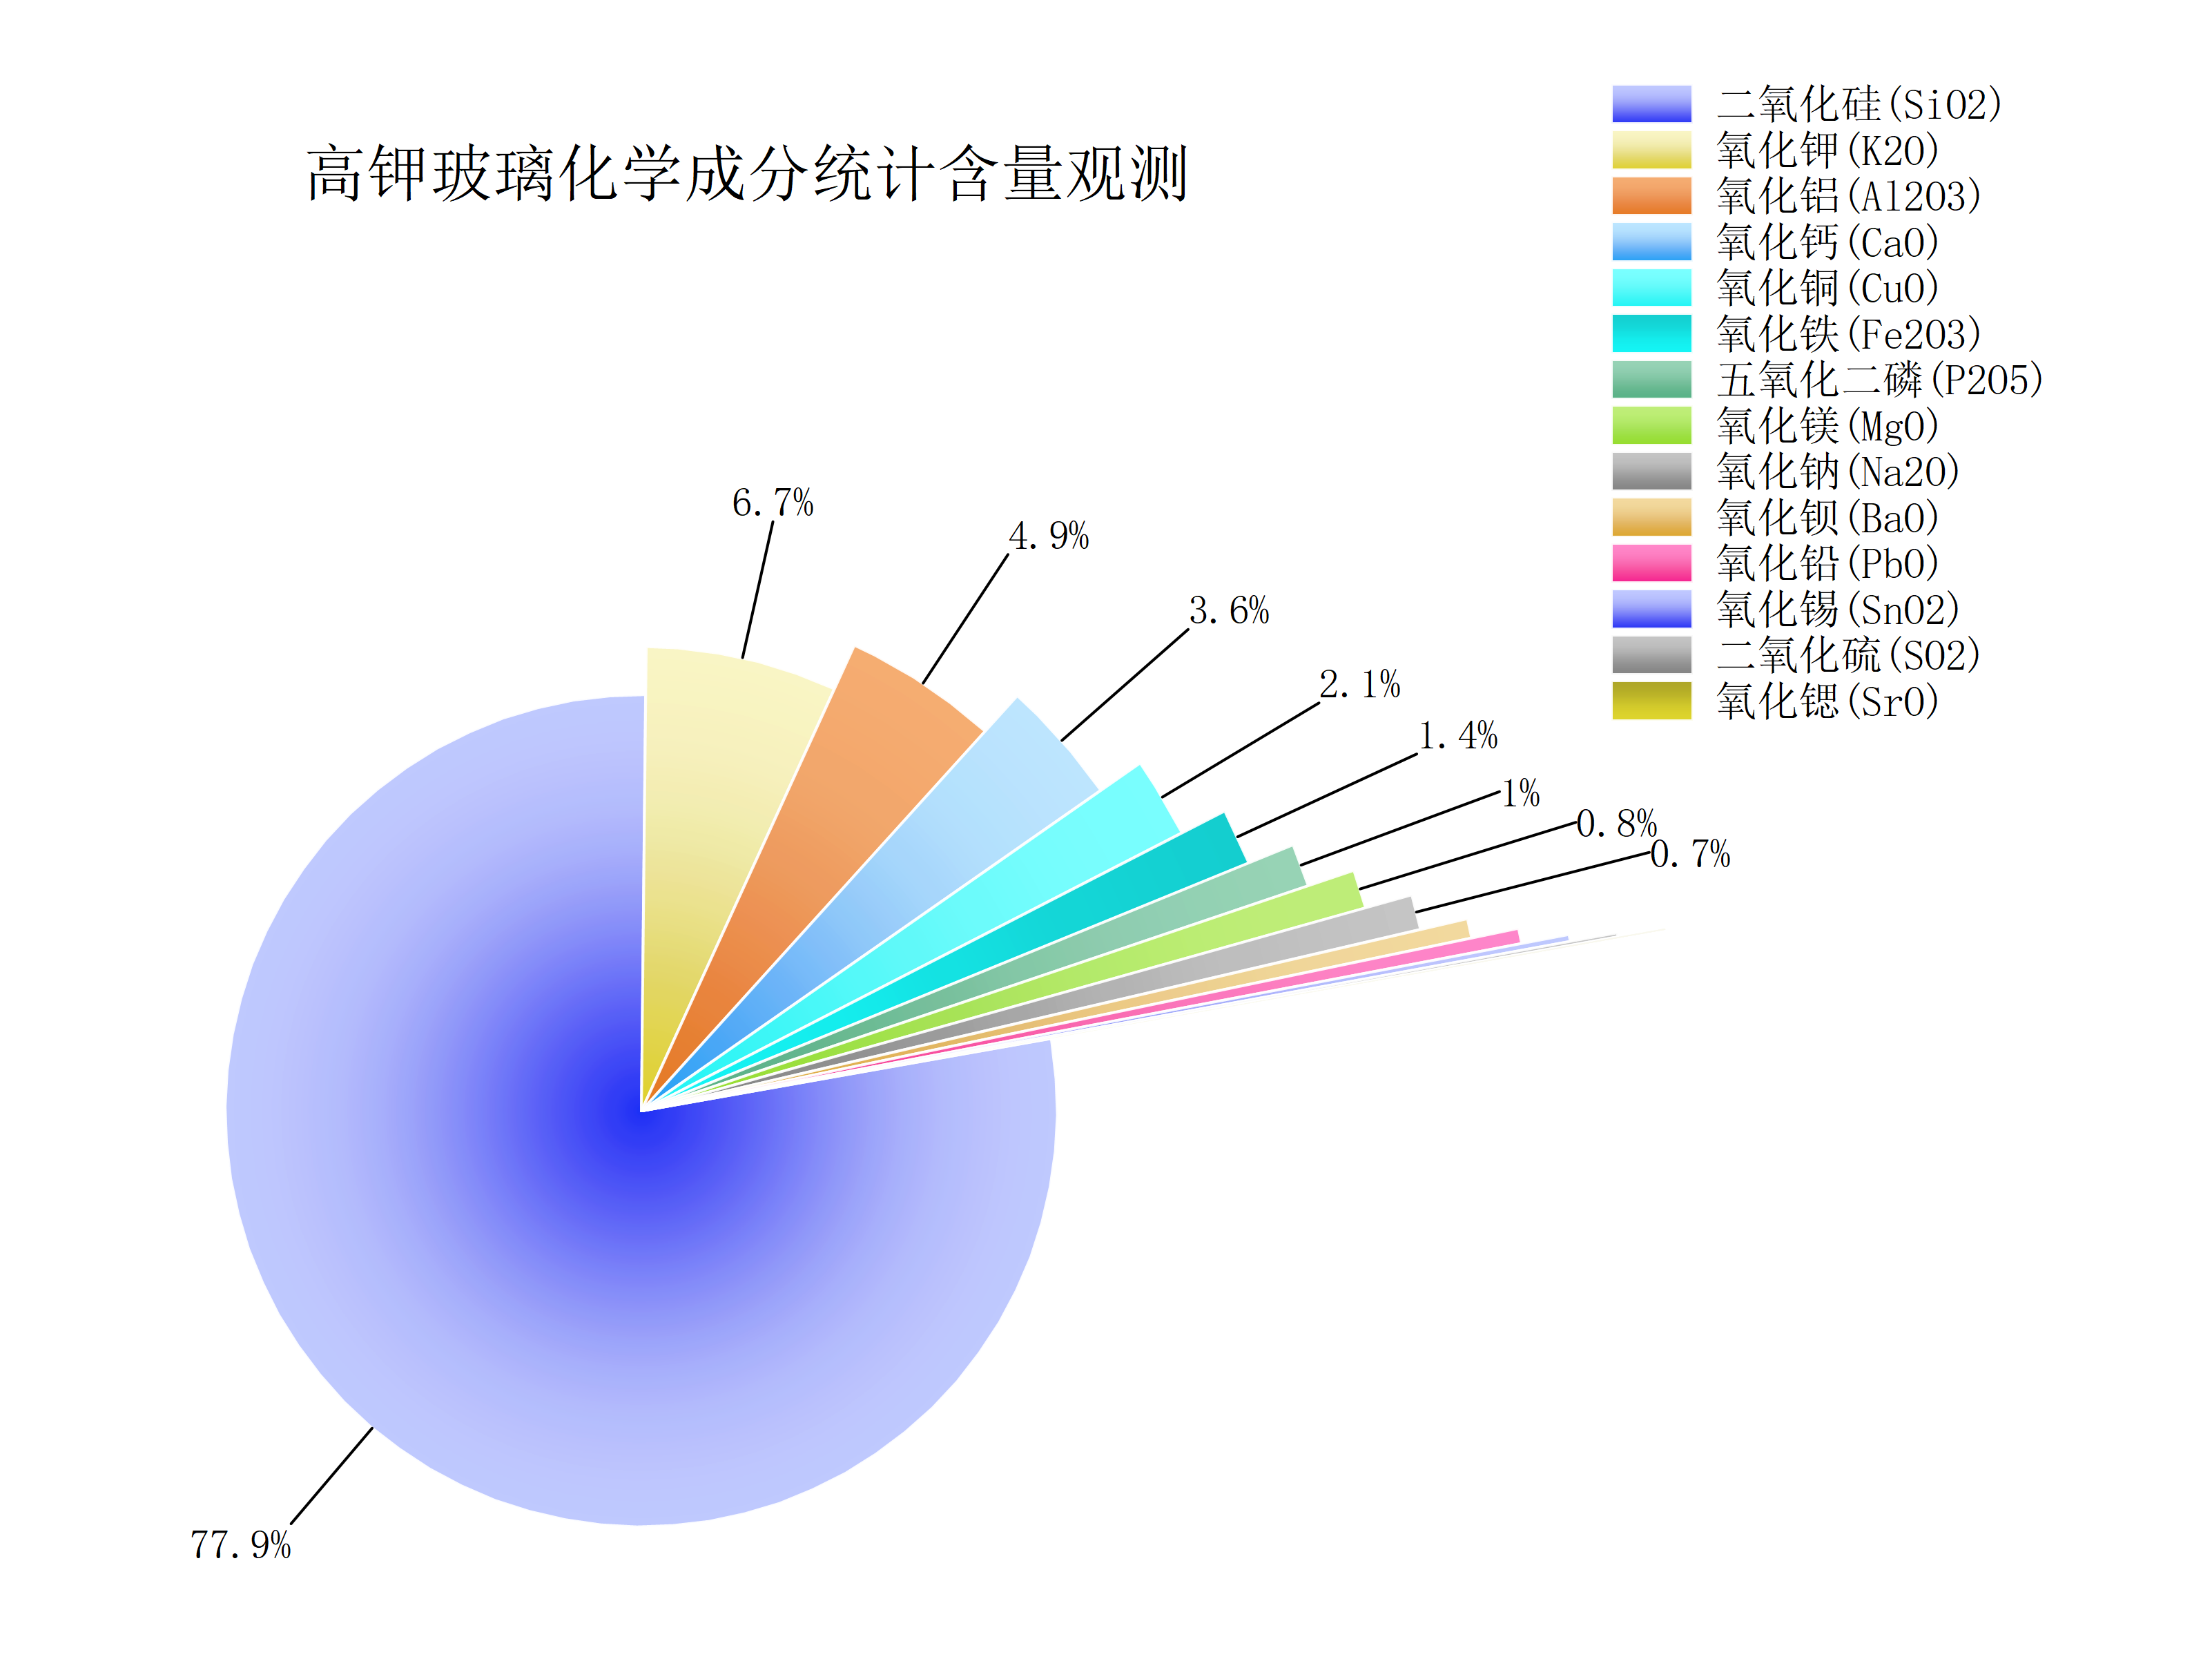
\includegraphics[width=.30\textwidth]{高钾成分侧写}
		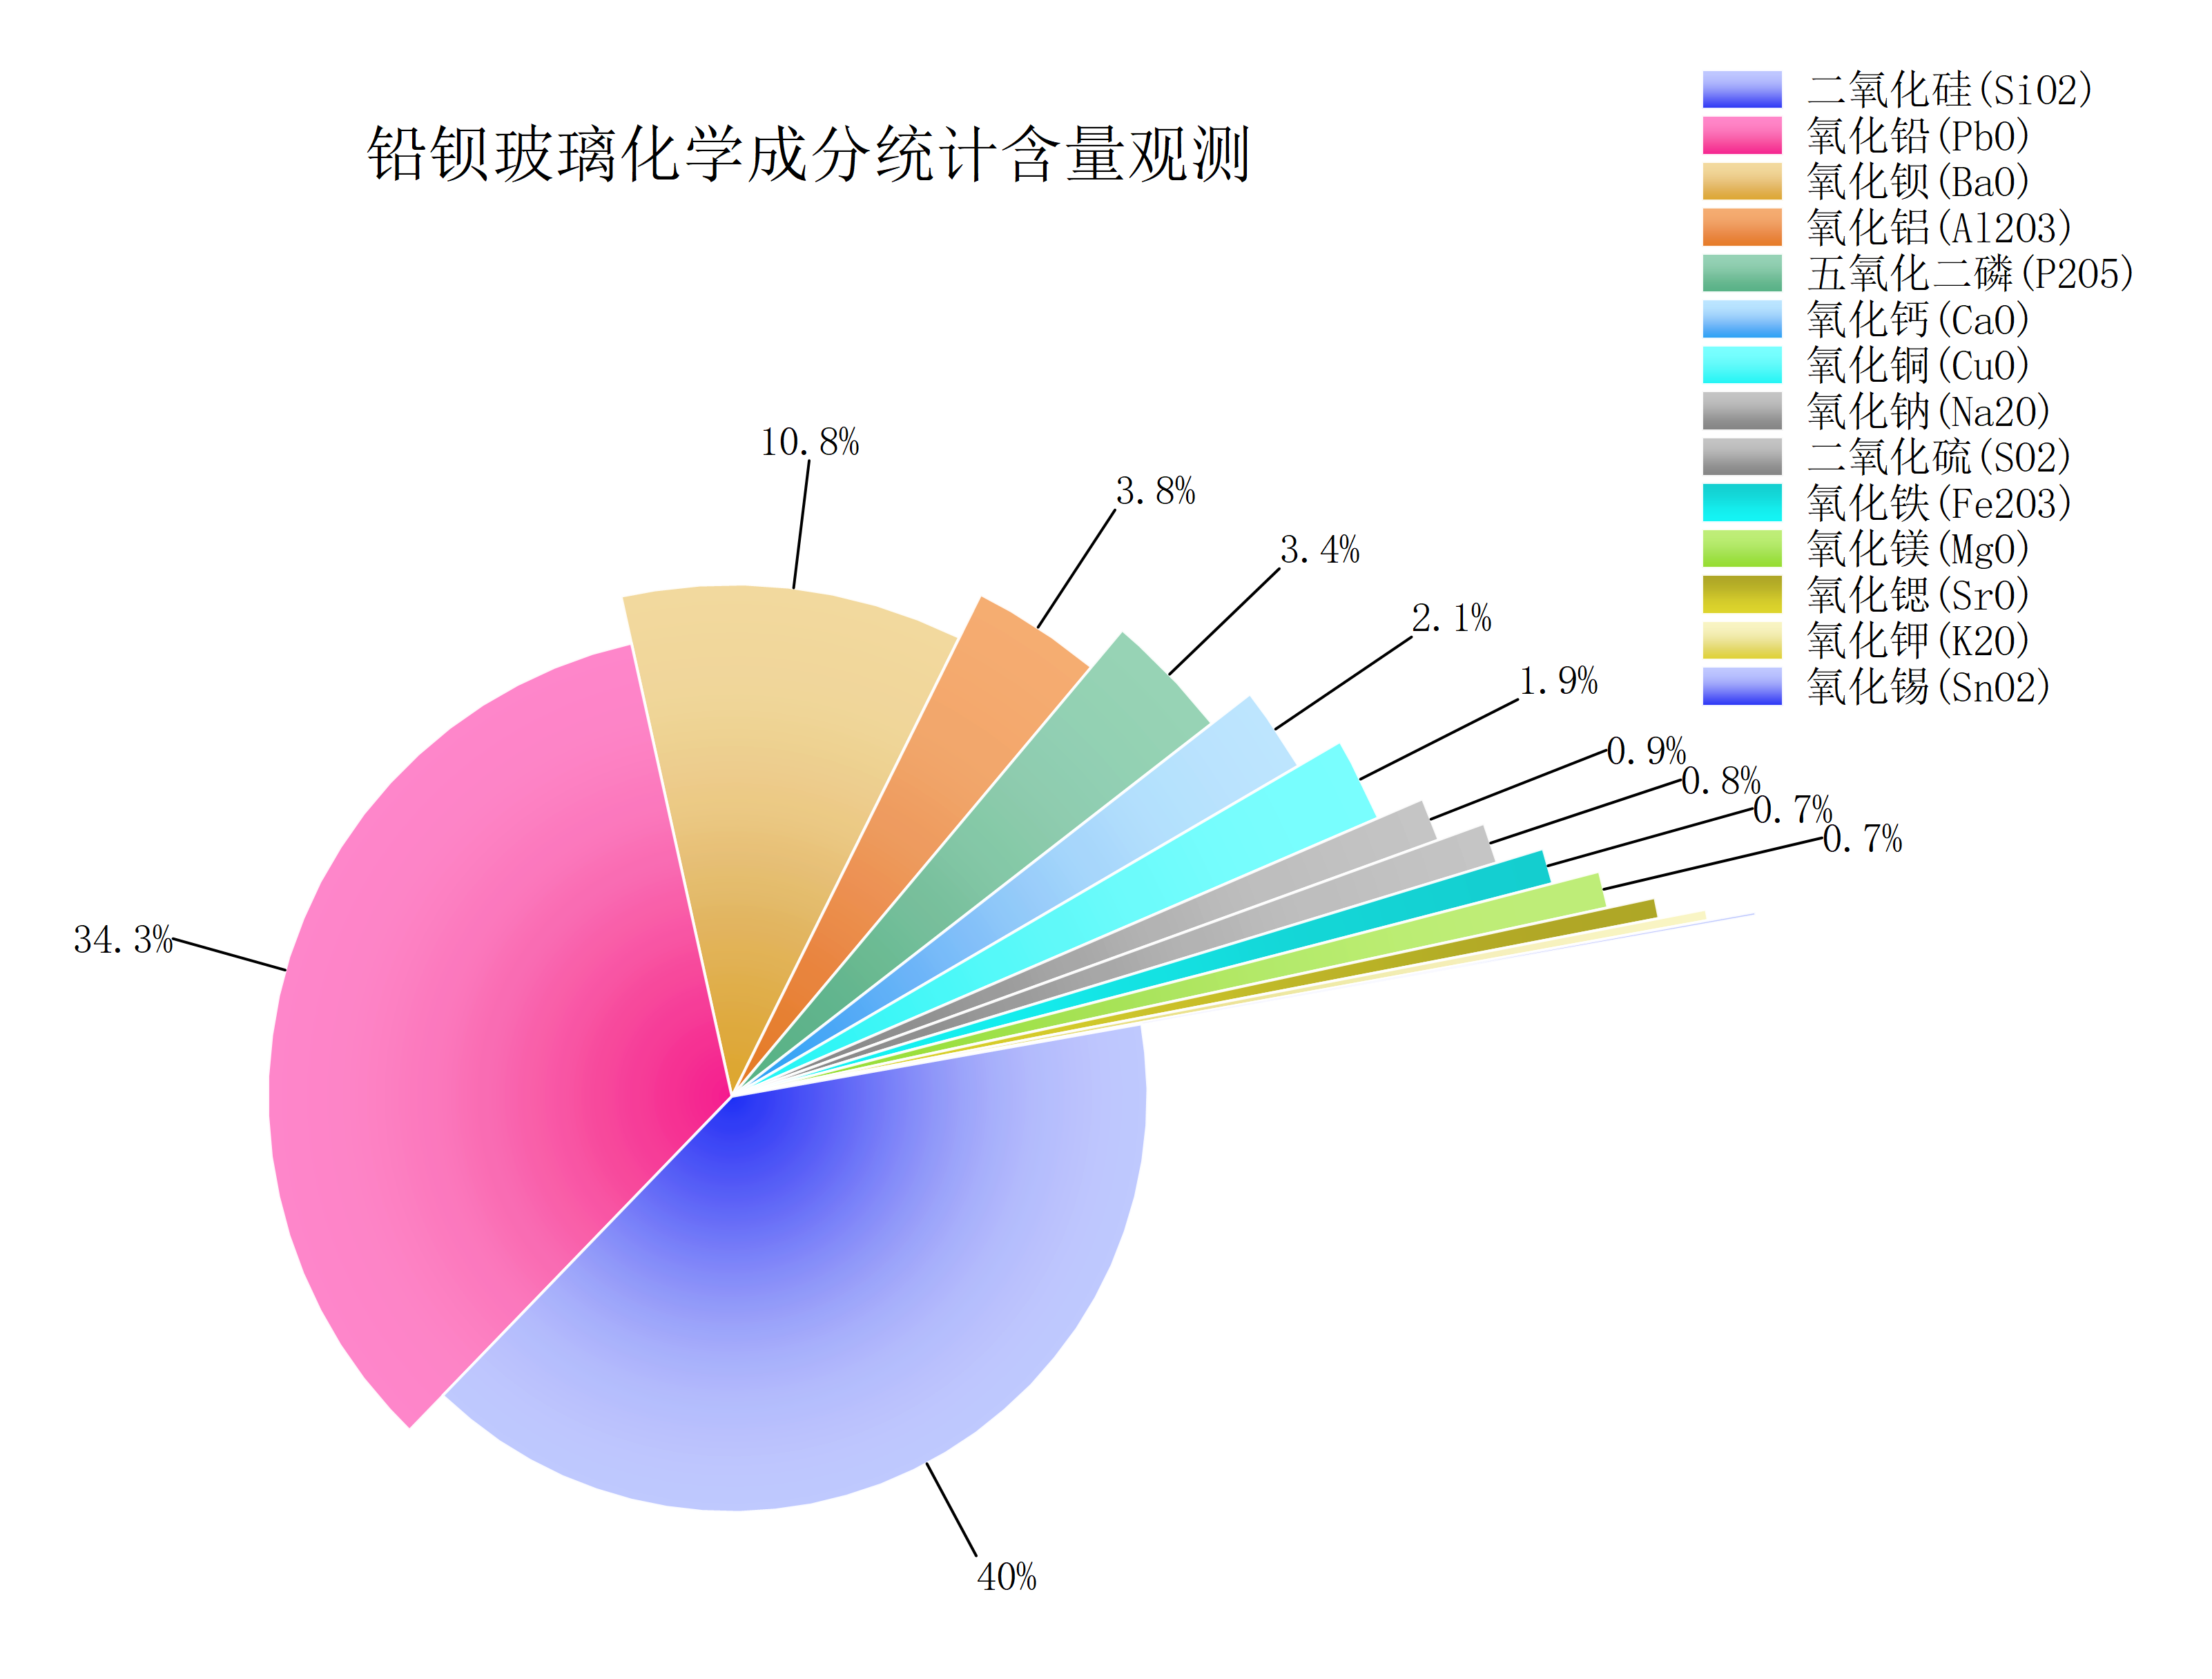
\includegraphics[width=.30\textwidth]{铅钡成分侧写}
		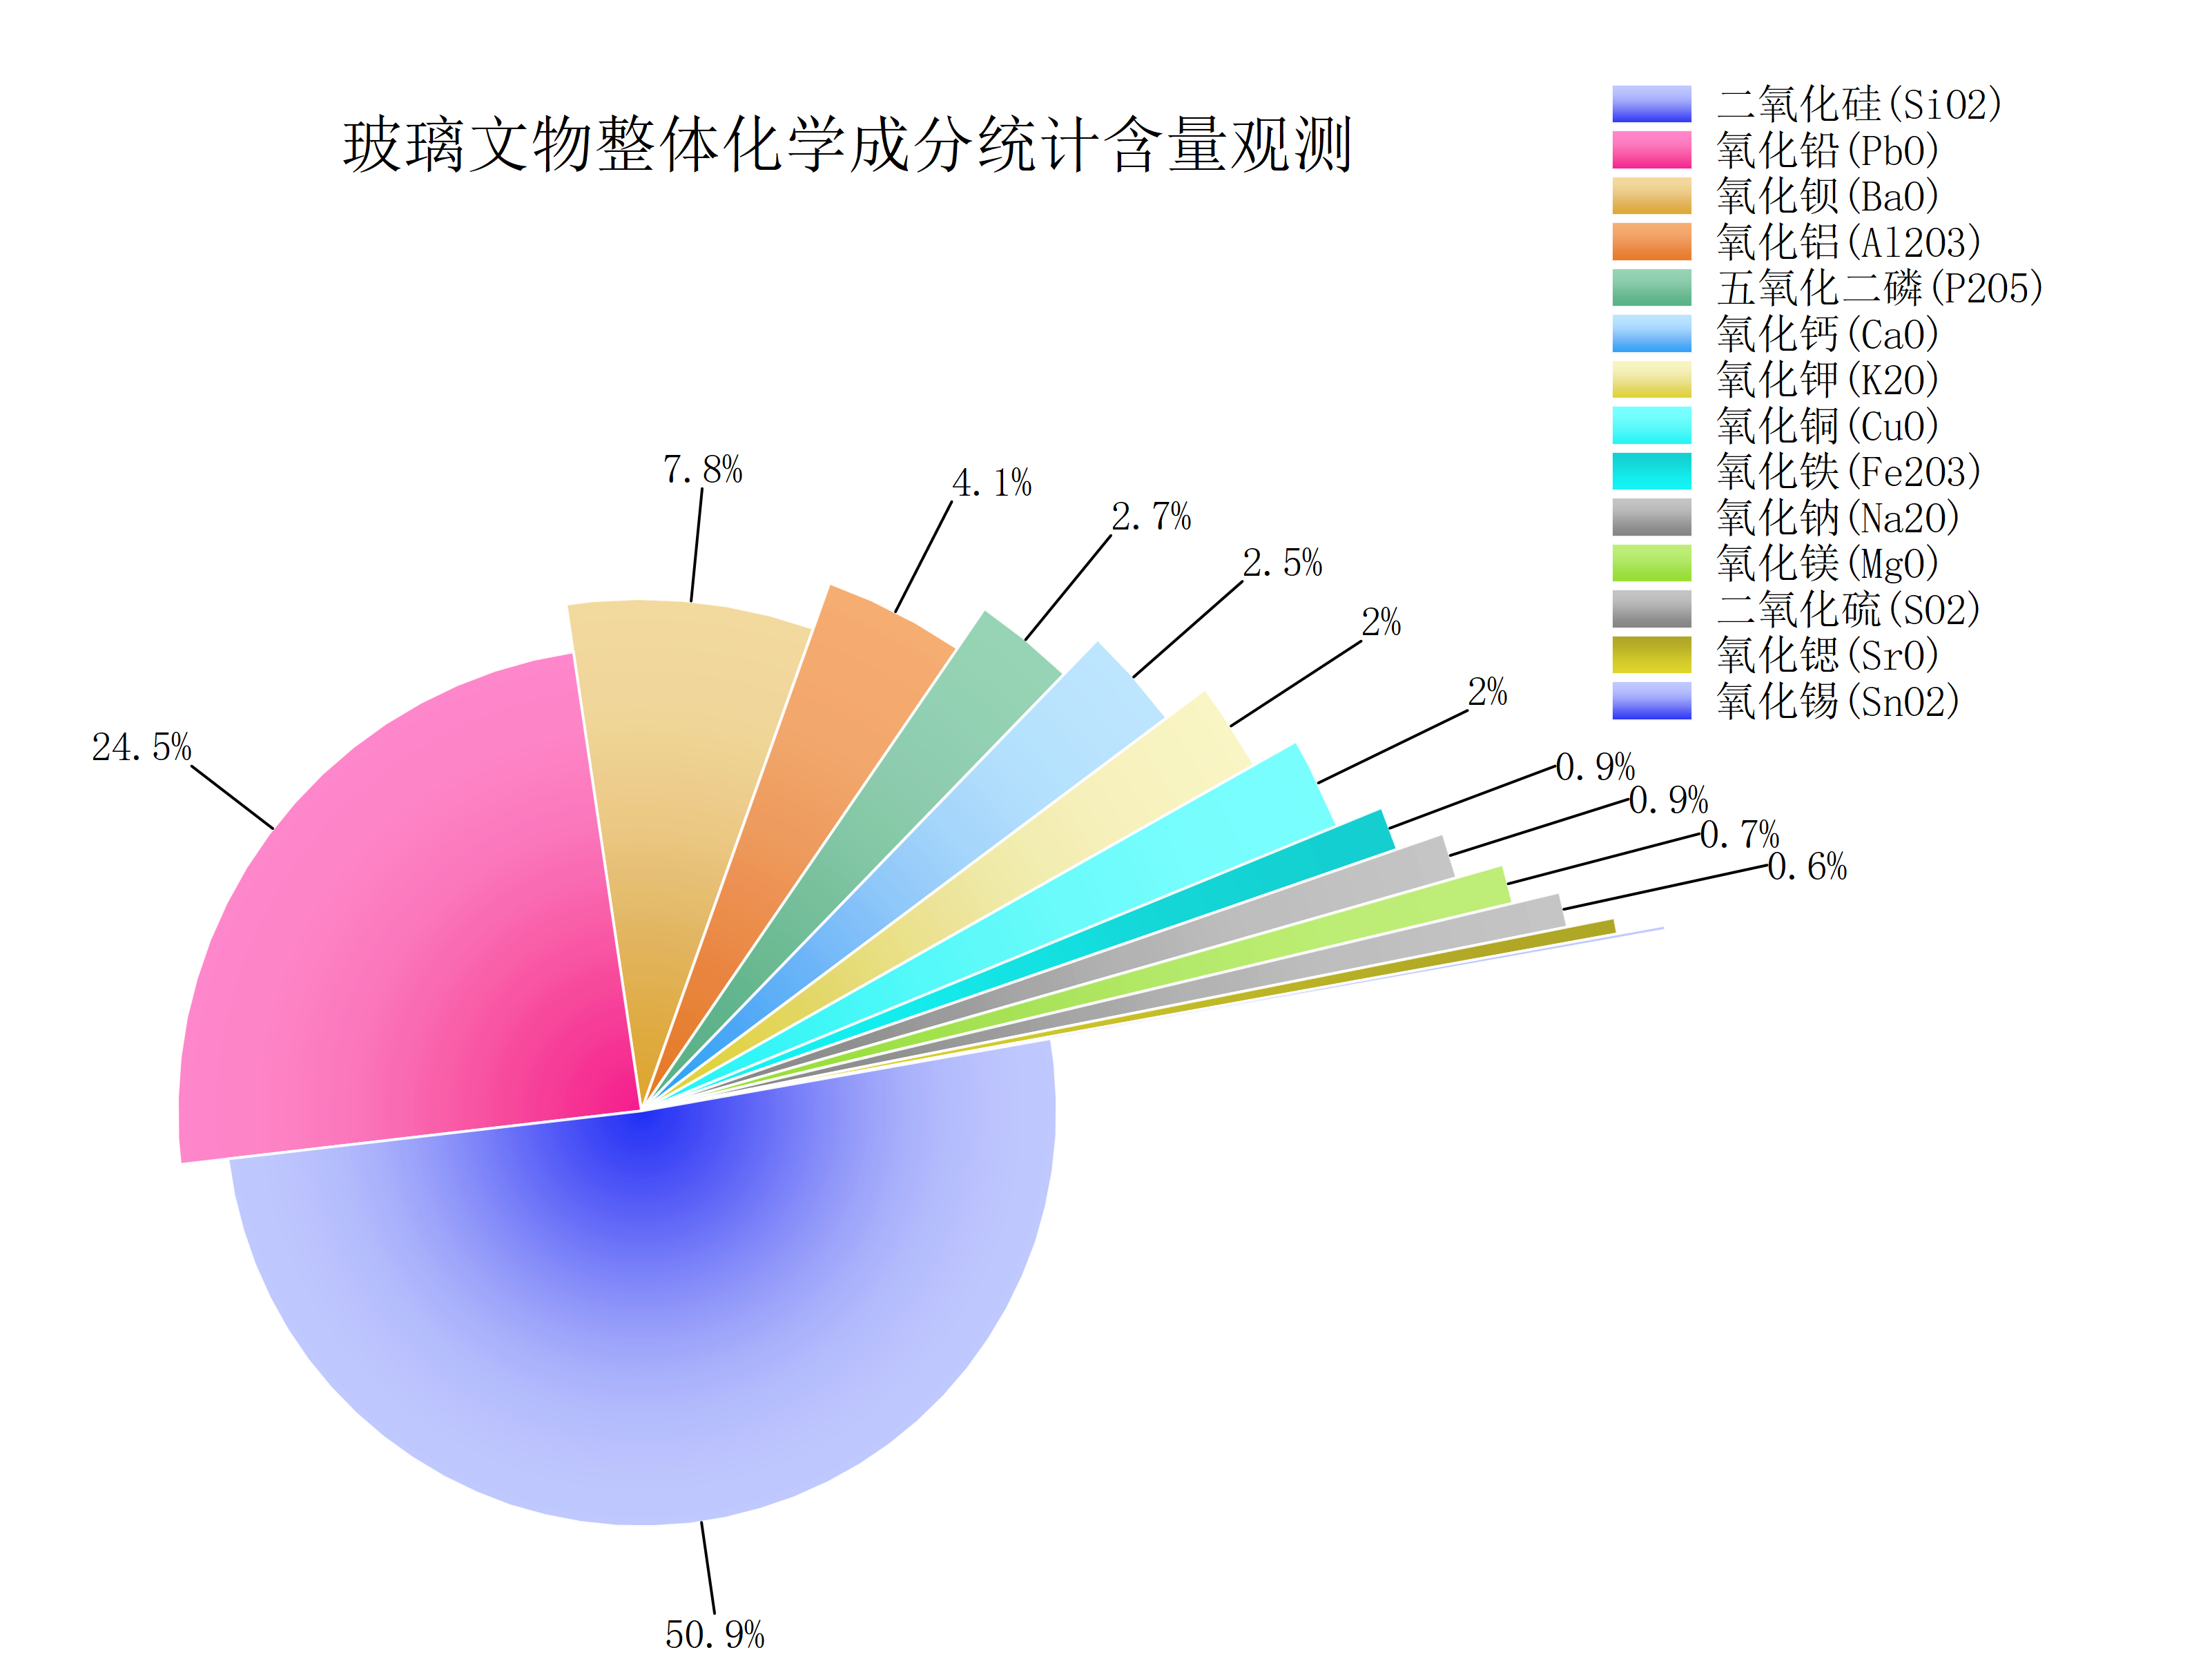
\includegraphics[width=.30\textwidth]{整体成分侧写}
		\caption{化学成分含量组成的数据观测}
		\label{cexie}
	\end{figure}


	由图可得,$SiO_{2}$的化学成分含量最多,高钾玻璃的$K_{2}O$、$CaO$含量较铅钡玻璃类多,铅钡玻璃的$PbO$、$BaO$含量较高钾玻璃类多,符合化学常识,具体问题分析时应该考虑不同成分含量所产生的影响
	
	
	\item 对有无风化的观测 如图\ref{zhuzhuang},为两种玻璃类型的有无表面风化的数据展示。
	
	\begin{figure}[!h]
		\centering
		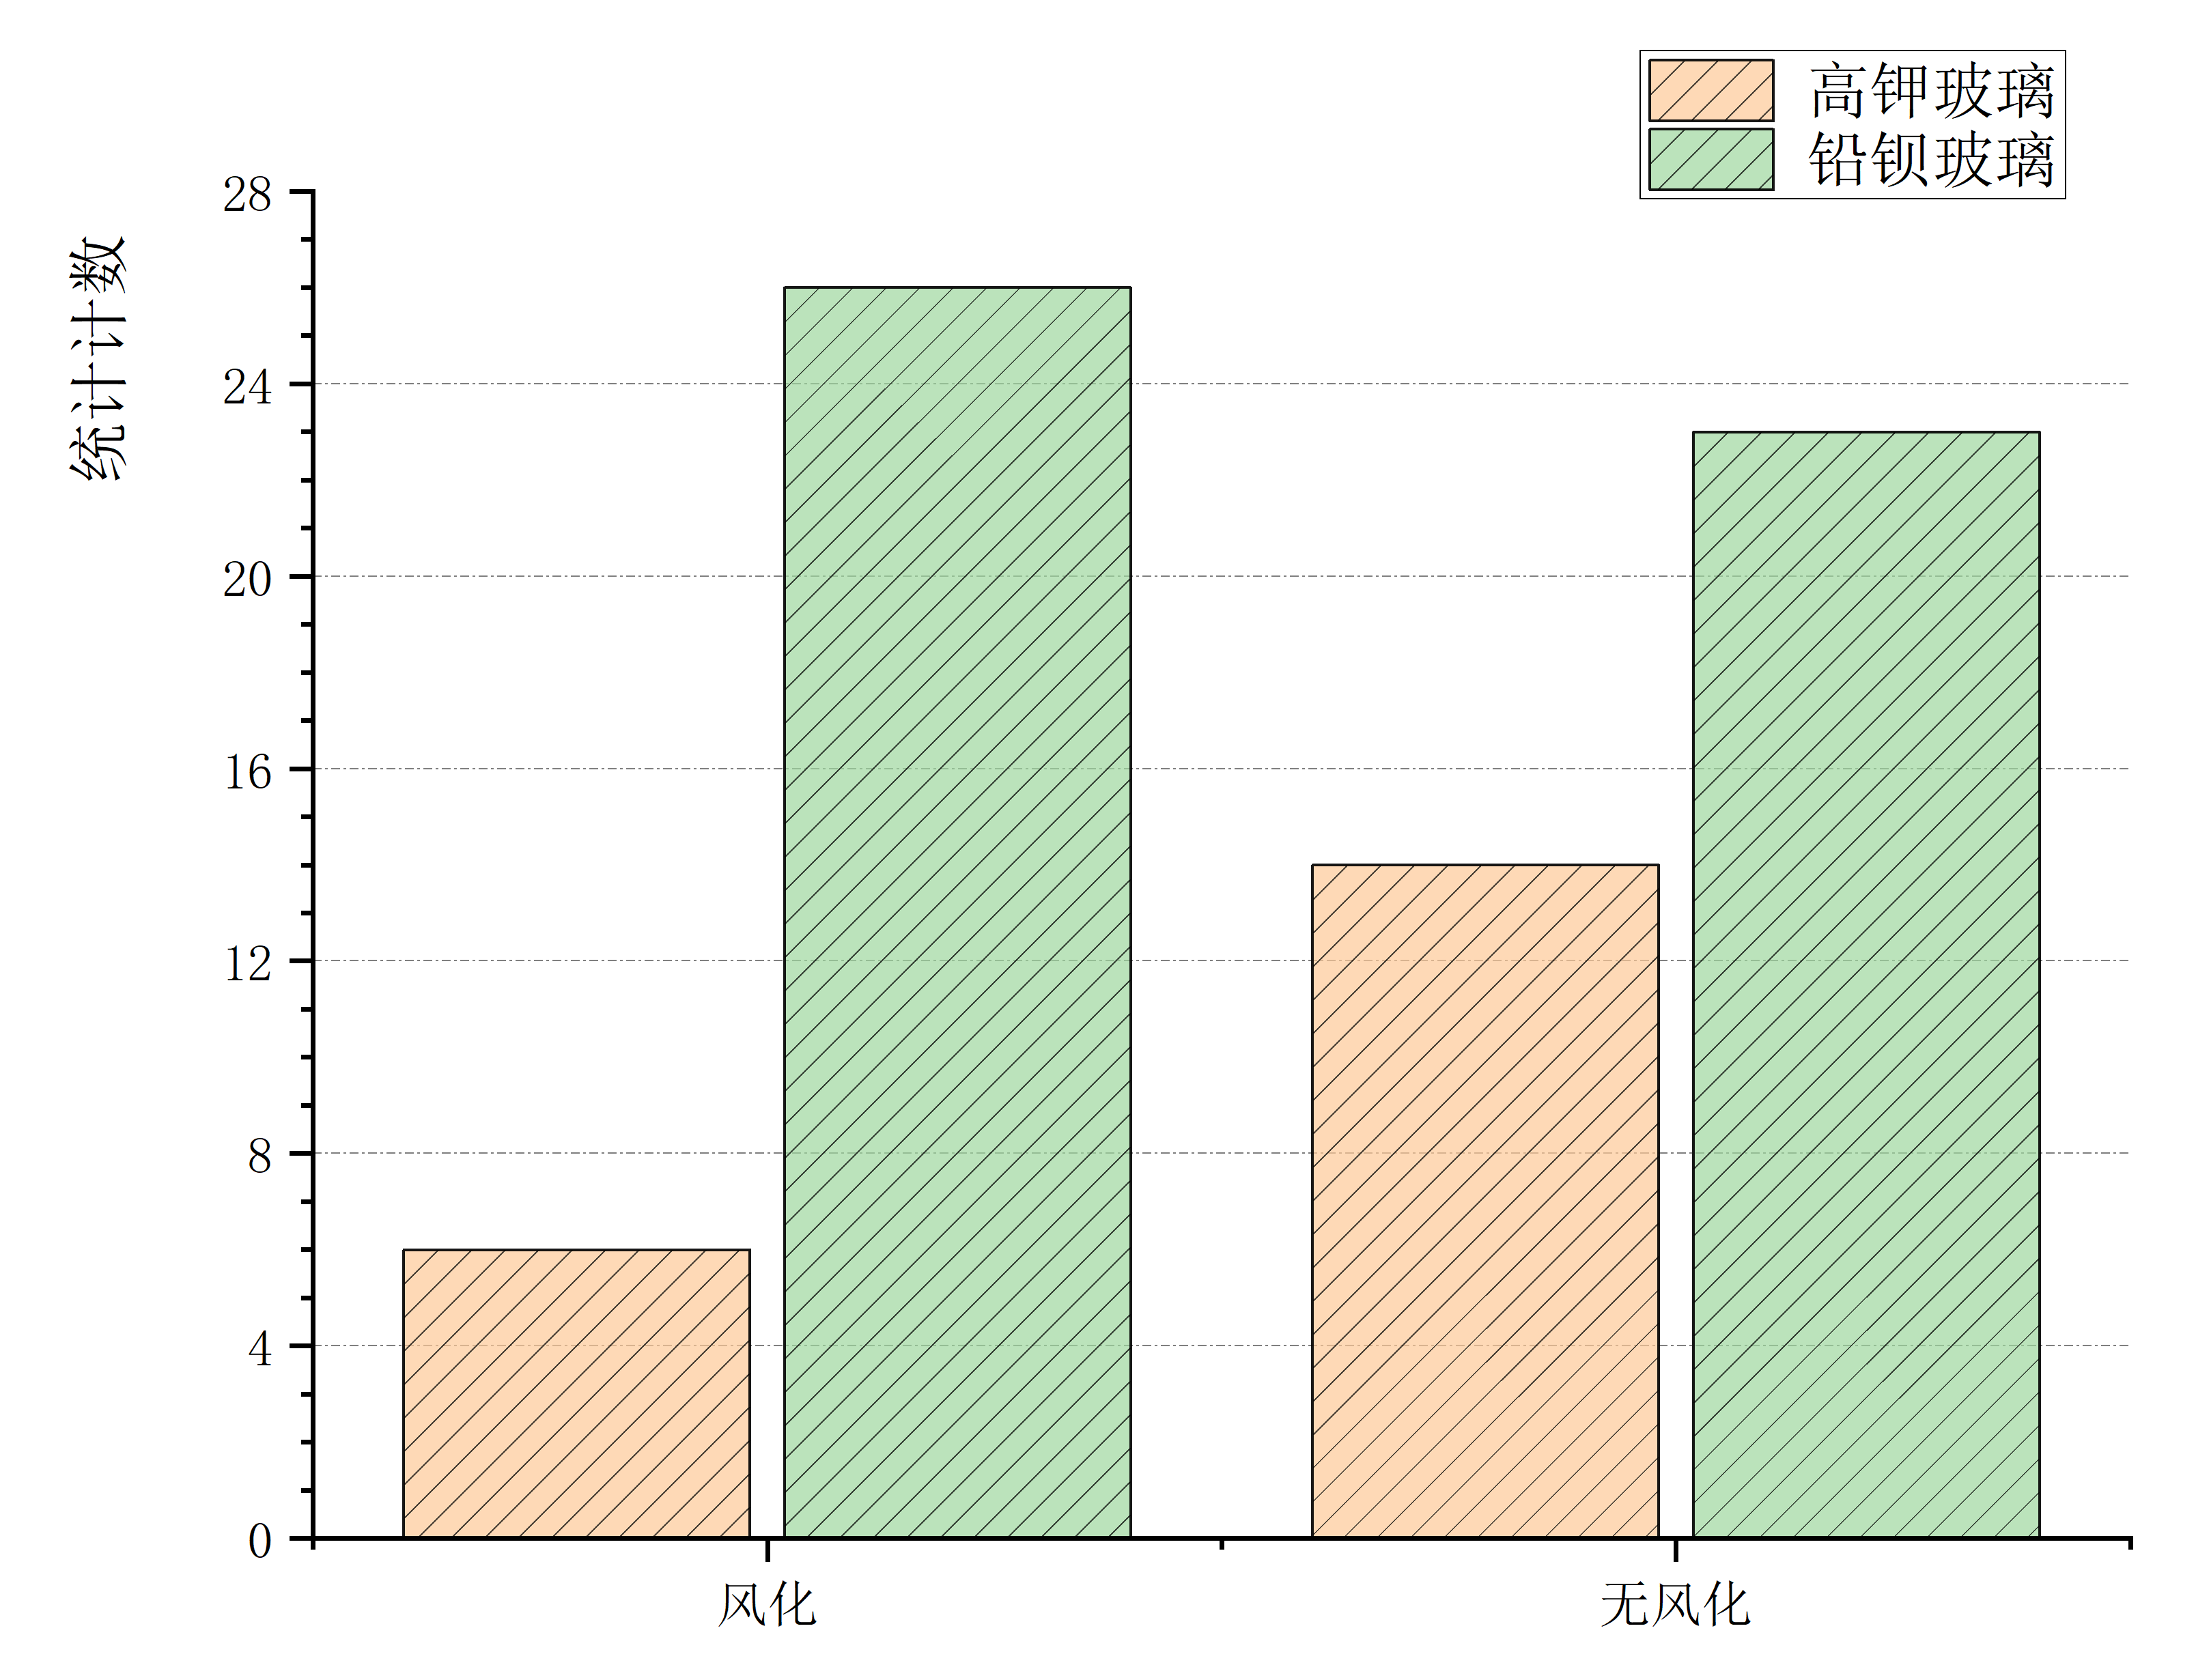
\includegraphics[width=.65\textwidth]{zhuzhuang}
		\caption{两种玻璃类型的有无表面风化的数据观测}
		\label{zhuzhuang}
	\end{figure}
	
	由图可得,铅钡玻璃的风化概率更高,这提示我们风化概率可能与玻璃类型有较大关系。
	
	
\end{itemize}


\section{问题1模型的建立与分析}
\subsection{风化结果与玻璃类型、纹饰与颜色的关系的描述性分析}
首先对数据的整体进行刻画,绘制以玻璃类型、纹饰和颜色为自变量,是否风化为因变量的三维散点气泡图,如图\ref{yuansu3d}所示。

\begin{figure}[!h]
	\centering
	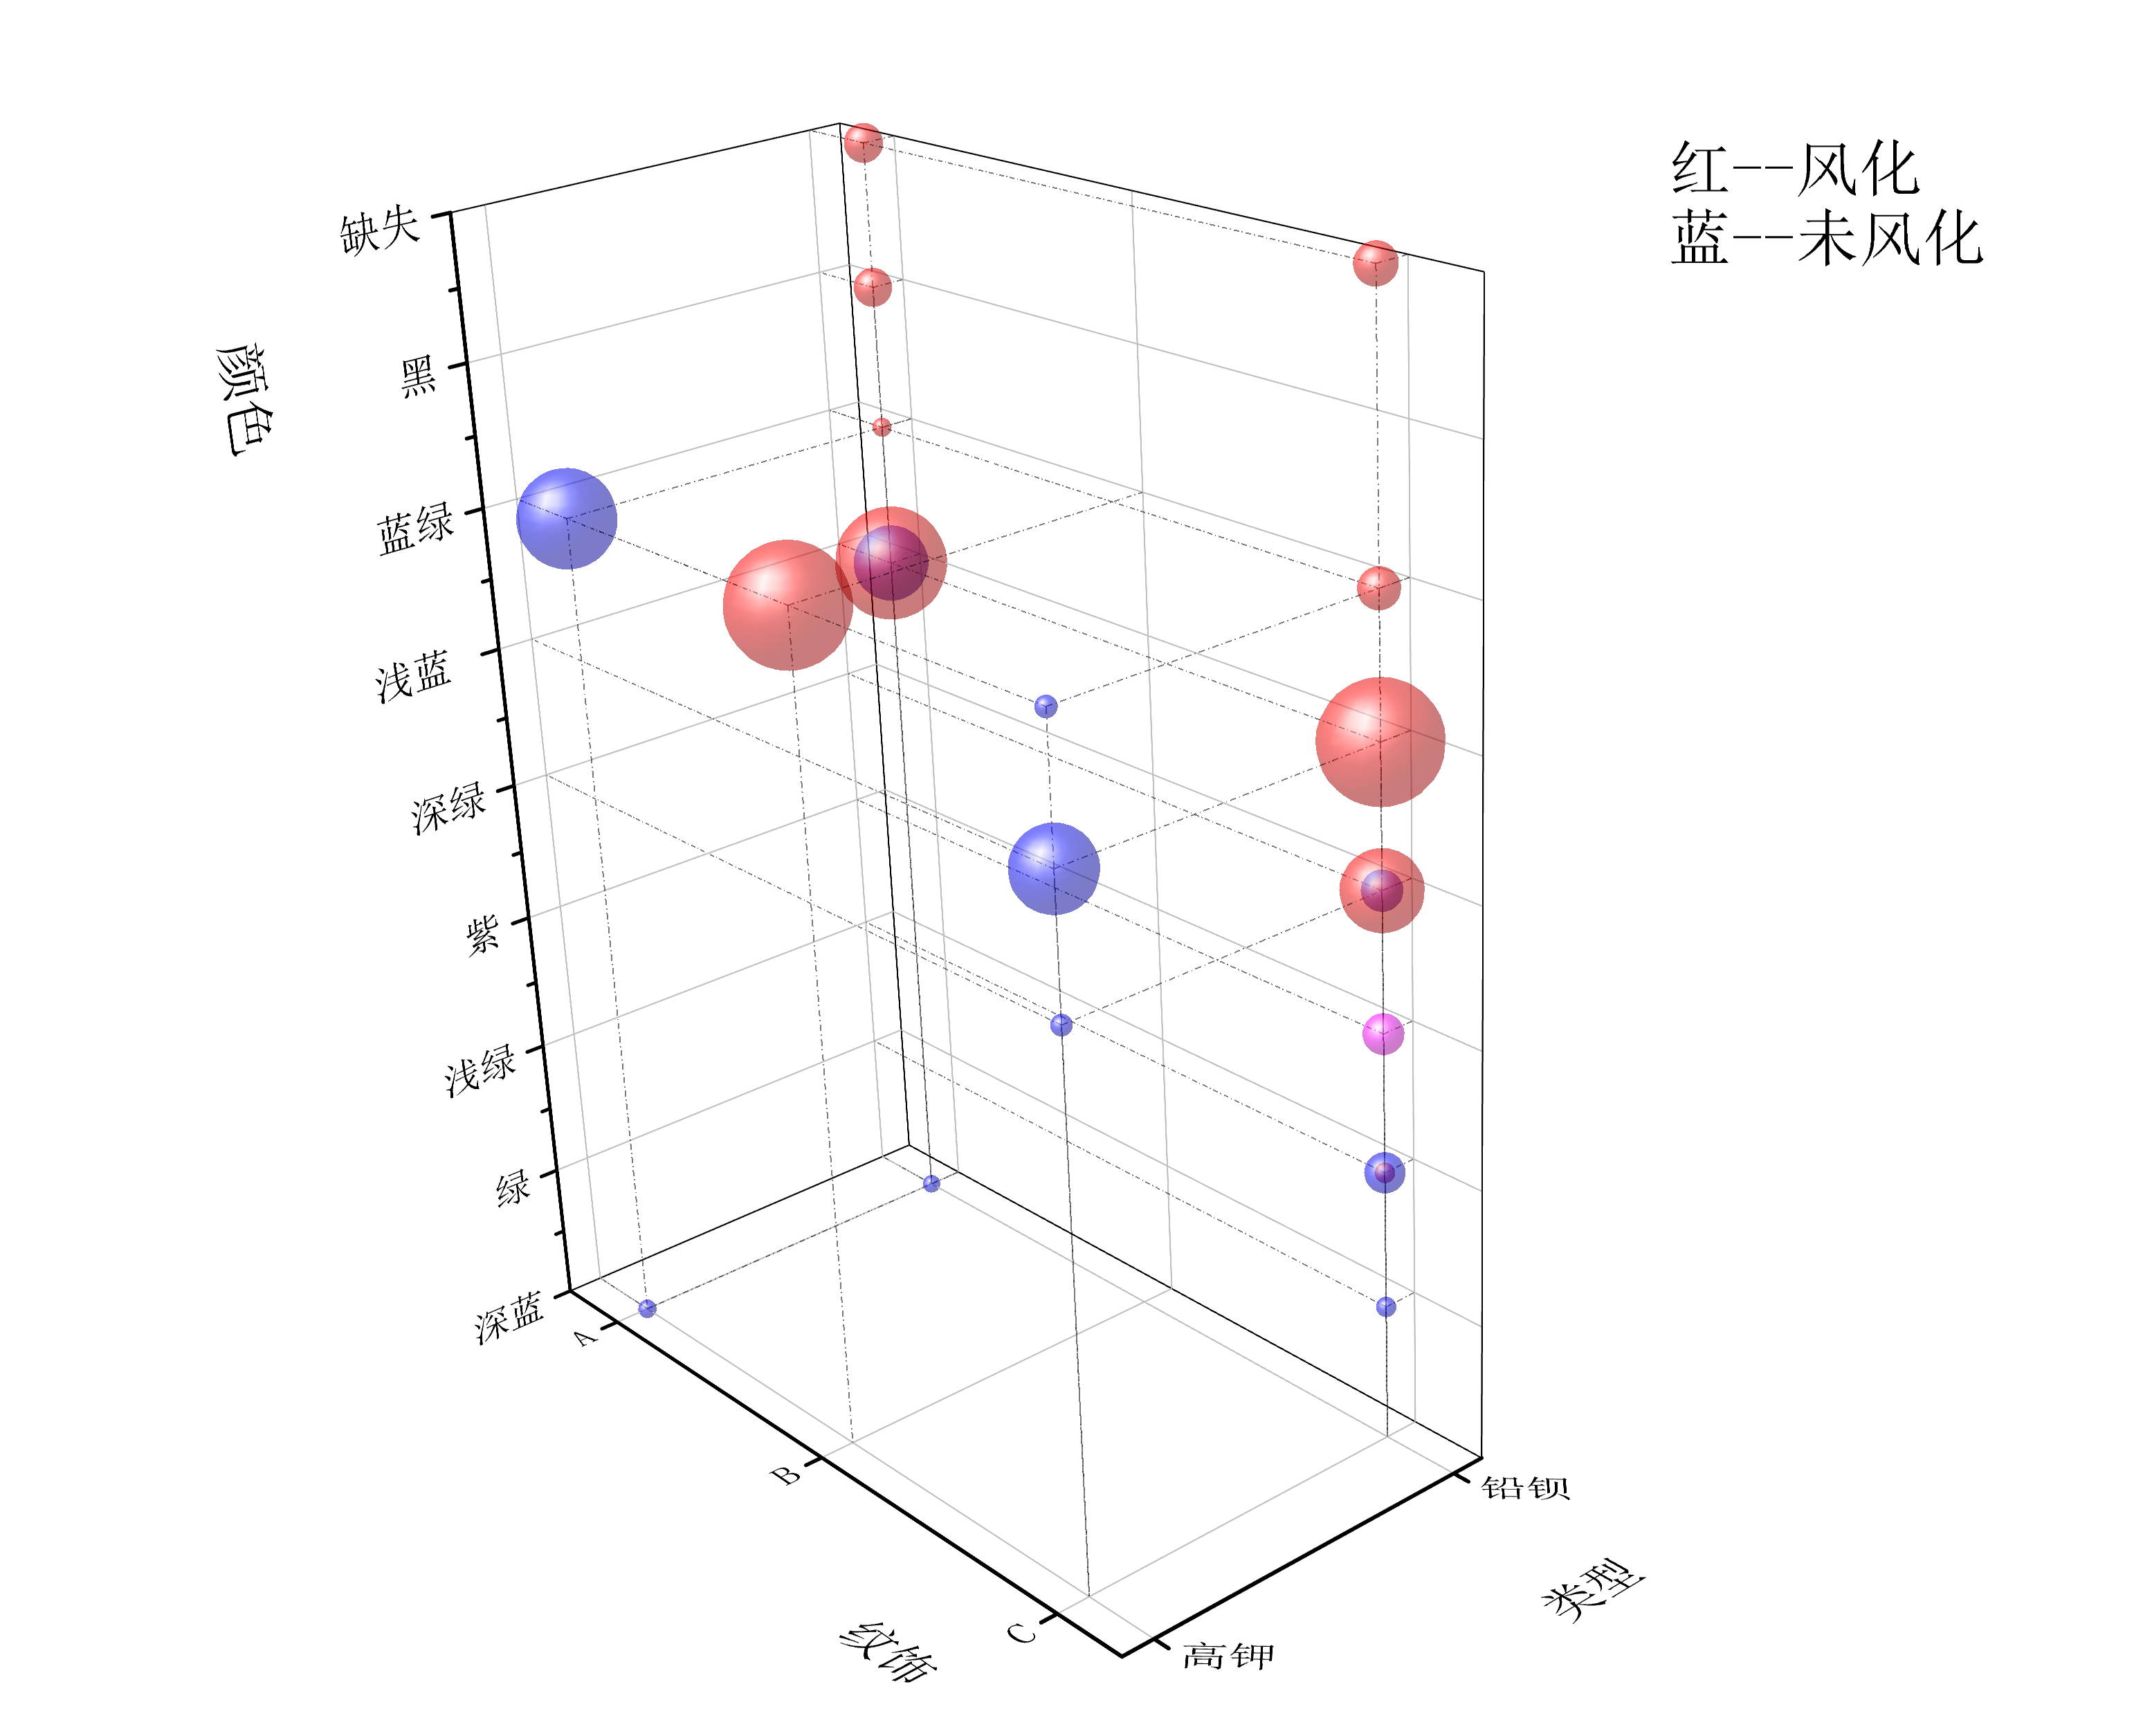
\includegraphics[width=.69\textwidth]{yuansu3d}
	\caption{描述数据整体特征的三维散点气泡图}
	\label{yuansu3d}
\end{figure}


为了得到更加具体的关系特征,对图像进行降维处理,分别得到高钾玻璃和铅钡玻璃的纹饰、颜色与有无分化关系的二维散点图,如图\ref{leixing}所示。

\begin{figure}[!h]
	\centering
	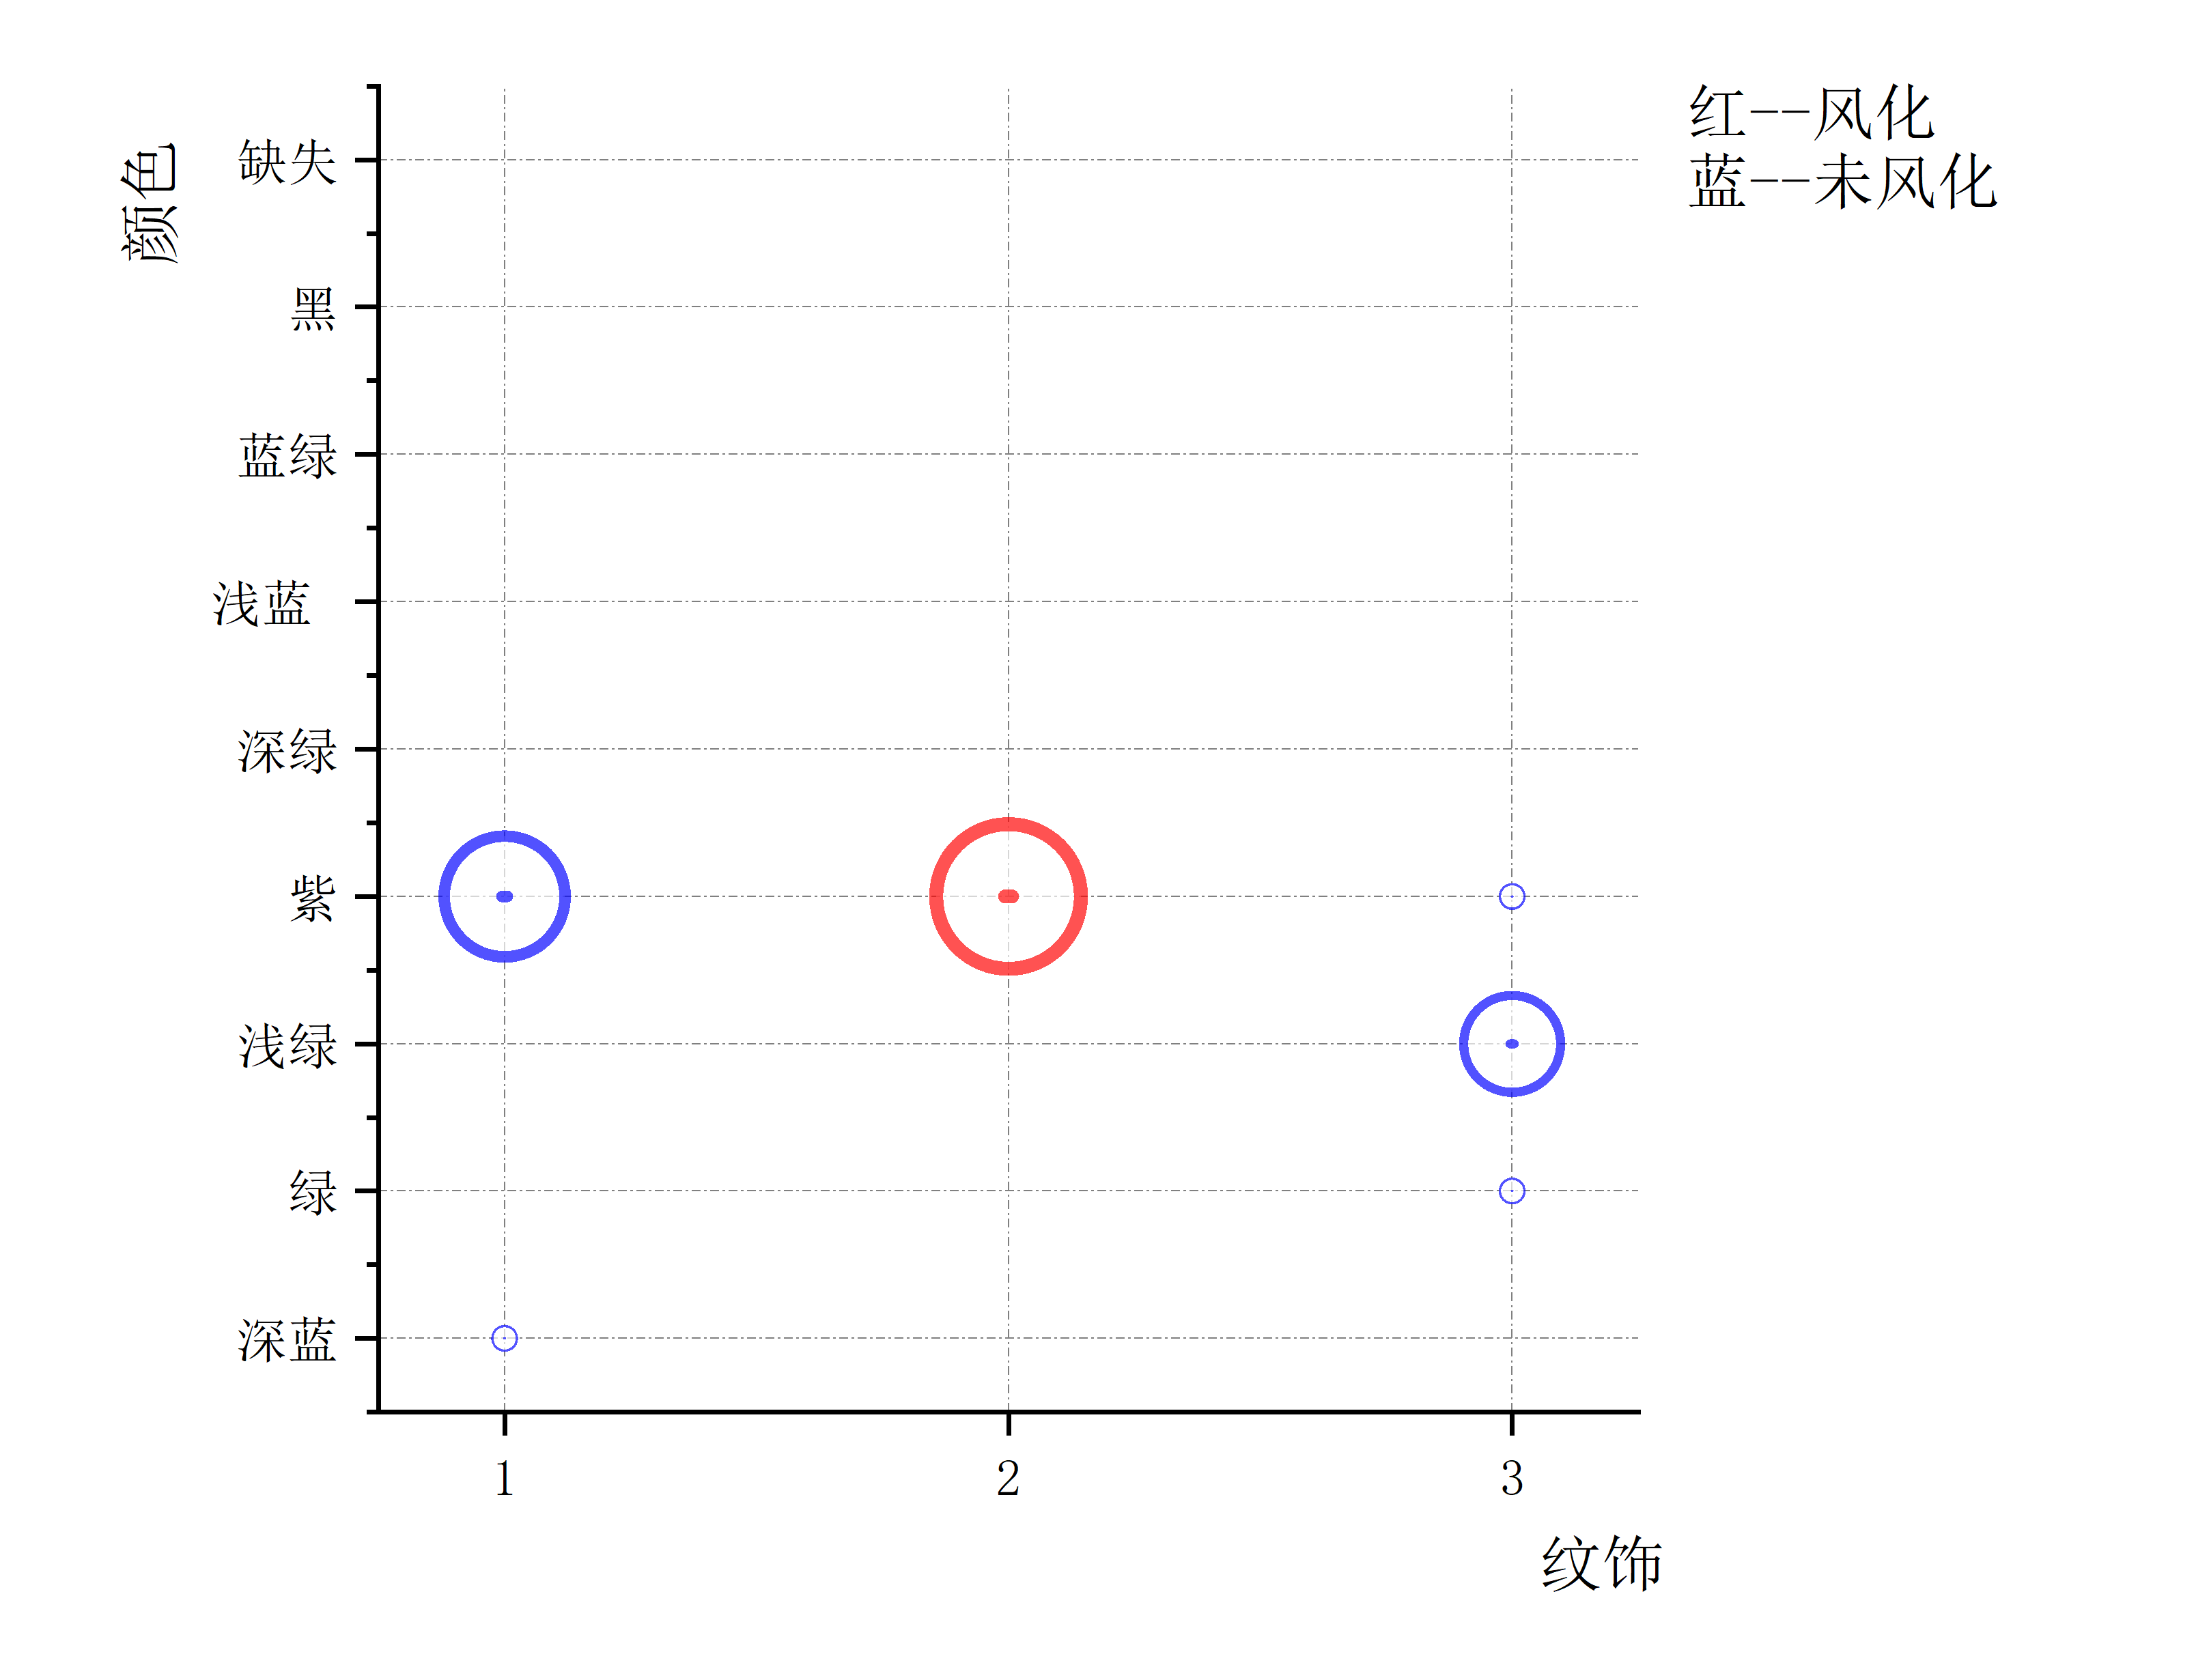
\includegraphics[width=.49\textwidth]{leixing1}
	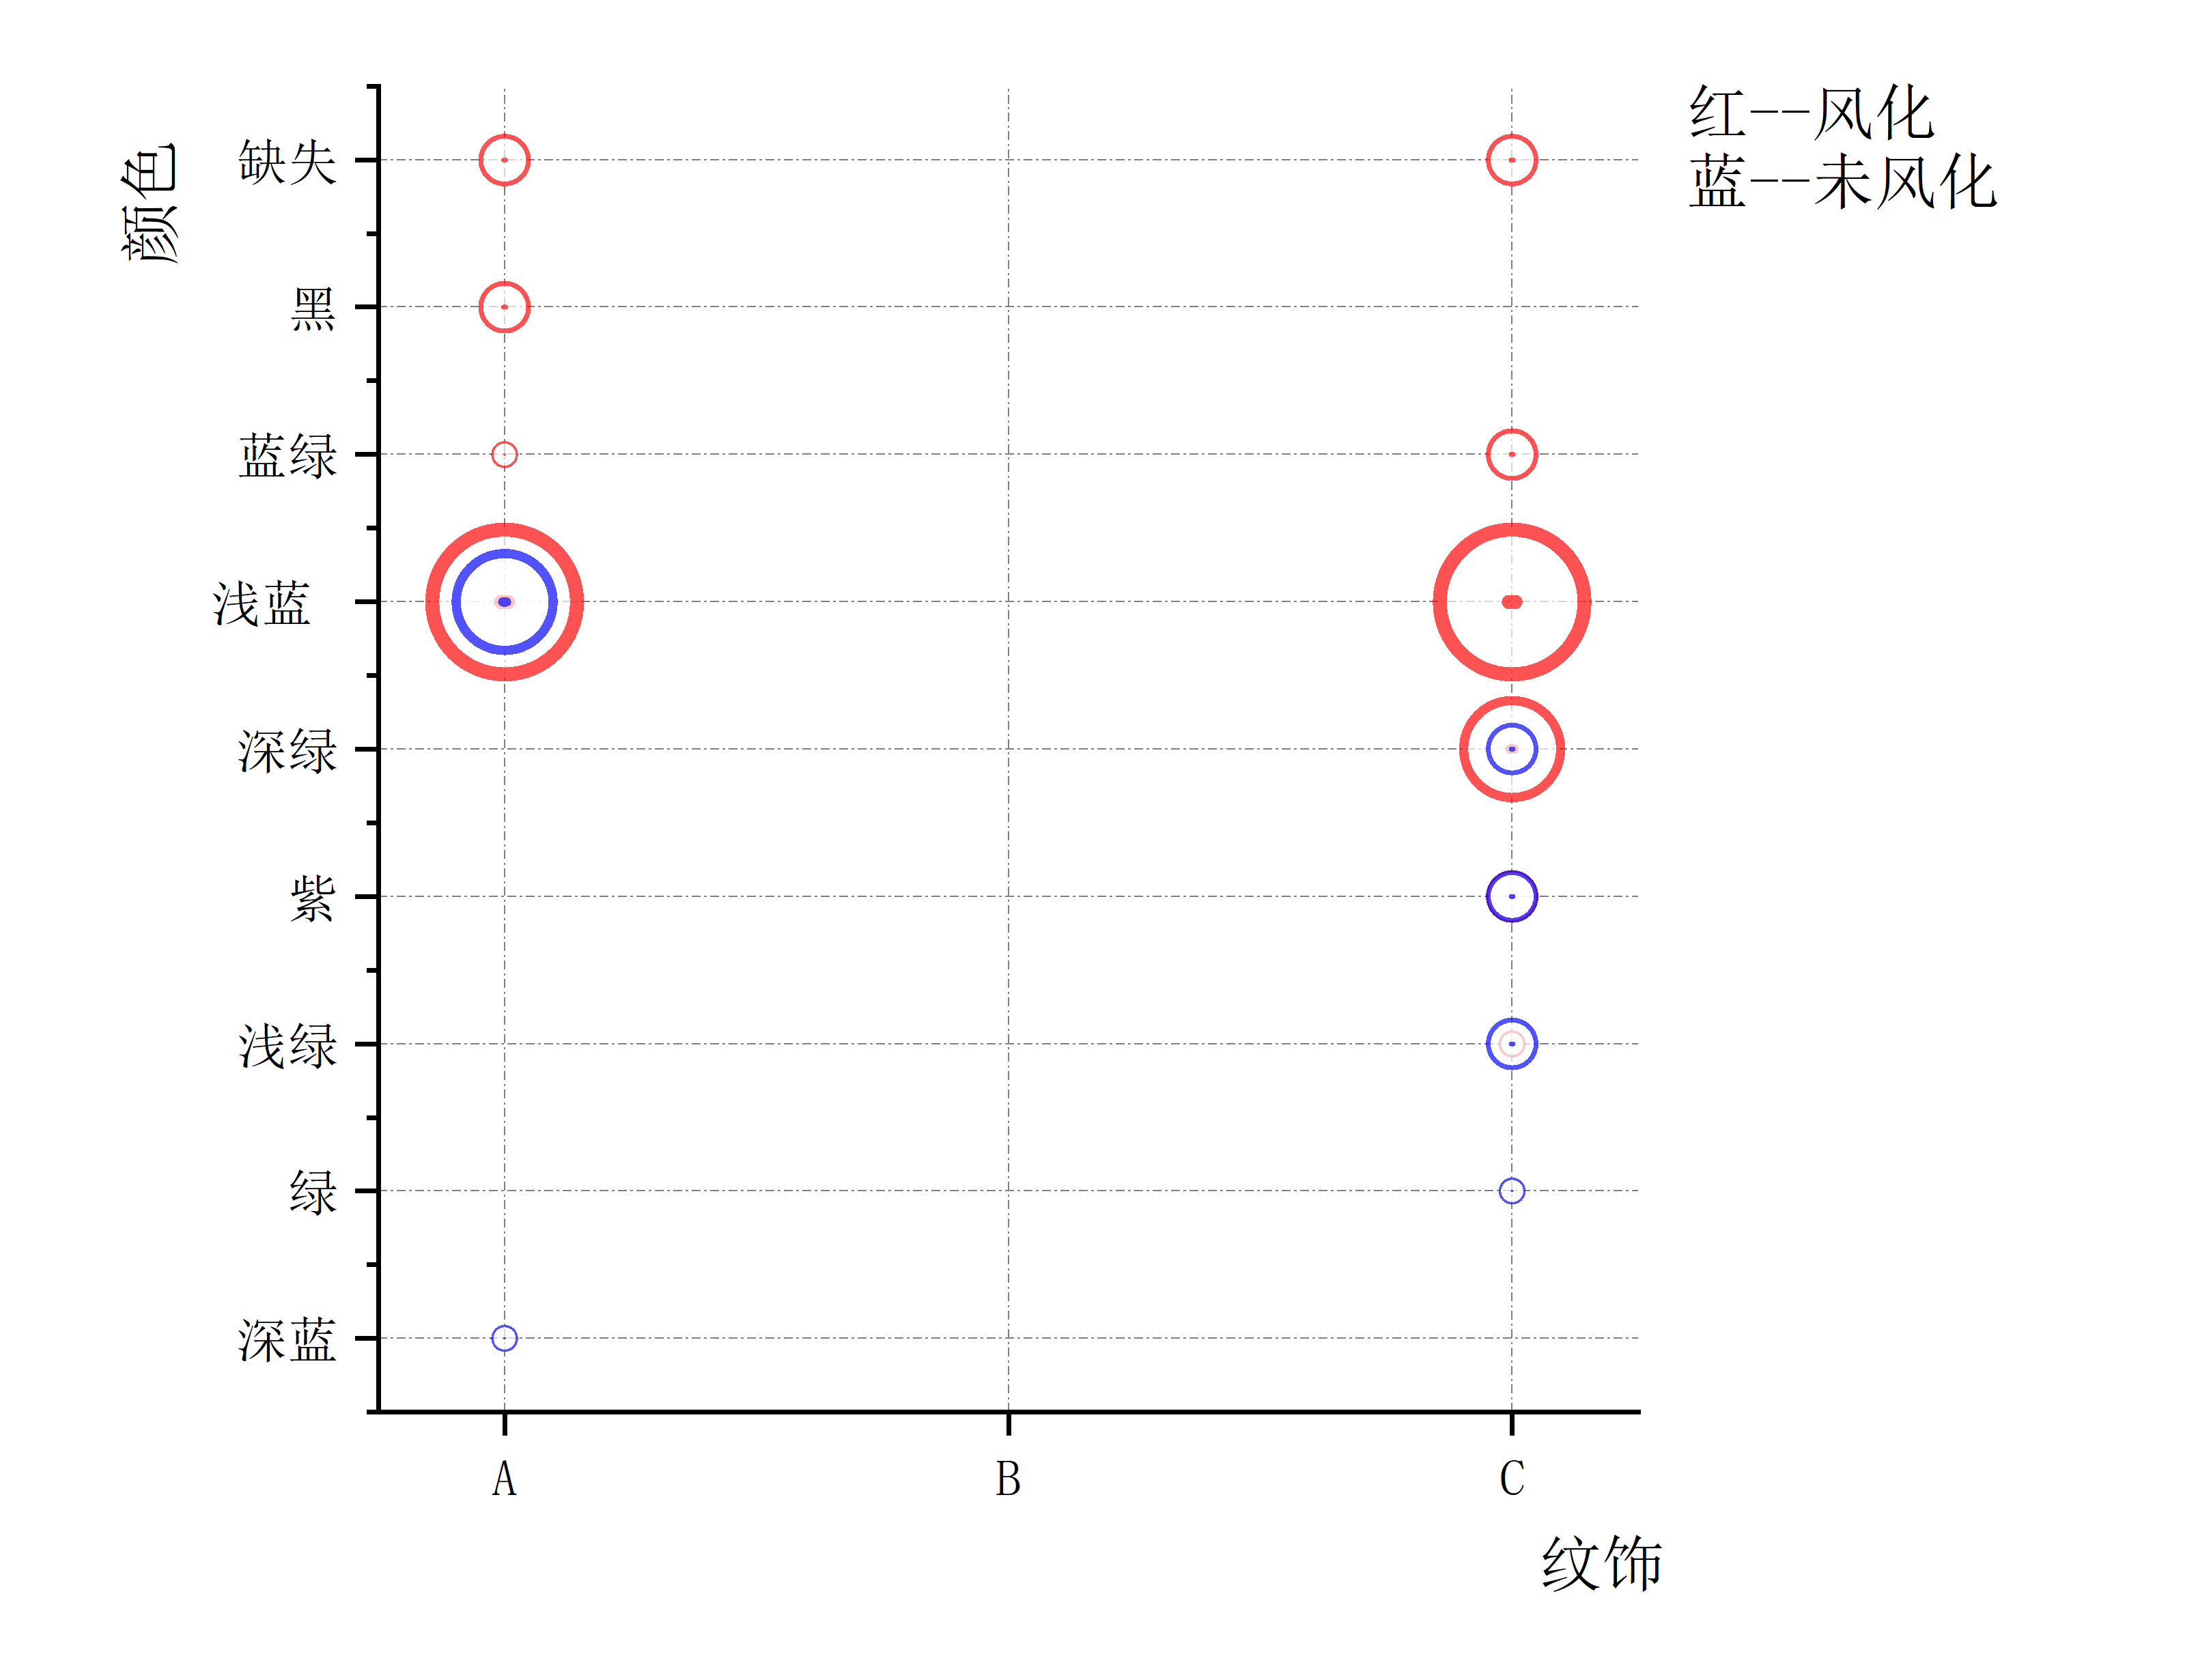
\includegraphics[width=.49\textwidth]{leixing2}
	\caption{描述高钾玻璃(左)和铅钡玻璃(右)数据特征的二维散点图}
	\label{leixing}
\end{figure}


由图,可以得出如下的规律:
\begin{itemize}
	\item 由高钾玻璃的二维图,可以观察到高钾玻璃中B纹饰——紫颜色的种类风化结果表现为风化,且数据样本较多,其他类型的纹饰与颜色均表现为未风化;
	\item 由铅钡玻璃的二维图,可以观察到A纹饰的浅蓝色同时表现出了未风化、风化两种结果,推测当A纹饰的铅钡玻璃介于风化与未风化的过渡地带时,往往呈现出浅蓝色,而A纹饰的其他颜色都具有较好的区分属性,如A纹饰——深蓝色表现为未风化,而A纹饰——蓝绿色/黑色/缺失颜色均表现为风化;
	\item 由铅钡玻璃的二维图,可以观察到C纹饰的深绿色、紫色、浅绿色同时表现出了未风化、风化两种结果,推测当C纹饰的铅钡玻璃介于风化与未风化的过渡地带时,往往呈现出这三种颜色,而C纹饰的其他颜色,如C纹饰——绿色表现为未风化,C纹饰——蓝绿色/缺失颜色均表现为风化。
\end{itemize}


基于上述的规律,本文做出了三个维度数据与风化结果的关系特征的推导:
\begin{itemize}
	\item 玻璃类型会对风化结果产生较显著的影响,铅钡玻璃风化比重比高钾玻璃大
	\item 风化过程中会存在颜色的渐变,这种渐变过程会因玻璃类型和纹饰存在差异,如铅钡玻璃的C纹饰,初始为绿色,经过风化由于化学成分改变逐渐变成浅绿、深绿的过度颜色,最终被完全风化,变成蓝绿色。
\end{itemize}


\subsection{基于Spearman相关系数的按含量比例分类的分类模型}

本文设计了基于Spearman相关系数的按含量比例分类的模型,具体流程如下所示:

首先针对高钾玻璃做具体的流程分析:
\begin{itemize}
	\item Step1: 绘制高钾玻璃风化前后的各个归一化后的化学成分含量的散点图如图\ref{gjfh}(左)所示,观察数据特征。
	
	\begin{figure}[!h]
		\centering
		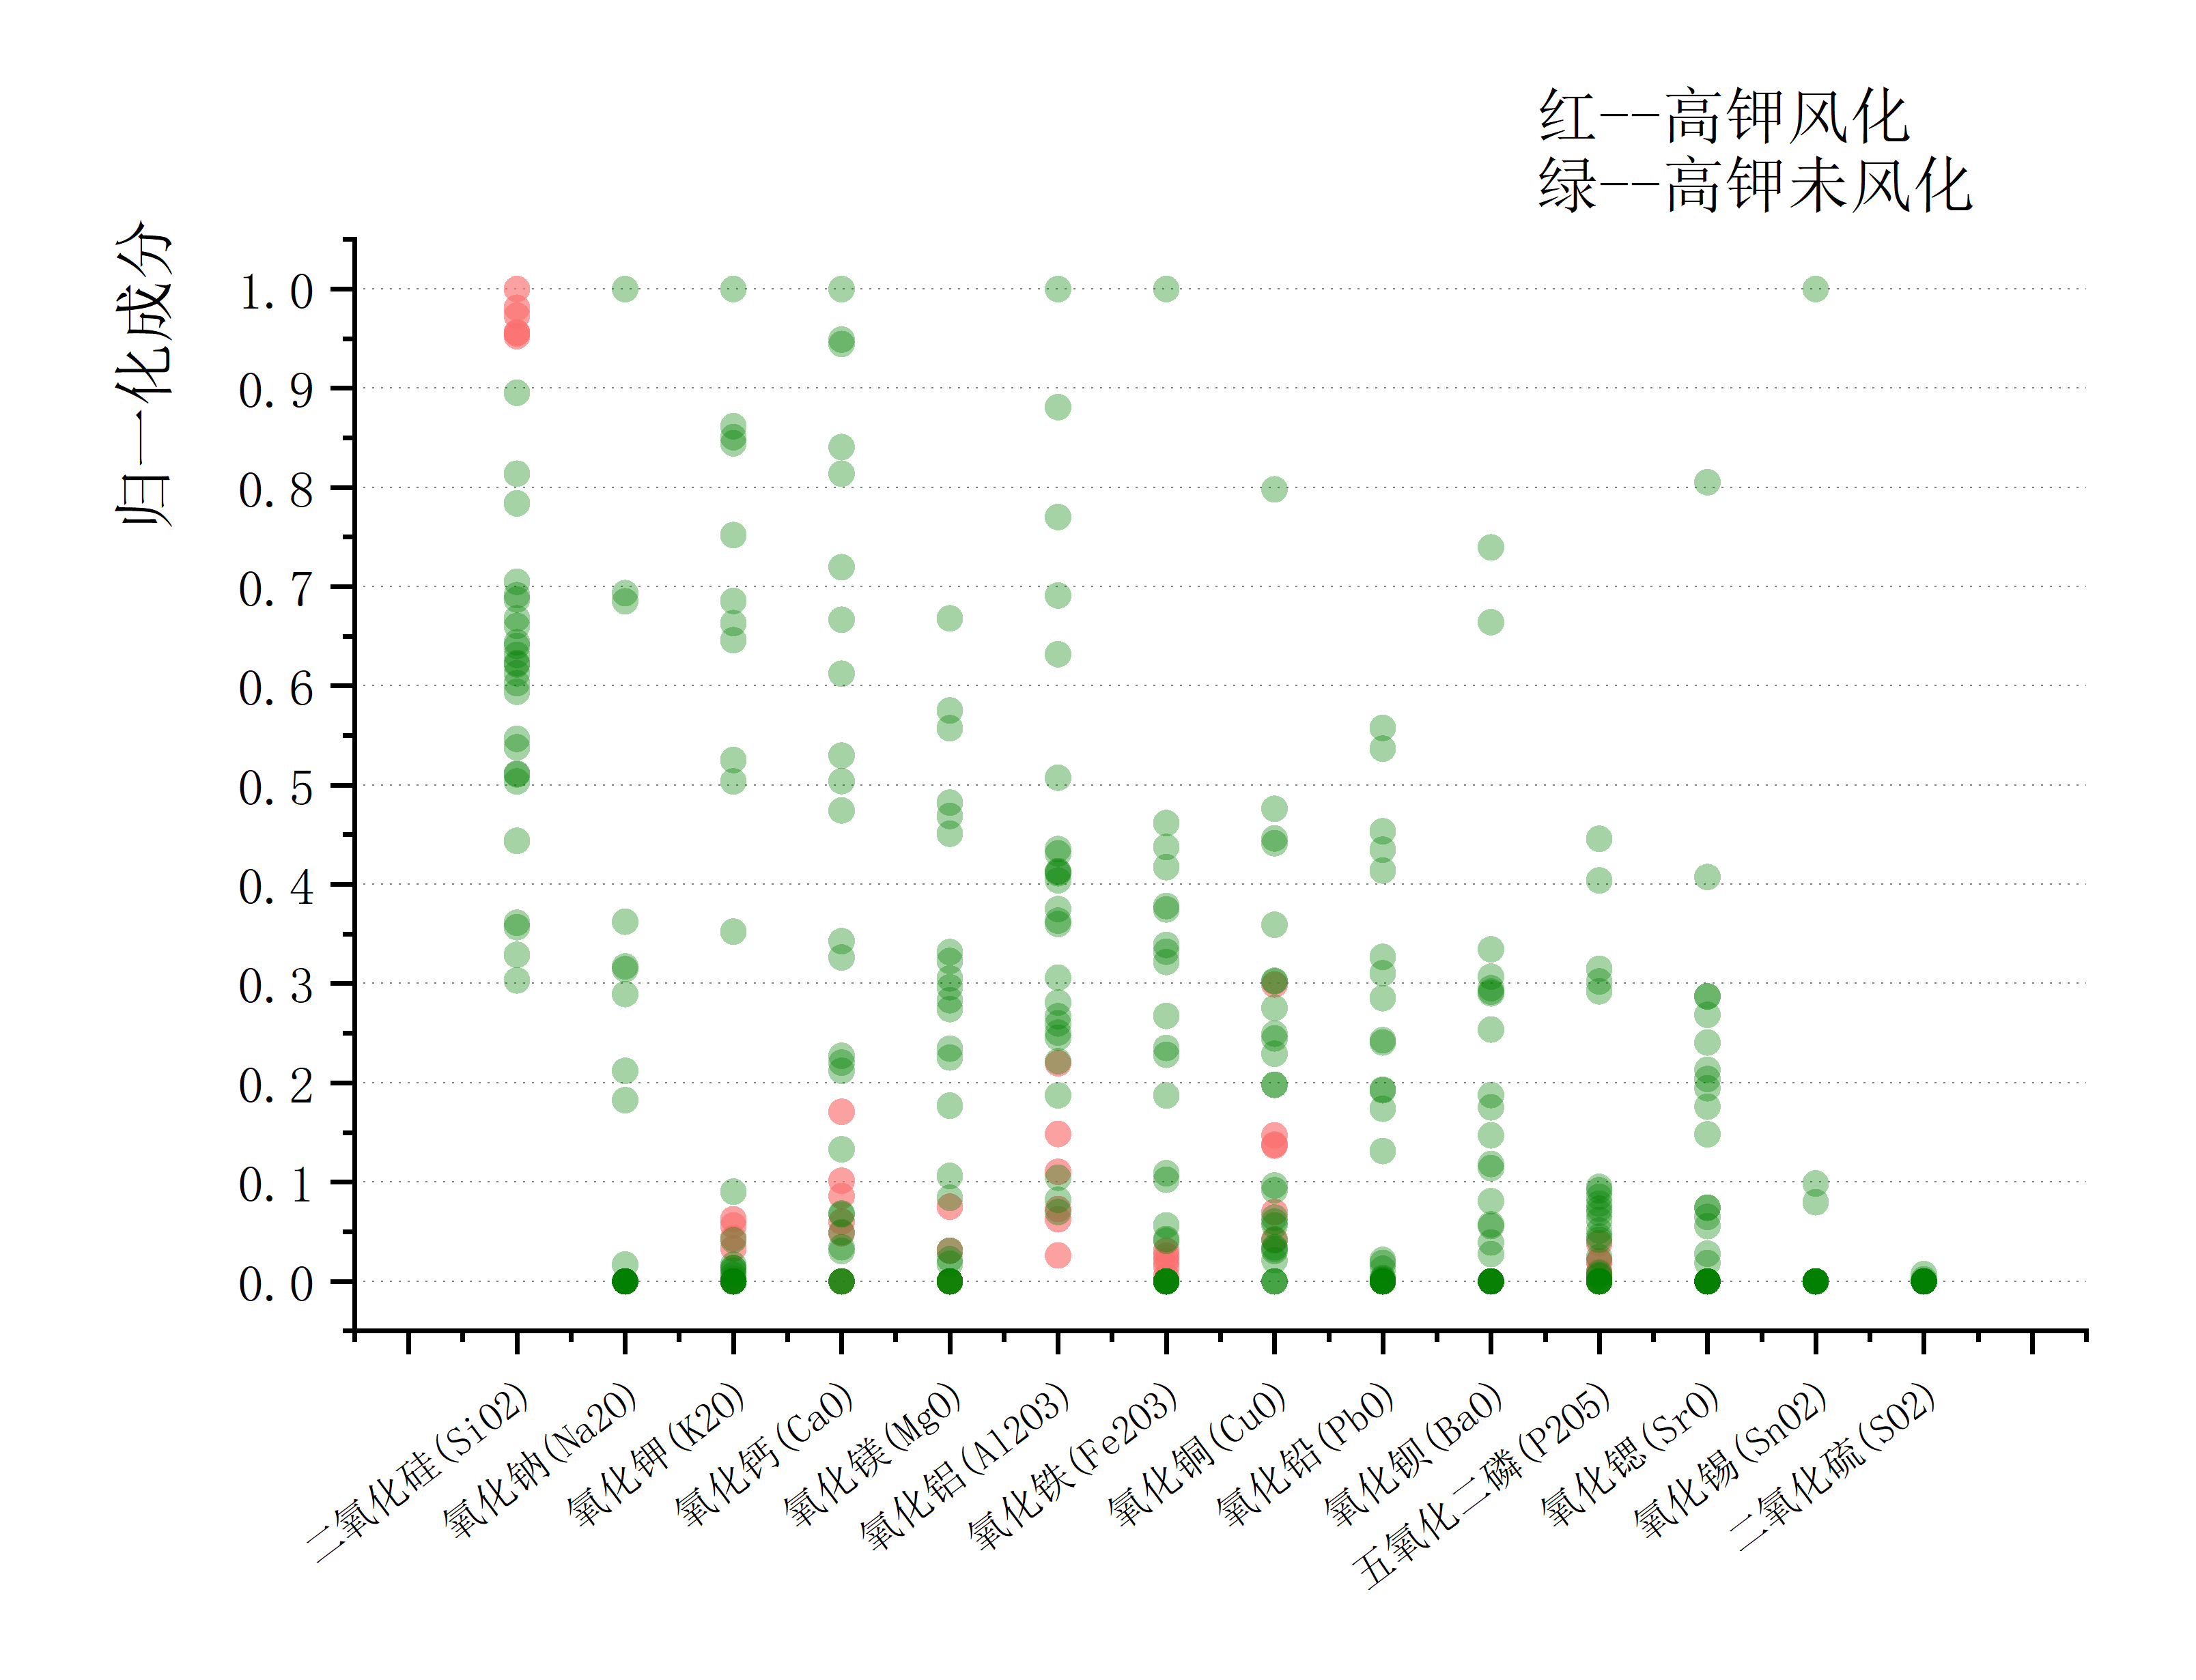
\includegraphics[width=.49\textwidth]{高钾风化与否}
		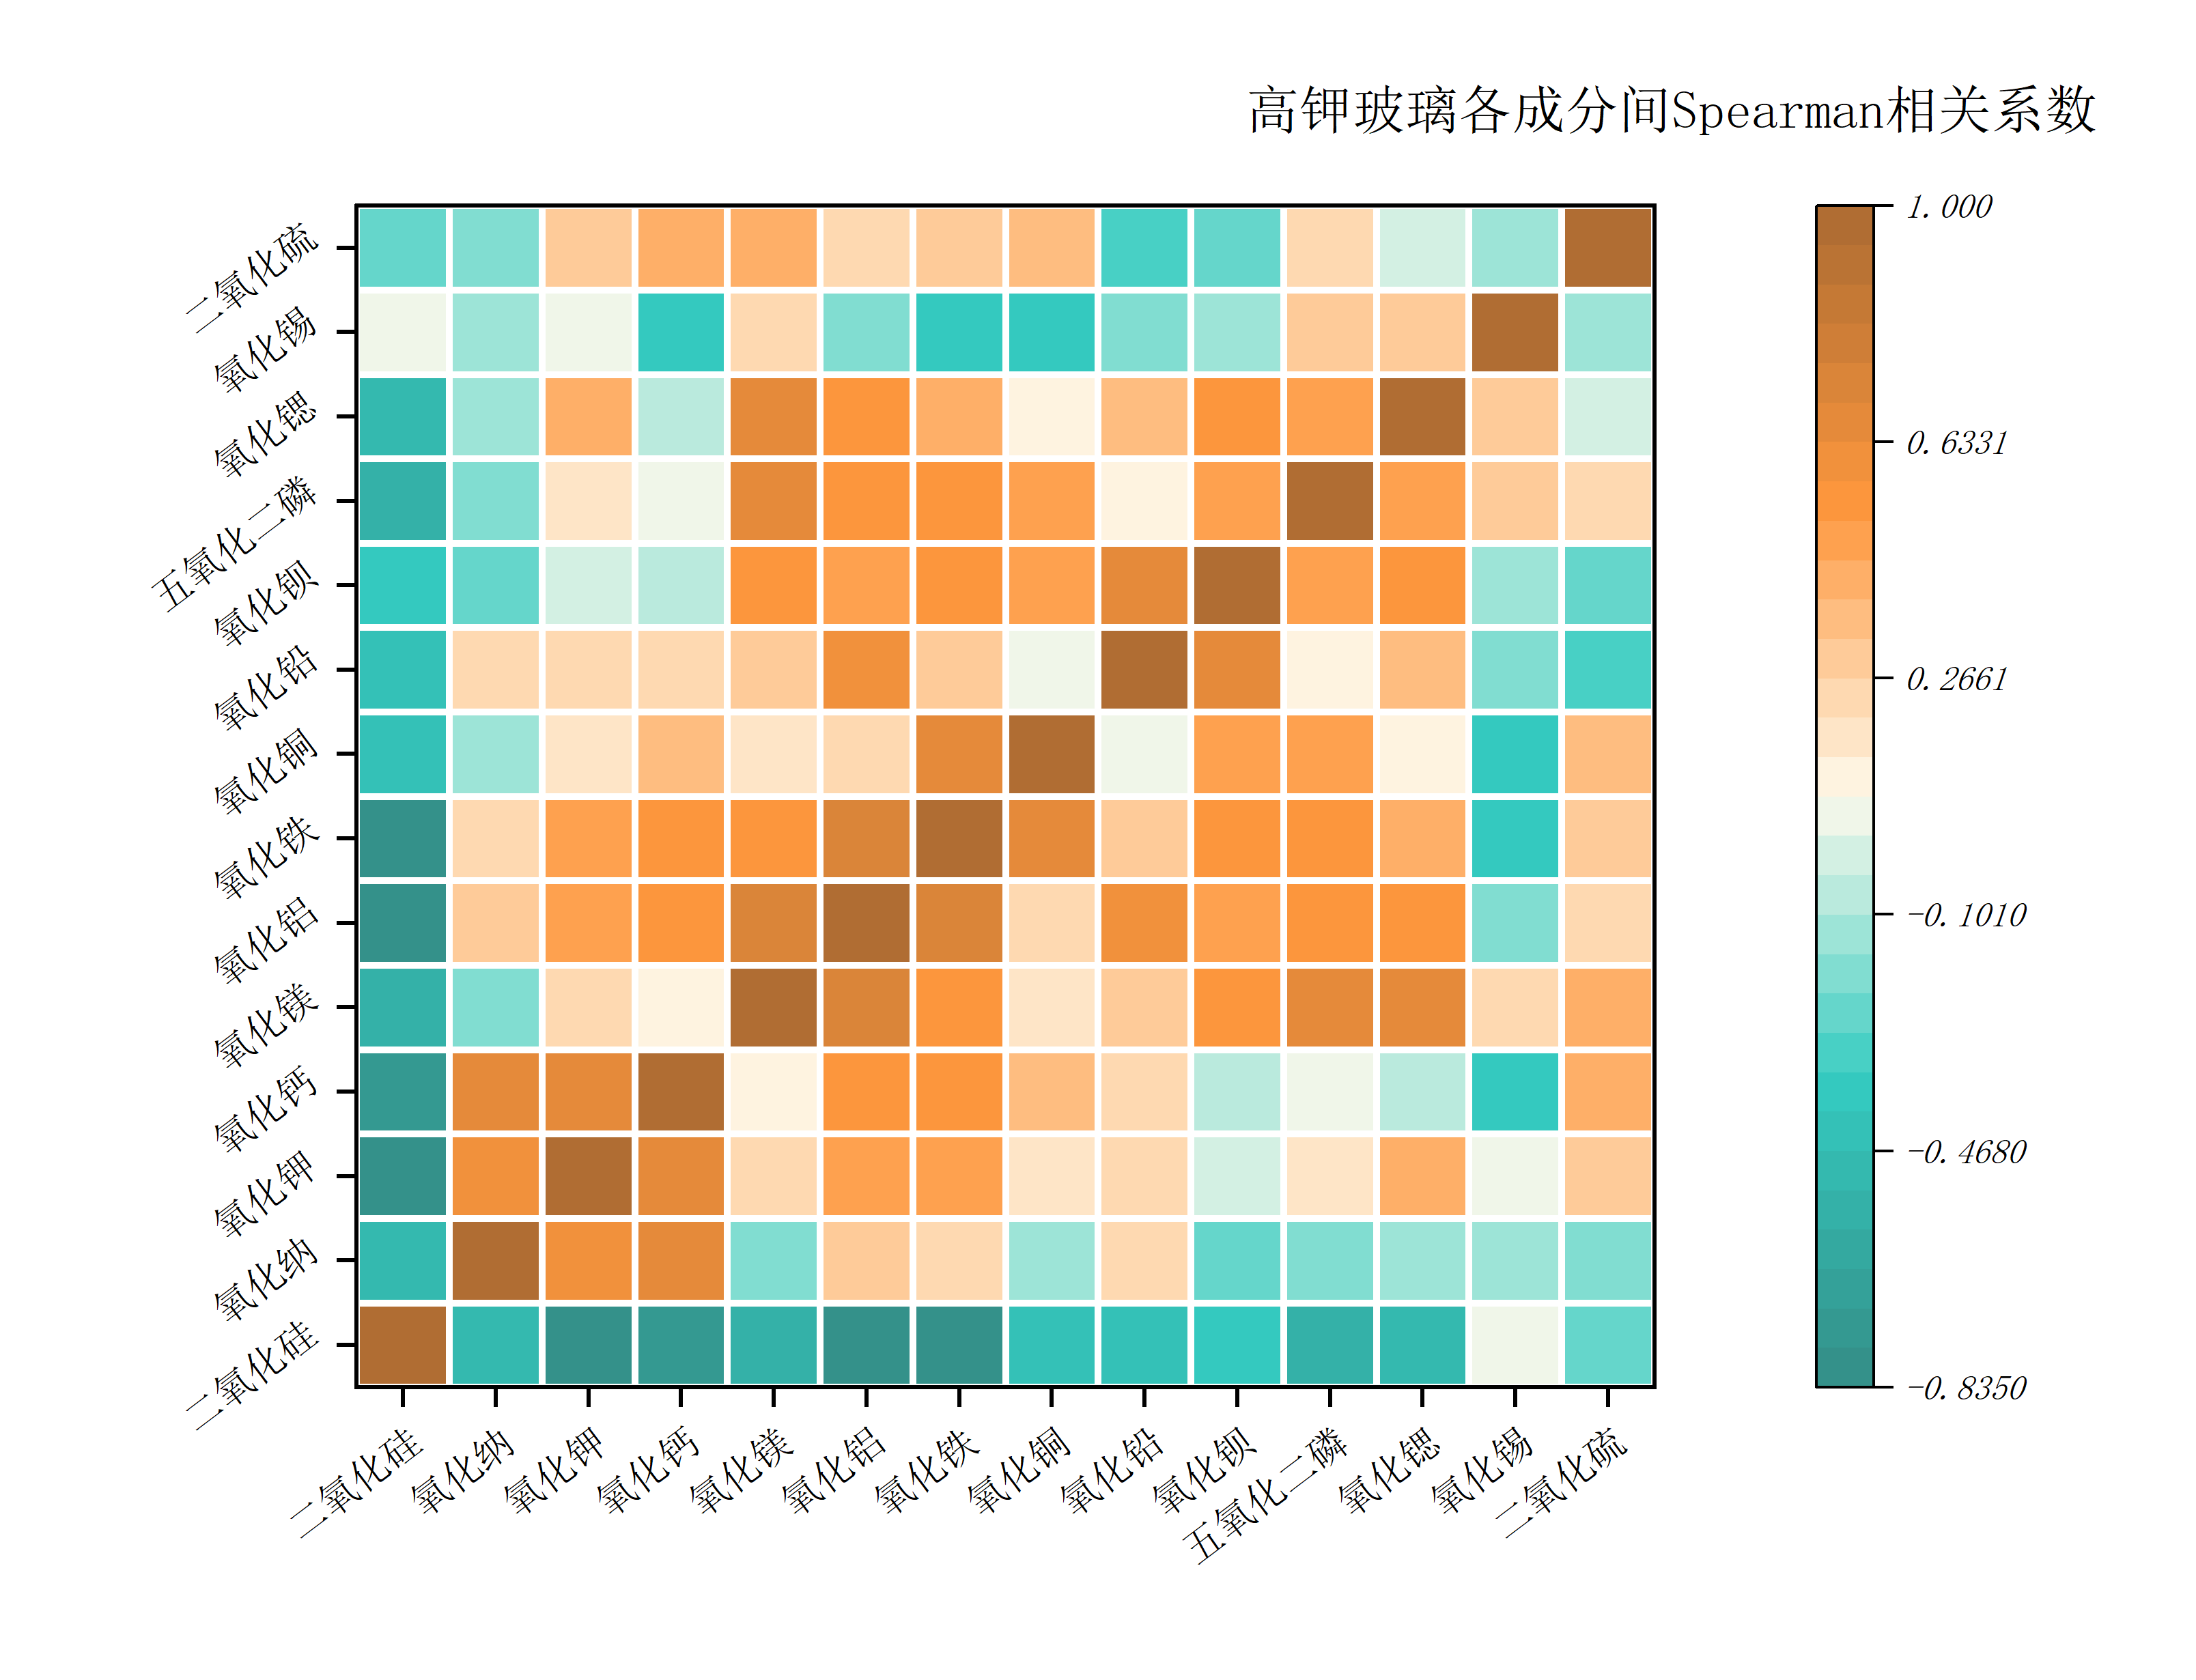
\includegraphics[width=.49\textwidth]{Spearman相关系数}
		\caption{高钾玻璃成分含量散点图(左)与各成分间的Spearman相关系数热力图(右)}
		\label{gjfh}
	\end{figure}
	
	由图\ref{gjfh}(左)可以初步得出,高钾玻璃风化前后对部分化学成分含量有较大影响,其中,对$SiO_{2}$的含量有正向影响、对$K_{2}O$、$CaO$、$MgO$、$Al_{2}O_{3}$、$Fe_{2}O_{3}$、$CuO$、$P_{2}O_{5}$的含量有负向影响。
	
	\item Step2: 计算高钾玻璃各个化学成分的Spearman相关系数。
	
	 定义:X和Y为两组数据,其斯皮尔曼(等级)相关系数为:
	 \[
	 r_{s}=1-\frac{6 \sum_{i=1}^{n} d_{i}^{2}}{n\left(n^{2}-1\right)}
	 \]
	
	 其中,di为Xi和Yi之间的等级差。
	
	若某两种Spearman相关性较大,则可以推测在风化前后这两种化学成分极可能存在某种化学转换关系,结合步骤1,由于众多成分中只有$SiO_{2}$含量明显减少,故主要探究$SiO_{2}$与其他化学成分含量的Spearman系数,将各成分间的Spearman相关系数按颜色划分,得到热力图如图\ref{gjfh}(右)所示。
	
	
以Spearman相关系数0.6为分界,选出与$SiO_{2}$相关性最强的五个化学成分,分别为:$K_{2}O$、$CaO$、$MgO$、$Al_{2}O_{3}$、$Fe_{2}O_{3}$,此结果与步骤一的结果得到了相互印证。
	
	
	\item Step3: 以化学成分含量的比例作为是否风化的依据。
	
	 基于上述分析,构造$SiO_{2}$与其他五个化学成分的比例关系$p_{1}$,$p_{1}$公式如下所示: $$p_{1}=\frac{n(SiO_{2})}{n(K_{2}O)+n(CaO)+n(MgO)+n(Al_{2}O_{3})+n(Fe_{2}O_{3})}$$ 各个高钾玻璃的文物样品的$p_{1}$如表\ref{gjp}所示,由于篇幅关系,仅展示2个风化样品与2个未风化样品的$p_{1}$值,完整表格见附录\ref{app:gjp1}。
	
	
	\begin{table}[!h]
		\centering
		\small 
		\caption{高钾玻璃样品的$p_{1}$示意值}
		\label{gjp}
		\begin{tabular}{@{}cccccccccc@{}}
			\toprule
			\textbf{\begin{tabular}[c]{@{}c@{}}文物\\ 采样点\end{tabular}} & \textbf{类型} & \textbf{\begin{tabular}[c]{@{}c@{}}表面\\ 风化\end{tabular}} & \textbf{\begin{tabular}[c]{@{}c@{}}二氧化硅\\ (SiO2)\end{tabular}} & \textbf{\begin{tabular}[c]{@{}c@{}}氧化钾\\ (K2O)\end{tabular}} & \textbf{\begin{tabular}[c]{@{}c@{}}氧化钙\\ (CaO)\end{tabular}} & \textbf{\begin{tabular}[c]{@{}c@{}}氧化镁\\ (MgO)\end{tabular}} & \textbf{\begin{tabular}[c]{@{}c@{}}氧化铝\\ (Al2O3)\end{tabular}} & \textbf{\begin{tabular}[c]{@{}c@{}}氧化铁\\ (Fe2O3)\end{tabular}} & \textbf{\begin{tabular}[c]{@{}c@{}}高钾的比例\\ (区分风化)\end{tabular}} \\ \midrule
			10                                                        & 高钾          & 风化                                                       & 96.77                                                          & 0.92                                                         & 0.21                                                         & 0.00                                                         & 0.81                                                           & 0.26                                                           & 43.99                                                           \\
			......         &    &    &    &    &    &                       \\
			22                                                        & 高钾          & 风化                                                       & 92.35                                                          & 0.74                                                         & 1.66                                                         & 0.64                                                         & 3.50                                                           & 0.35                                                           & 13.40                                                           \\
			17                                                        & 高钾          & 无风化                                                      & 60.71                                                          & 5.71                                                         & 0.00                                                         & 0.85                                                         & 0.00                                                           & 1.04                                                           & 7.99                                                            \\
			......         &    &    &    &    &    &                       \\
			06部位2                                                     & 高钾          & 无风化                                                      & 59.81                                                          & 7.68                                                         & 5.41                                                         & 1.73                                                         & 10.05                                                          & 6.04                                                           & 1.93                                                            \\ \bottomrule
		\end{tabular}
	\end{table}
	
	
	依照表格信息,可以选取$p_{1}=10.7$作为区分高钾玻璃风化与否的依据。
	
	\item Step4: 总结统计规律。
	
	
	 当高钾玻璃中的$p_{1}=\frac{n(SiO_{2})}{n(K_{2}O)+n(CaO)+n(MgO)+n(Al_{2}O_{3})+n(Fe_{2}O_{3})}$大于10.7时,高钾玻璃出现风化,小于10.7时,高钾玻璃不风化。
	
\end{itemize}


接着对铅钡玻璃进行分析,铅钡玻璃的分析流程与高钾玻璃类似,首先得出铅钡玻璃的风化前后化学成分含量归一化后的散点图,如图\ref{qbfh}(左)所示


\begin{figure}[!h]
	\centering
	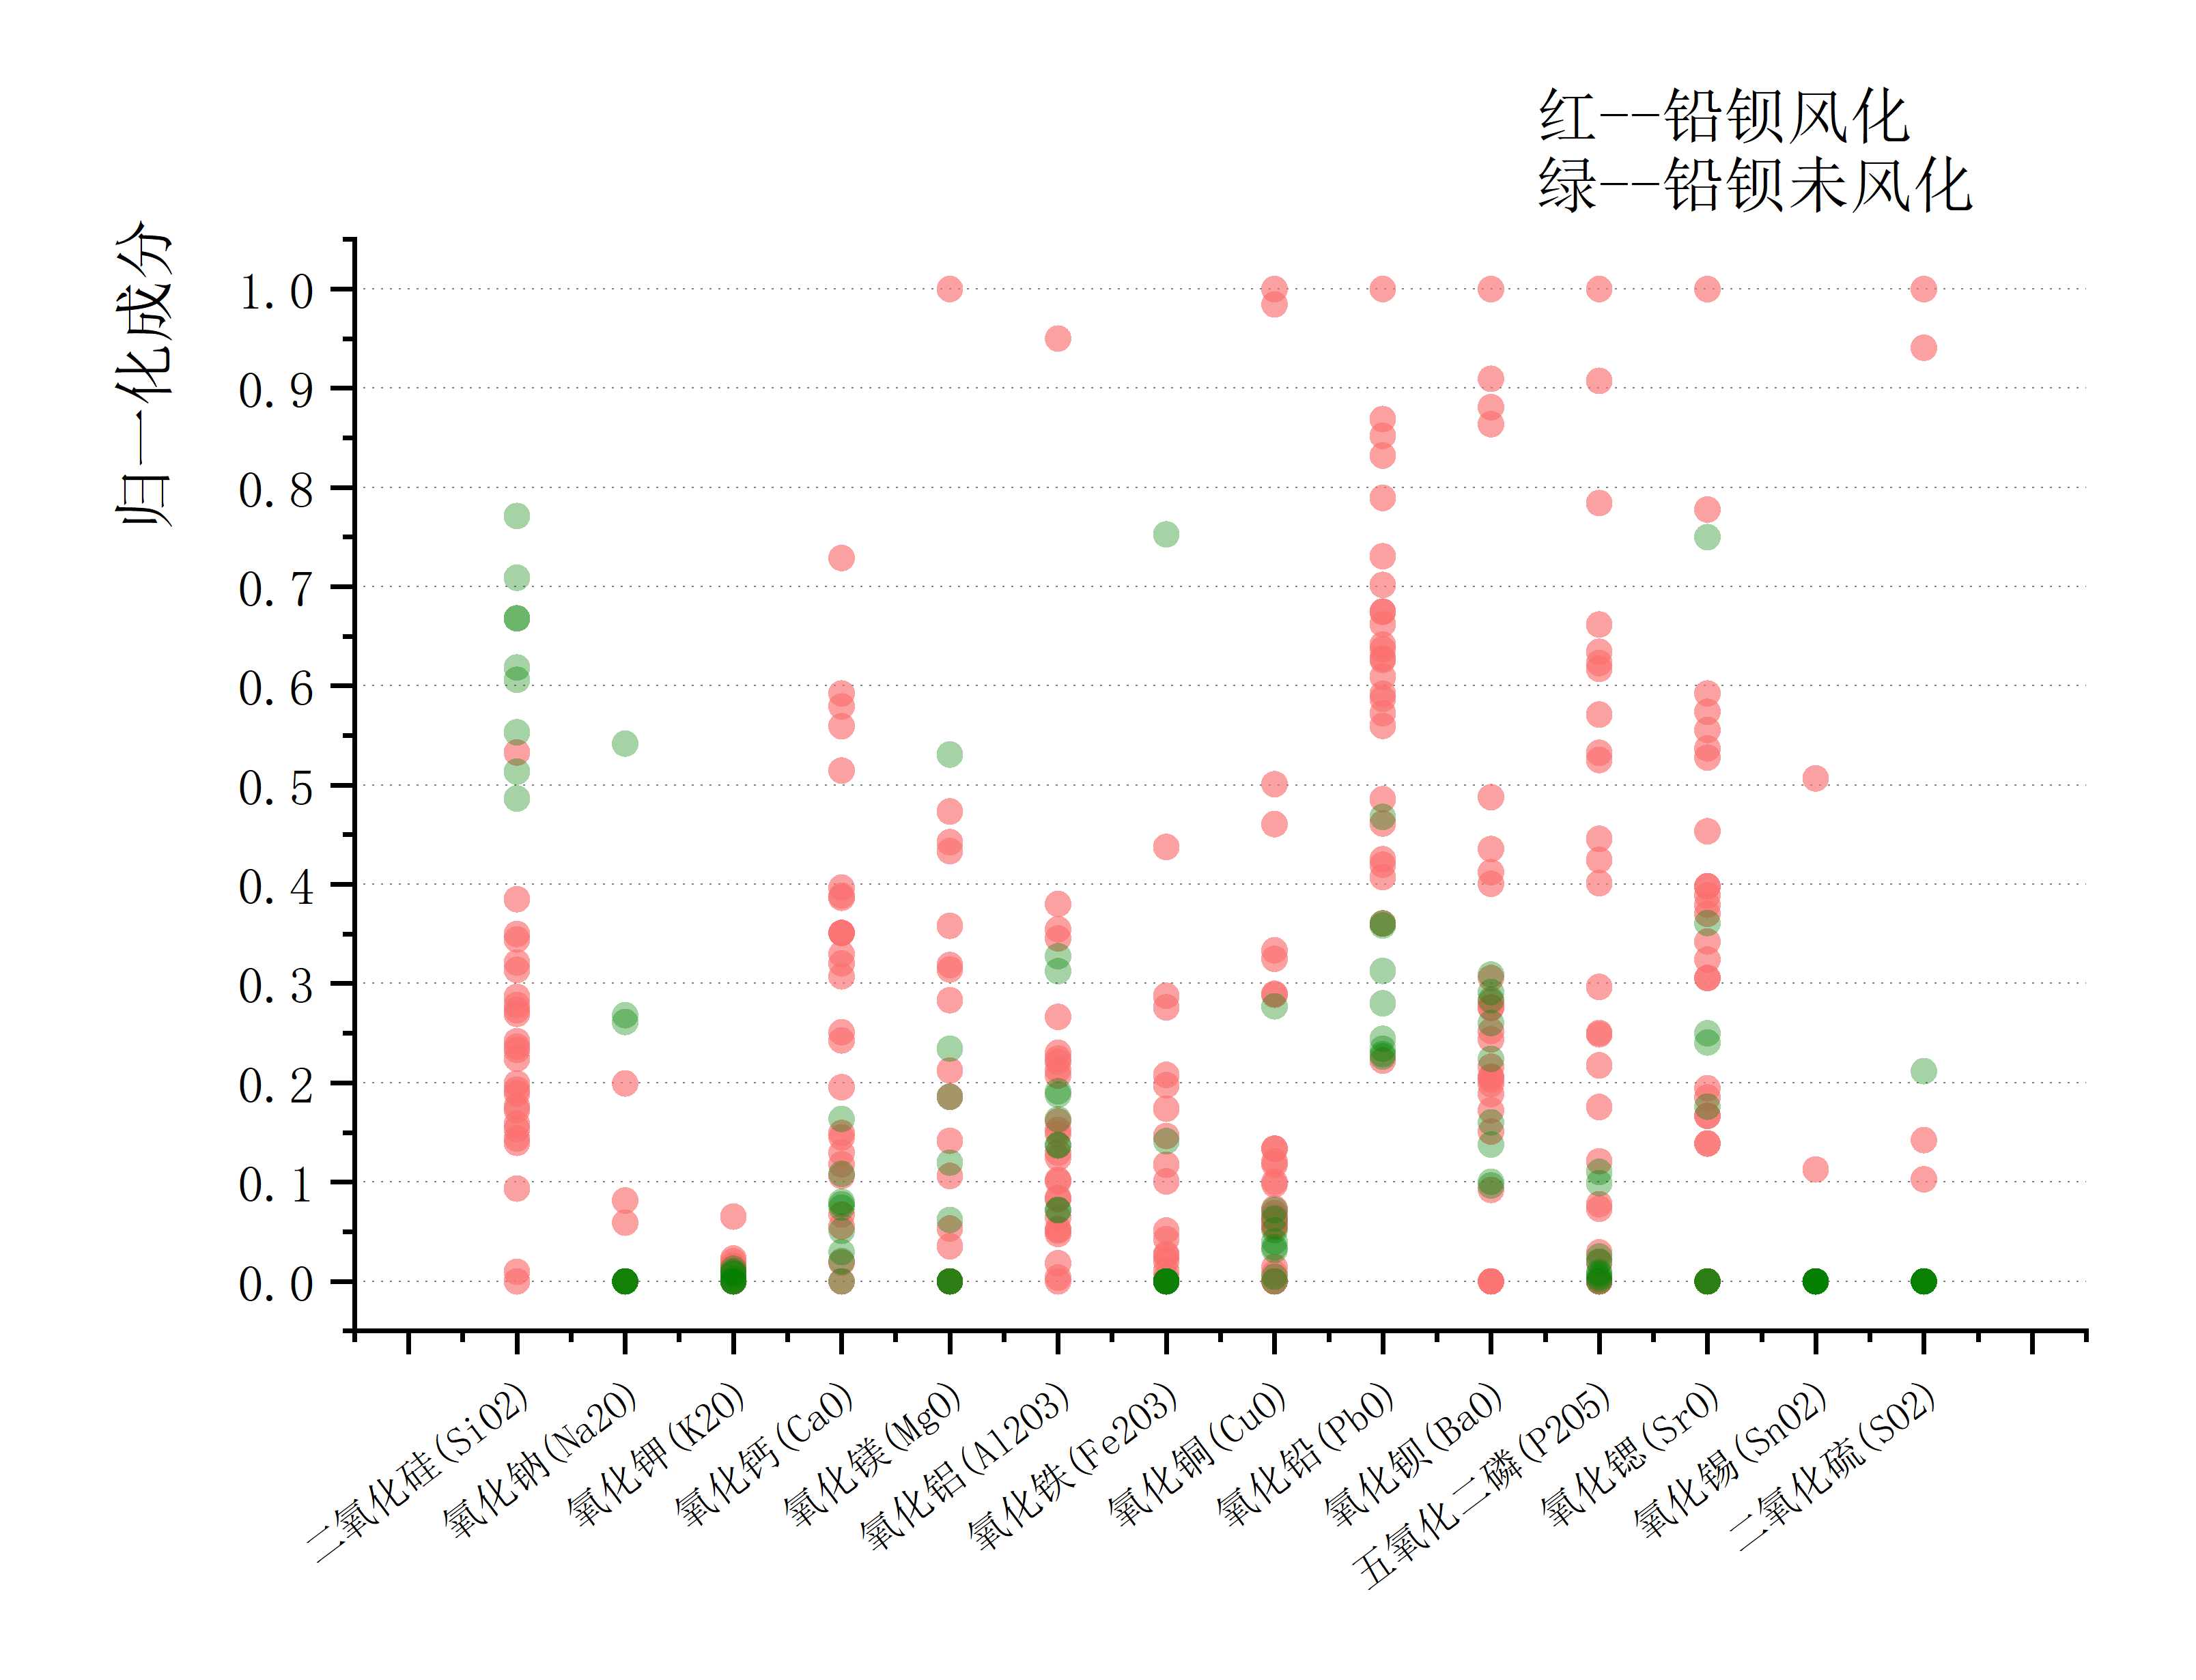
\includegraphics[width=.49\textwidth]{铅钡风化与否}
	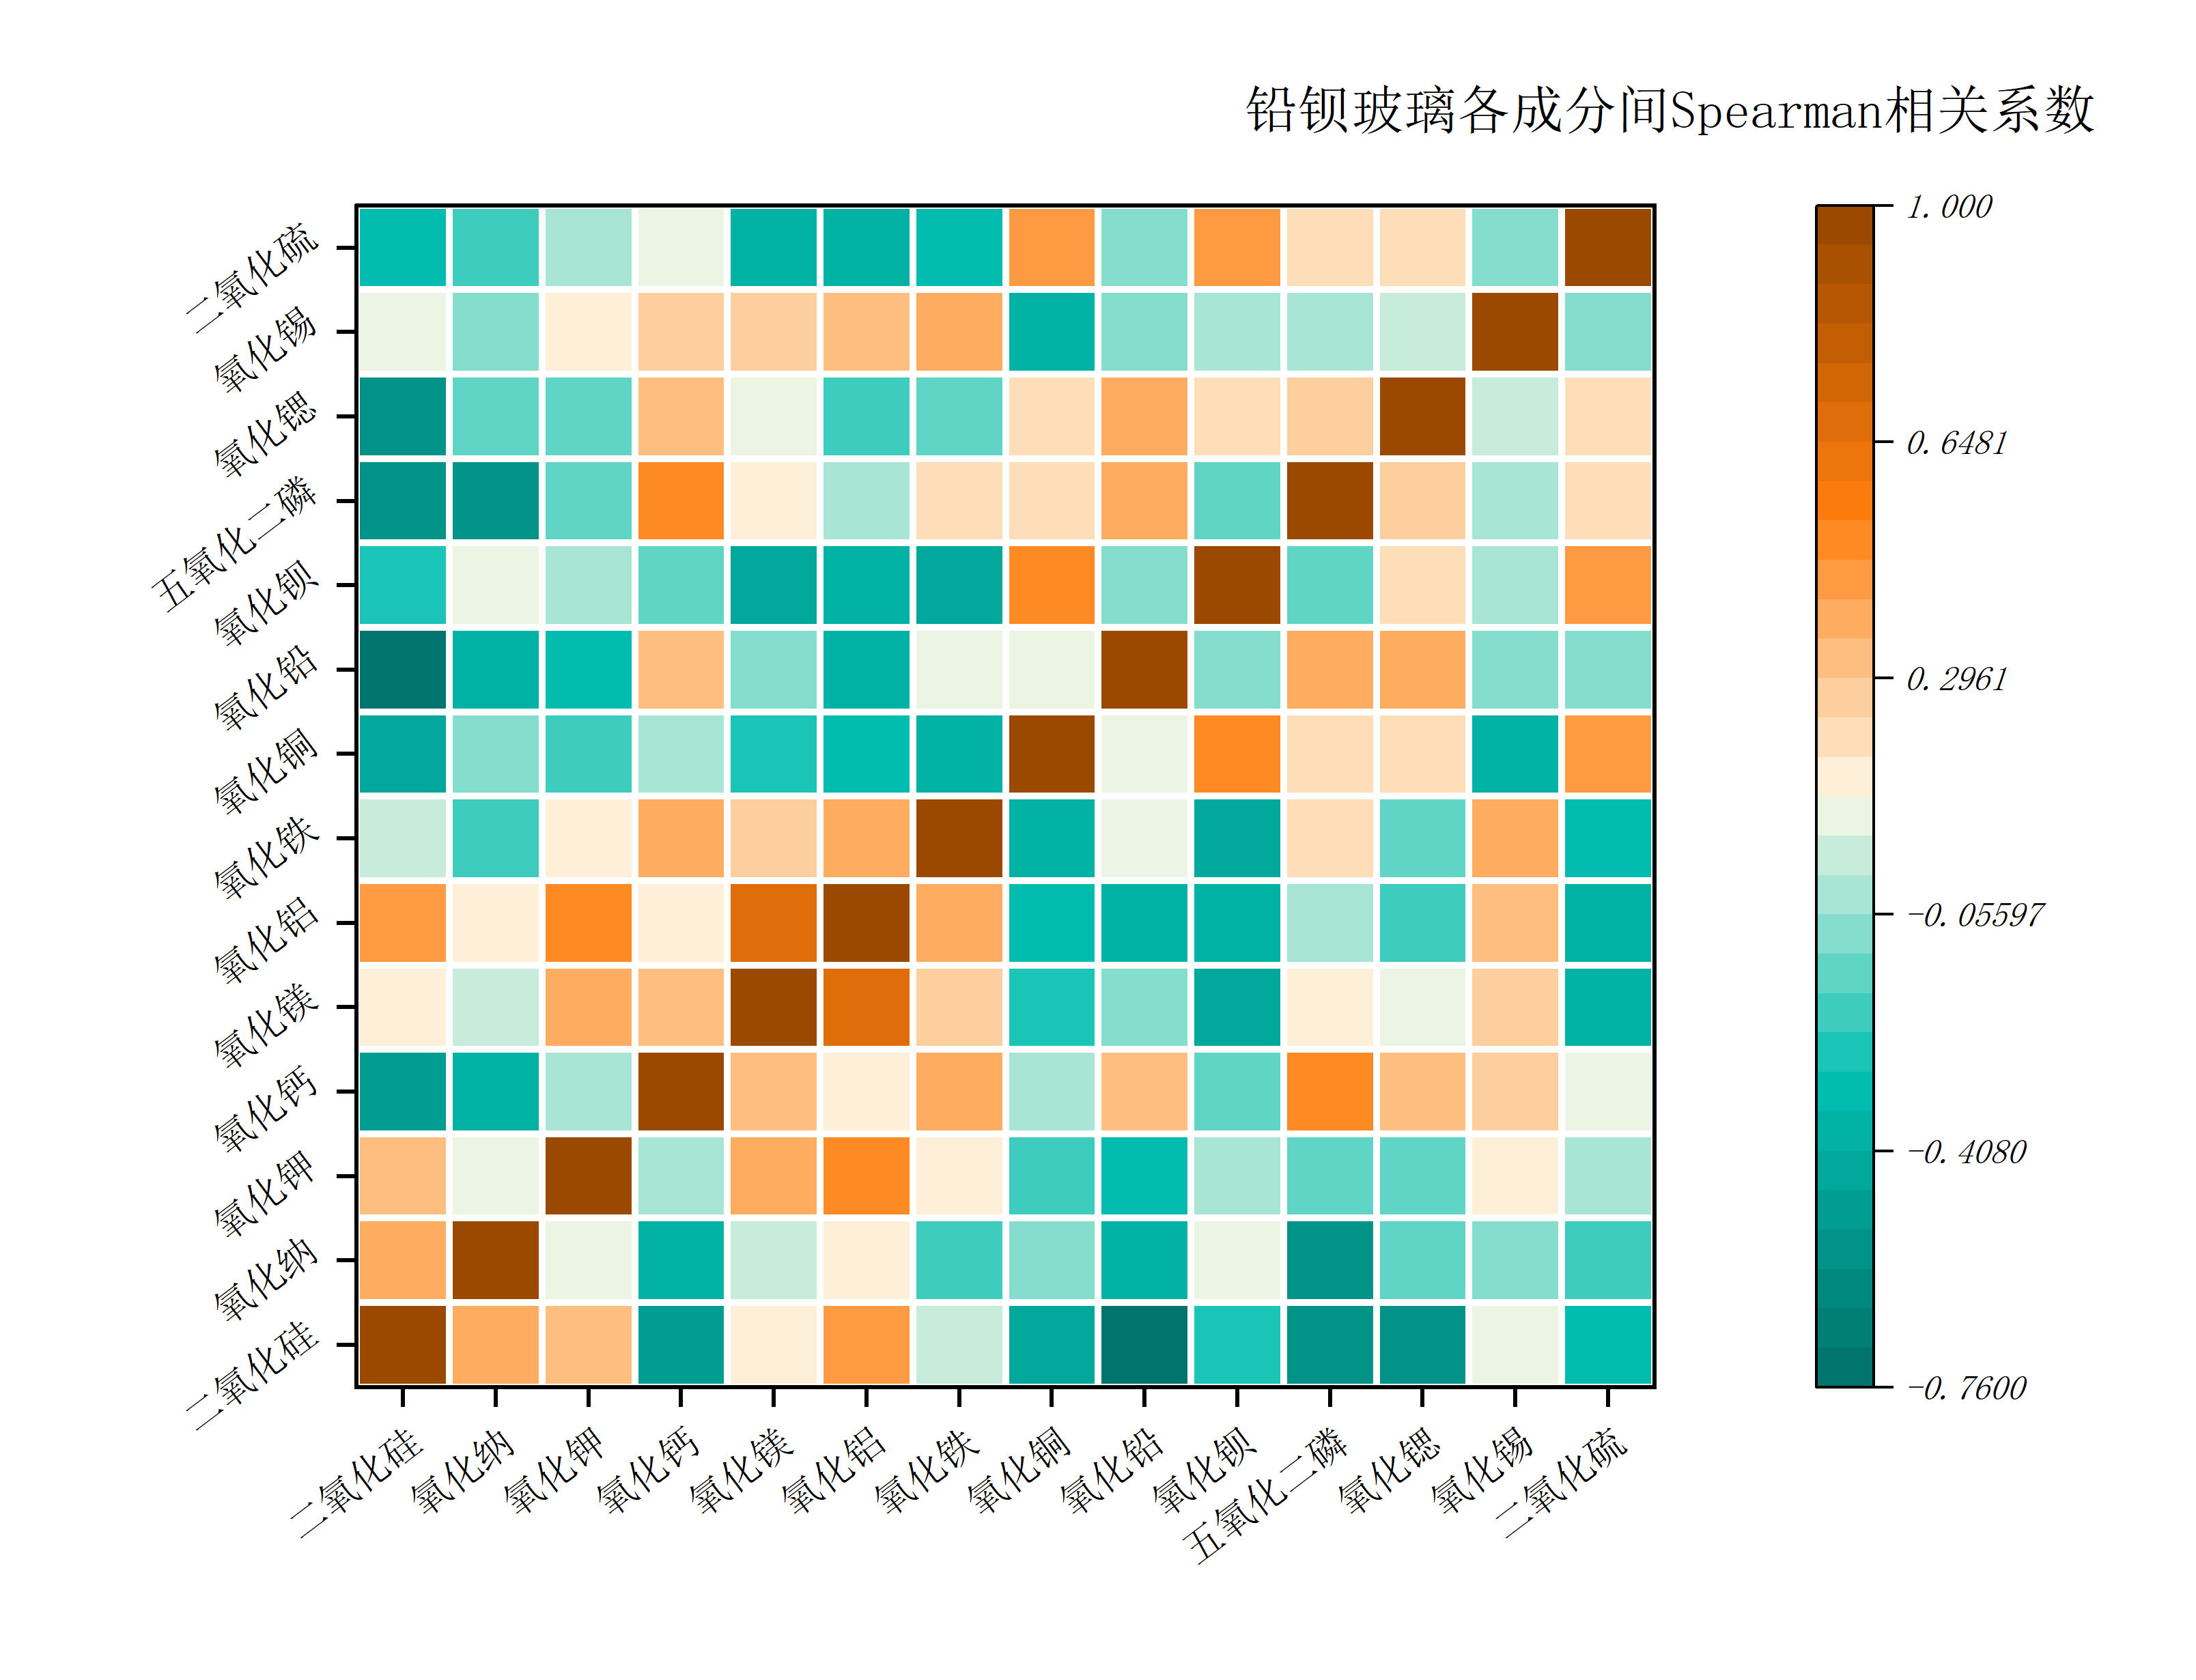
\includegraphics[width=.49\textwidth]{Spearman相关系数2}
	\caption{铅钡玻璃成分含量散点图(左)与各成分间的Spearman相关系数热力图(右)}
	\label{qbfh}
\end{figure}


从图中除了能分析出风化后$SiO_{2}$含量减少之外,较难分析铅钡玻璃中风化前后化学成分的变化,故需要求解Spearman相关系数进行进一步观察,可视化Spearman相关系数热力图如图\ref{qbfh}(右)所示。


从中提取出与$SiO_{2}$相关性较强的$PbO$、$CuO$、$BaO$三个化学成分,同样地,构造$SiO_{2}$与这三个化学成分含量的比例关系值$p_{2}$,即 $$p_{2}=\frac{n(SiO_{2})}{n(PbO)+n(CuO)+n(BaO)}$$


各个铅钡玻璃的文物样品的$p_{2}$如表\ref{qbfhp}所示,由于篇幅关系,仅展示2个风化样品与2个未风化样品的$p_{2}$值,完整表格见附录\ref{app:qbp2}。

\begin{table}[!h]
	\centering
	\small
	\caption{铅钡玻璃样品的$p_{2}$示意值}
	\label{qbfhp}
	\begin{tabular}{@{}cccccccc@{}}
	\toprule
	\textbf{\begin{tabular}[c]{@{}c@{}}文物\\ 采样点\end{tabular}} & \textbf{类型} & \textbf{\begin{tabular}[c]{@{}c@{}}表面\\ 风化\end{tabular}} & \textbf{\begin{tabular}[c]{@{}c@{}}二氧化硅\\ (SiO2)\end{tabular}} & \textbf{\begin{tabular}[c]{@{}c@{}}氧化铜\\ (CuO)\end{tabular}} & \textbf{\begin{tabular}[c]{@{}c@{}}氧化铅\\ (PbO)\end{tabular}} & \textbf{\begin{tabular}[c]{@{}c@{}}氧化钡\\ (BaO)\end{tabular}} & \textbf{\begin{tabular}[c]{@{}c@{}}铅钡的比例\\ (区分风化)\end{tabular}} \\ \midrule
	26严重风化点                                                   & 铅钡          & 风化                                                       & 3.72                                                           & 3.60                                                         & 29.92                                                        & 35.45                                                        & 0.05                                                            \\
	......  &  &  &  &  &  &                                \\
	11                                                        & 铅钡          & 风化                                                       & 33.59                                                          & 4.93                                                         & 25.39                                                        & 14.61                                                        & 0.75                                                            \\
	50未风化点                                                    & 铅钡          & \begin{tabular}[c]{@{}c@{}}风化\\ (实际无风化)\end{tabular}     & 45.02                                                          & 0.70                                                         & 30.61                                                        & 6.22                                                         & 1.20                                                            \\
	......  &  &  &  &  &  &                                \\
	29未风化点                                                    & 铅钡          & 无风化                                                      & 63.30                                                          & 0.74                                                         & 12.31                                                        & 2.03                                                         & 4.20                                                            \\ \bottomrule
\end{tabular}
\end{table}


依照表\ref{qbfhp}信息,选取$p_{2}=0.70$作为分解规律,得到如下结论:


当铅钡玻璃中的$p_{2}=\frac{n(SiO_{2})}{n(PbO)+n(CuO)+n(BaO)}$大于0.7时,高钾玻璃出现风化,小于0.7时,高钾玻璃不风化。此分类结果不完全准确,有3个样本不符合此规律,分别是11,36和48。


\subsection{基于反向传播变换的线性逻辑回归的预测模型}
预测风化前化学成分含量之前,先将其中的化学成分分为三类,如图\ref{sanlei}所示。

\begin{figure}[!h]
	\centering
	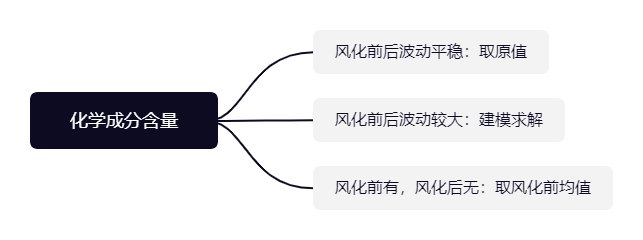
\includegraphics[width=.69\textwidth]{sanlei}
	\caption{三类化学成分}
	\label{sanlei}
\end{figure}

模型算法流程如图\ref{liucheng}所示。

\begin{figure}[!h]
	\centering
	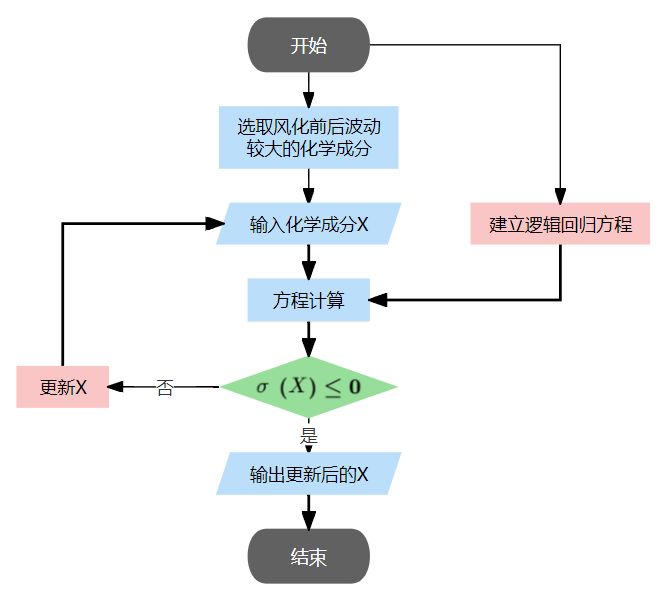
\includegraphics[width=.65\textwidth]{liucheng}
	\caption{模型算法流程图}
	\label{liucheng}
\end{figure}

本节首先对高钾玻璃风化前的化学成分进行预测,预测过程如下:

\subsubsection{选取特征(化学成分含量)}

特征量的选取主要基于图\ref{gjfh}(左),由上述分析可知,风化前后只对$SiO_{2}$、$K_{2}O$、$CaO$、$MgO$、$Al_{2}O_{3}$、$Fe_{2}O_{3}$、$CuO$的含量有显著影响,故将这七个化学成分含量视为系统输入的特征值。为了方便表达,选取的七个特征值依次用$x_{1}$、$x_{2}$......$x_{7}$表示。 对于其他含量,风化前后波动较平稳的$P_{2}O_{5}$使用原值近似预测值,风化后消失的元素使用风化前元素的平均值近似预测值。


\subsubsection{建立线性逻辑回归方程}

\begin{itemize}
	\item step1: 构建一般方程。
	
	
	引入sigmoid函数,sigmoid有两个特性,第一个是其函数值在趋于正无穷或负无穷时,函数趋近平滑状态,第二个是sigmoid函数输出范围为(0,1),因此,sigmoid函数经常用于二分类问题,其函数表达式如下所示: $$\sigma(z)=\frac{1}{1+\mathrm{e}^{-z}}$$ 为了建立输出与特征的关系,考虑使用$x_{i}$的线性表达来替代$z$,则z可以被表达为 $$z=w_{0}+w_{1}\cdot x_{1} + w_{2}\cdot x_{2}+....+w_{7} \cdot x_{7} = \vec{w} ^{T} \cdot \vec{x}$$ 具体到本问题中,$\vec{w}$、$\vec{x}$的维度是8,且$\vec{x}$的第一个元素是1,将与$w_{0}$相乘,形成偏置。此时,线性逻辑回归的表达式就可以表达为: $$\sigma_{w}(x)=\frac{1}{1+\mathrm{e}^{-\vec{w} ^{T} \cdot \vec{x}}}$$
	\item step2: 构建逻辑回归的损失函数。
	
	
	单个样本点的损失值记为$cost$,构造如下所示的$cost$的表达式。 
	\[
	\operatorname{cost}\left(\sigma_{w}(x), y\right)=\left\{\begin{array}{r}
		-\log \left(\sigma_{w}(x)\right) \text { if } y=1 \\
		-\log \left(1-\sigma_{w}(x)\right) \text { if } y=0
	\end{array}\right.
	\] 
	
	构建cost表达式后,就可以构建出逻辑回归的损失函数
	\[\begin{aligned} J(\theta) &=\frac{1}{m} \sum_{i=1}^{m} \operatorname{cost}\left(\sigma_{w}\left(x^{(i)}\right), y^{(i)}\right) \ \\ &=-\frac{1}{m}\left[\sum_{i=1}^{m} y^{(i)} \log \sigma_{w}\left(x^{(i)}\right)+\left(1-y^{(i)}\right) \log \left(1-\sigma_{w}\left(x^{(i)}\right)\right)\right] \end{aligned}
	\]
	\item step3: 代入数据,训练模型。
	
	代入高钾玻璃的数据,标记风化为1,无风化为0,进行训练,通过对损失函数求偏导更新参数,最终建立逻辑回归方程。
	
	\item step4: 方程准确度的验证。
	
	如图\ref{chazhi},可视化方程预测值与实际值的差距
	
	\begin{figure}[!h]
		\centering
		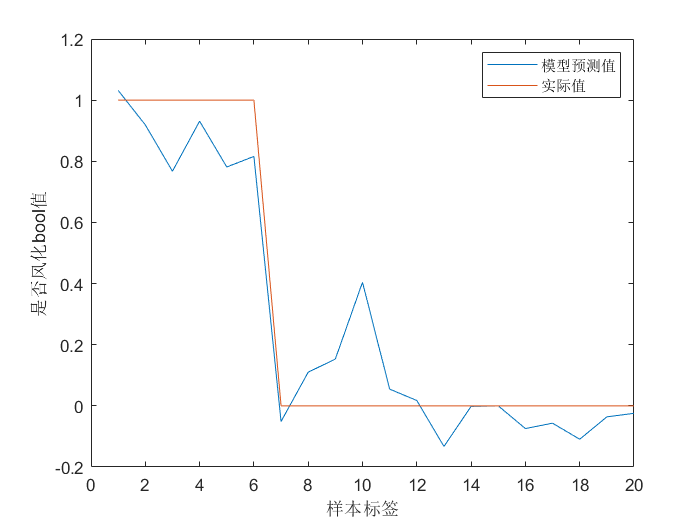
\includegraphics[width=.69\textwidth]{chazhi}
		\caption{方程预测值与实际值的风化bool值}
		\label{chazhi}
	\end{figure}
	
	方程的具体参数如表\ref{canshu}所示。
	
	\begin{table}[!h]
		\centering
		\small
		\caption{模型方程的具体参数}
		\label{canshu}
		\begin{tabular}{|c|ccccccc|}
			\hline
			\textbf{权重系数(coef)}    & \multicolumn{1}{c|}{0.03059} & \multicolumn{1}{c|}{0.00604} & \multicolumn{1}{c|}{-0.043613} & \multicolumn{1}{c|}{-0.115602} & \multicolumn{1}{c|}{0.03004} & \multicolumn{1}{c|}{0.17706} & -0.18683 \\ \hline
			\textbf{偏置(intercept)} & \multicolumn{7}{c|}{-1.99501}                                                                                                                                                                          \\ \hline
			\textbf{准确率}           & \multicolumn{7}{c|}{0.82063}                                                                                                                                                                           \\ \hline
		\end{tabular}
	\end{table}
	
\end{itemize}

\subsubsection{化学成分含量的反向传播}

本文通过按照一定比例依次调整风化后样本的化学成分含量,直到逻辑回归的方程判定由“1”变为“0”为止,达到预测风化前化学成分含量的效果。由于是对多组化学变量同时调整,故需要设定不同的调整幅度,此幅度由不同化学成分含量风化前后的均值的变化量之比决定。幅度比如下所示: $$\bigtriangleup \mu_{CuO}:\bigtriangleup \mu_{Fe_{2}O_{3}}:\bigtriangleup \mu_{Al_{2}O_{3}}:\bigtriangleup \mu_{MgO}:\bigtriangleup \mu_{CaO}:\bigtriangleup \mu_{K_{2}O}:\bigtriangleup \mu_{SiO_{2}} \\
=1:2.166:5.587:1.213:5.209:11.814:-37.913$$ 


本算法的伪代码如下所示:

\begin{python}
	Init mu,alpha       #初始化上述比例系数行向量,alpha为幅值系数,本例设为0.005
	while :
	x = x*(1+alpha*mu) #更新x,每个x的更新幅度由mu决定
	if (f(x)==0):
	break            #若经过逻辑回归判定为0,未风化,则跳出循环
\end{python}

更新后,得到六组风化后的高钾玻璃的化学成分的预测量,如表\ref{gjyc}所示,结果同样将展示在附录\ref{app:yucel}中。


\begin{table}[!h]
	\centering
	\tiny
	\caption{风化后高钾玻璃化学成分的预测量}
	\label{gjyc}
\begin{tabular}{@{}ccccccccccccccc@{}}
	\toprule
	\textbf{\begin{tabular}[c]{@{}c@{}}文物\\ 采样点\end{tabular}} & \textbf{\begin{tabular}[c]{@{}c@{}}二氧化硅\\ (SiO2)\end{tabular}} & \textbf{\begin{tabular}[c]{@{}c@{}}氧化钠\\ (Na2O)\end{tabular}} & \textbf{\begin{tabular}[c]{@{}c@{}}氧化钾\\ (K2O)\end{tabular}} & \textbf{\begin{tabular}[c]{@{}c@{}}氧化钙\\ (CaO)\end{tabular}} & \textbf{\begin{tabular}[c]{@{}c@{}}氧化镁\\ (MgO)\end{tabular}} & \textbf{\begin{tabular}[c]{@{}c@{}}氧化铝\\ (Al2O3)\end{tabular}} & \textbf{\begin{tabular}[c]{@{}c@{}}氧化铁\\ (Fe2O3)\end{tabular}} & \textbf{\begin{tabular}[c]{@{}c@{}}氧化铜\\ (CuO)\end{tabular}} & \textbf{\begin{tabular}[c]{@{}c@{}}氧化铅\\ (PbO)\end{tabular}} & \textbf{\begin{tabular}[c]{@{}c@{}}氧化钡\\ (BaO)\end{tabular}} & \textbf{\begin{tabular}[c]{@{}c@{}}五氧化二磷\\ (P2O5)\end{tabular}} & \textbf{\begin{tabular}[c]{@{}c@{}}氧化锶\\ (SrO)\end{tabular}} & \textbf{\begin{tabular}[c]{@{}c@{}}氧化锡\\ (SnO2)\end{tabular}} & \textbf{\begin{tabular}[c]{@{}c@{}}二氧化硫\\ (SO2)\end{tabular}} \\ \midrule
	\textbf{12}                                               & 67.549                                                         & 0.976                                                         & 9.951                                                        & 4.472                                                        & 0.862                                                        & 5.431                                                          & 1.830                                                          & 2.360                                                        & 0.380                                                        & 0.513                                                        & 0.150                                                           & 0.036                                                        & 0.169                                                         & 0.087                                                         \\
	\textbf{22}                                               & 71.648                                                         & 0.976                                                         & 9.312                                                        & 5.361                                                        & 1.523                                                        & 7.470                                                          & 1.889                                                          & 1.236                                                        & 0.380                                                        & 0.513                                                        & 0.210                                                           & 0.036                                                        & 0.169                                                         & 0.087                                                         \\
	\textbf{9}                                                & 72.596                                                         & 0.976                                                         & 8.994                                                        & 4.321                                                        & 0.868                                                        & 5.289                                                          & 1.862                                                          & 2.267                                                        & 0.380                                                        & 0.513                                                        & 0.350                                                           & 0.036                                                        & 0.169                                                         & 0.087                                                         \\
	\textbf{27}                                               & 70.284                                                         & 0.976                                                         & 8.373                                                        & 4.657                                                        & 0.540                                                        & 2.510                                                          & 1.740                                                          & 2.254                                                        & 0.380                                                        & 0.513                                                        & 0.360                                                           & 0.036                                                        & 0.169                                                         & 0.087                                                         \\
	\textbf{7}                                                & 70.183                                                         & 0.976                                                         & 8.394                                                        & 4.783                                                        & 0.864                                                        & 5.947                                                          & 1.709                                                          & 3.954                                                        & 0.380                                                        & 0.513                                                        & 0.610                                                           & 0.036                                                        & 0.169                                                         & 0.087                                                         \\
	\textbf{10}                                               & 75.371                                                         & 0.976                                                         & 9.343                                                        & 3.912                                                        & 0.862                                                        & 4.779                                                          & 1.800                                                          & 1.550                                                        & 0.380                                                        & 0.513                                                        & 0.000                                                           & 0.036                                                        & 0.169                                                         & 0.087                                                         \\ \bottomrule
\end{tabular}
\end{table}


对于铅钡玻璃的化学成分的预测量,采用同样的预测方式,由于铅钡玻璃各个成分变化均较大,故选取铅钡的除了二氧化硫的十三个化学成分进行训练,构建铅钡玻璃的逻辑回归模型,最终反向更新化学成分含量,得到铅钡玻璃风化前化学成分的预测量,具体预测值见附录\ref{app:qbycl}。


\section{问题二模型的建立与求解}
\subsection{高钾、铅钡玻璃分类规律的描述性统计分析}

本文首先将预处理好的附件表二中玻璃类别与14种化学组成成分的关系用散点图进行可视化分析, 得到“所有玻璃文物类别与成分关系图”、“风化玻璃文物类别与成分关系图”和“未风化玻璃文物类别与成分关系图” 对类别与成分之间的关系进行直观的定性分析; 随后计算类别与单个化学成分之间的$spearman$相关系数 对类别与成分之间的关系做定量分析。

\subsubsection{统计规律的定性分析}
所有玻璃文物类别与成分关系散点图如图\ref{ztgx}所示。

\begin{figure}[!h]
	\centering
	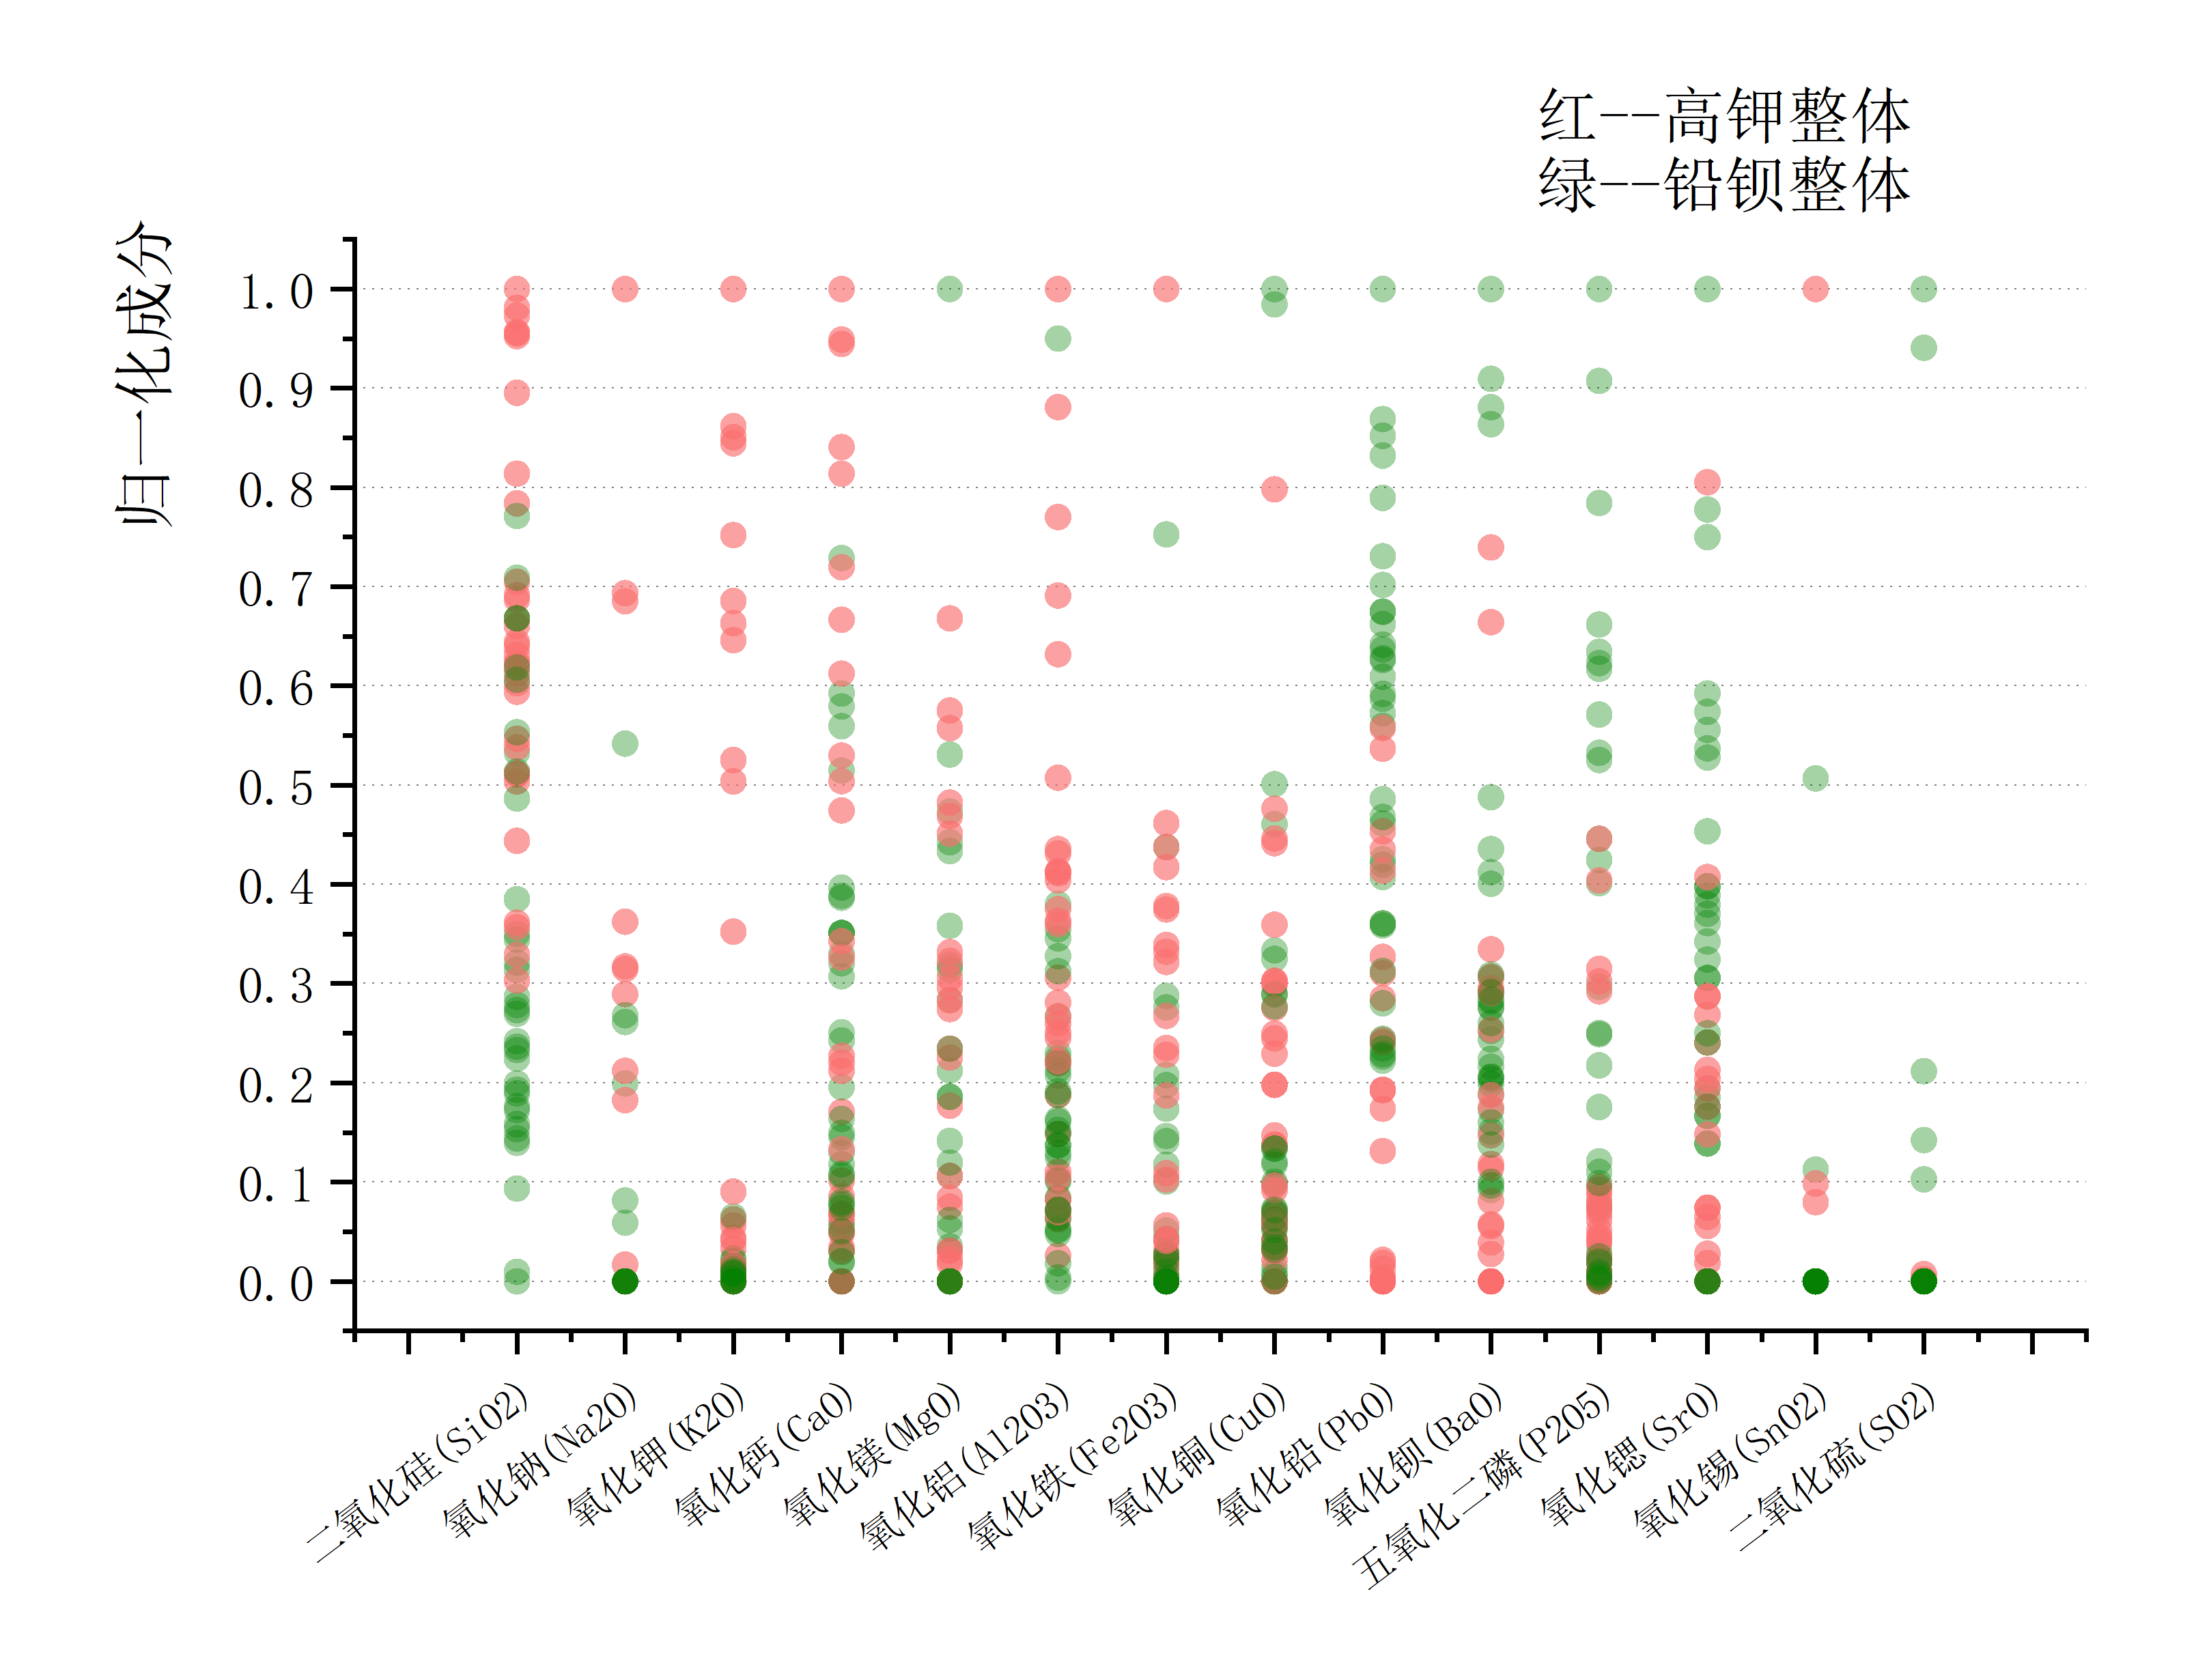
\includegraphics[width=.69\textwidth]{类别成分分析}
	\caption{玻璃文物整体的类别与成分关系散点图}
	\label{ztgx}
\end{figure}

从图中可以看出:高钾玻璃的氧化钾含量基本上高于比铅钡玻璃,且有较明显的分界线; 而高钾玻璃的氧化铅含量普遍低于铅钡玻璃。 在二氧化硅含量方面,高钾玻璃的含量大多偏高,而铅钡玻璃的含量则相对中等,整体趋势高钾玻璃的二氧化硅含量更高, 但二者含量的交集也不少。


将预处理后的表二数据按照风化与否分别画出玻璃类别与化学成分含量的散点图如图\ref{fhgx}所示。

\begin{figure}[!h]
	\centering
	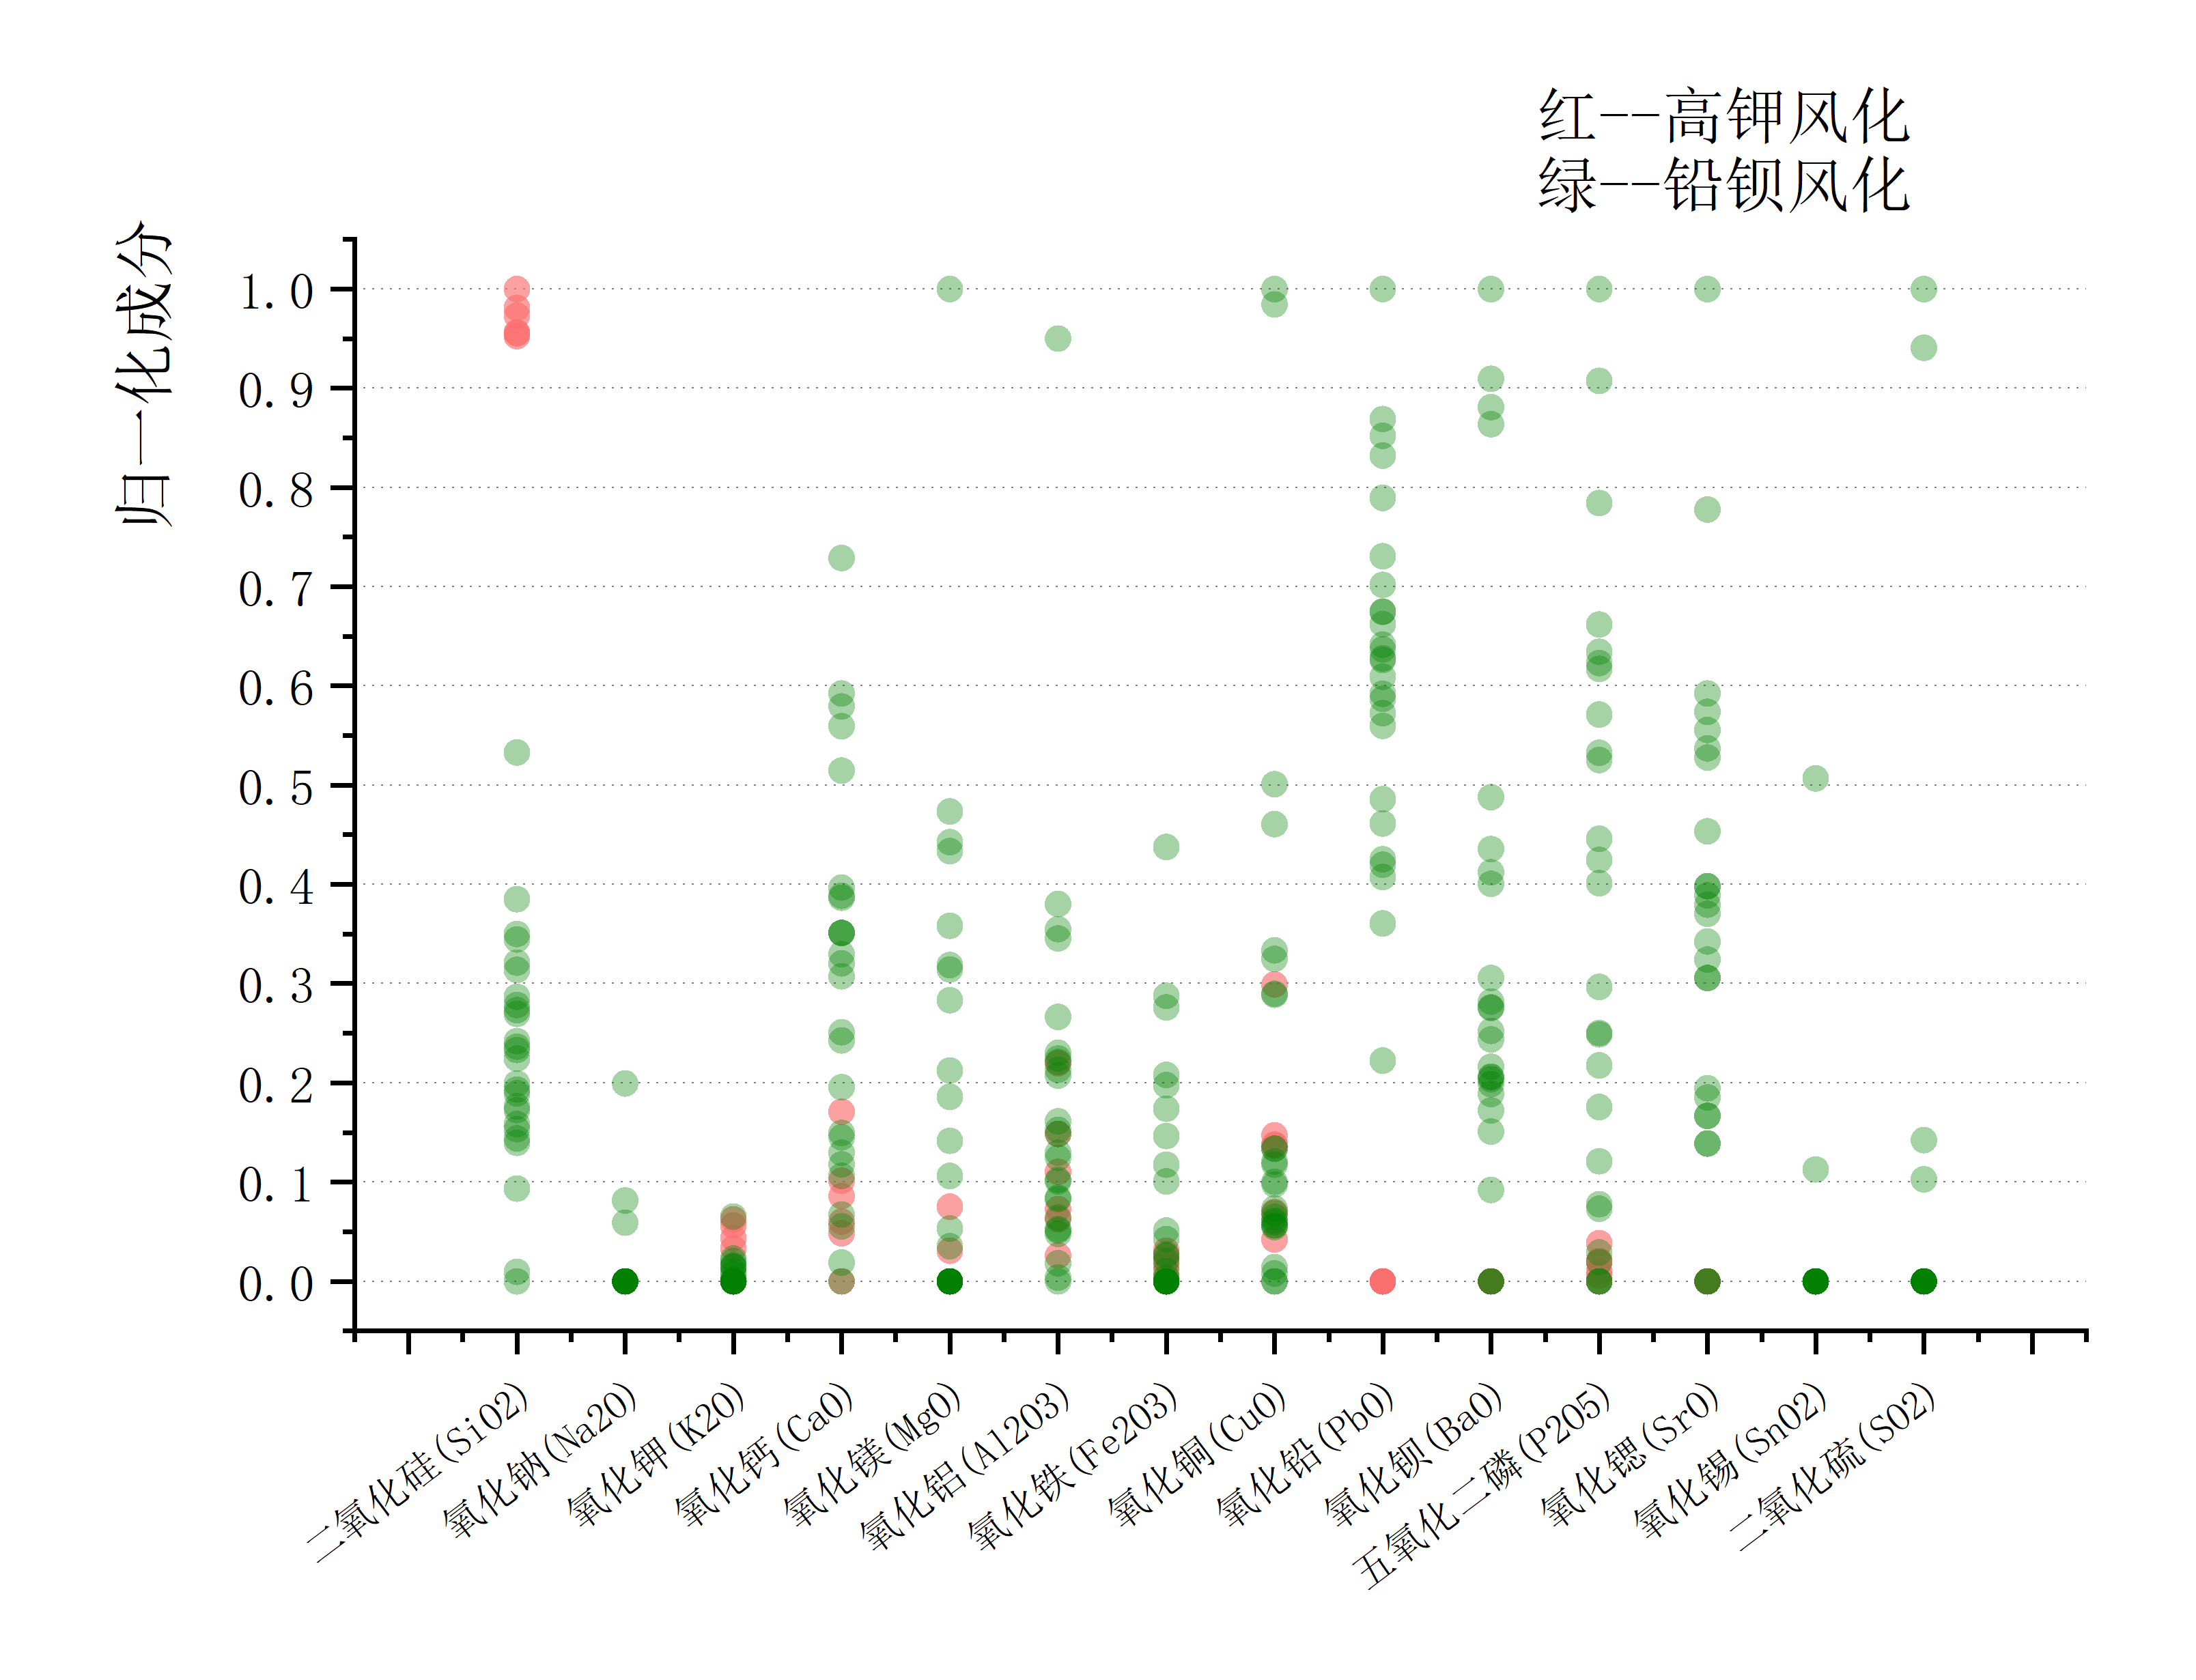
\includegraphics[width=.49\textwidth]{风化类别分析}
	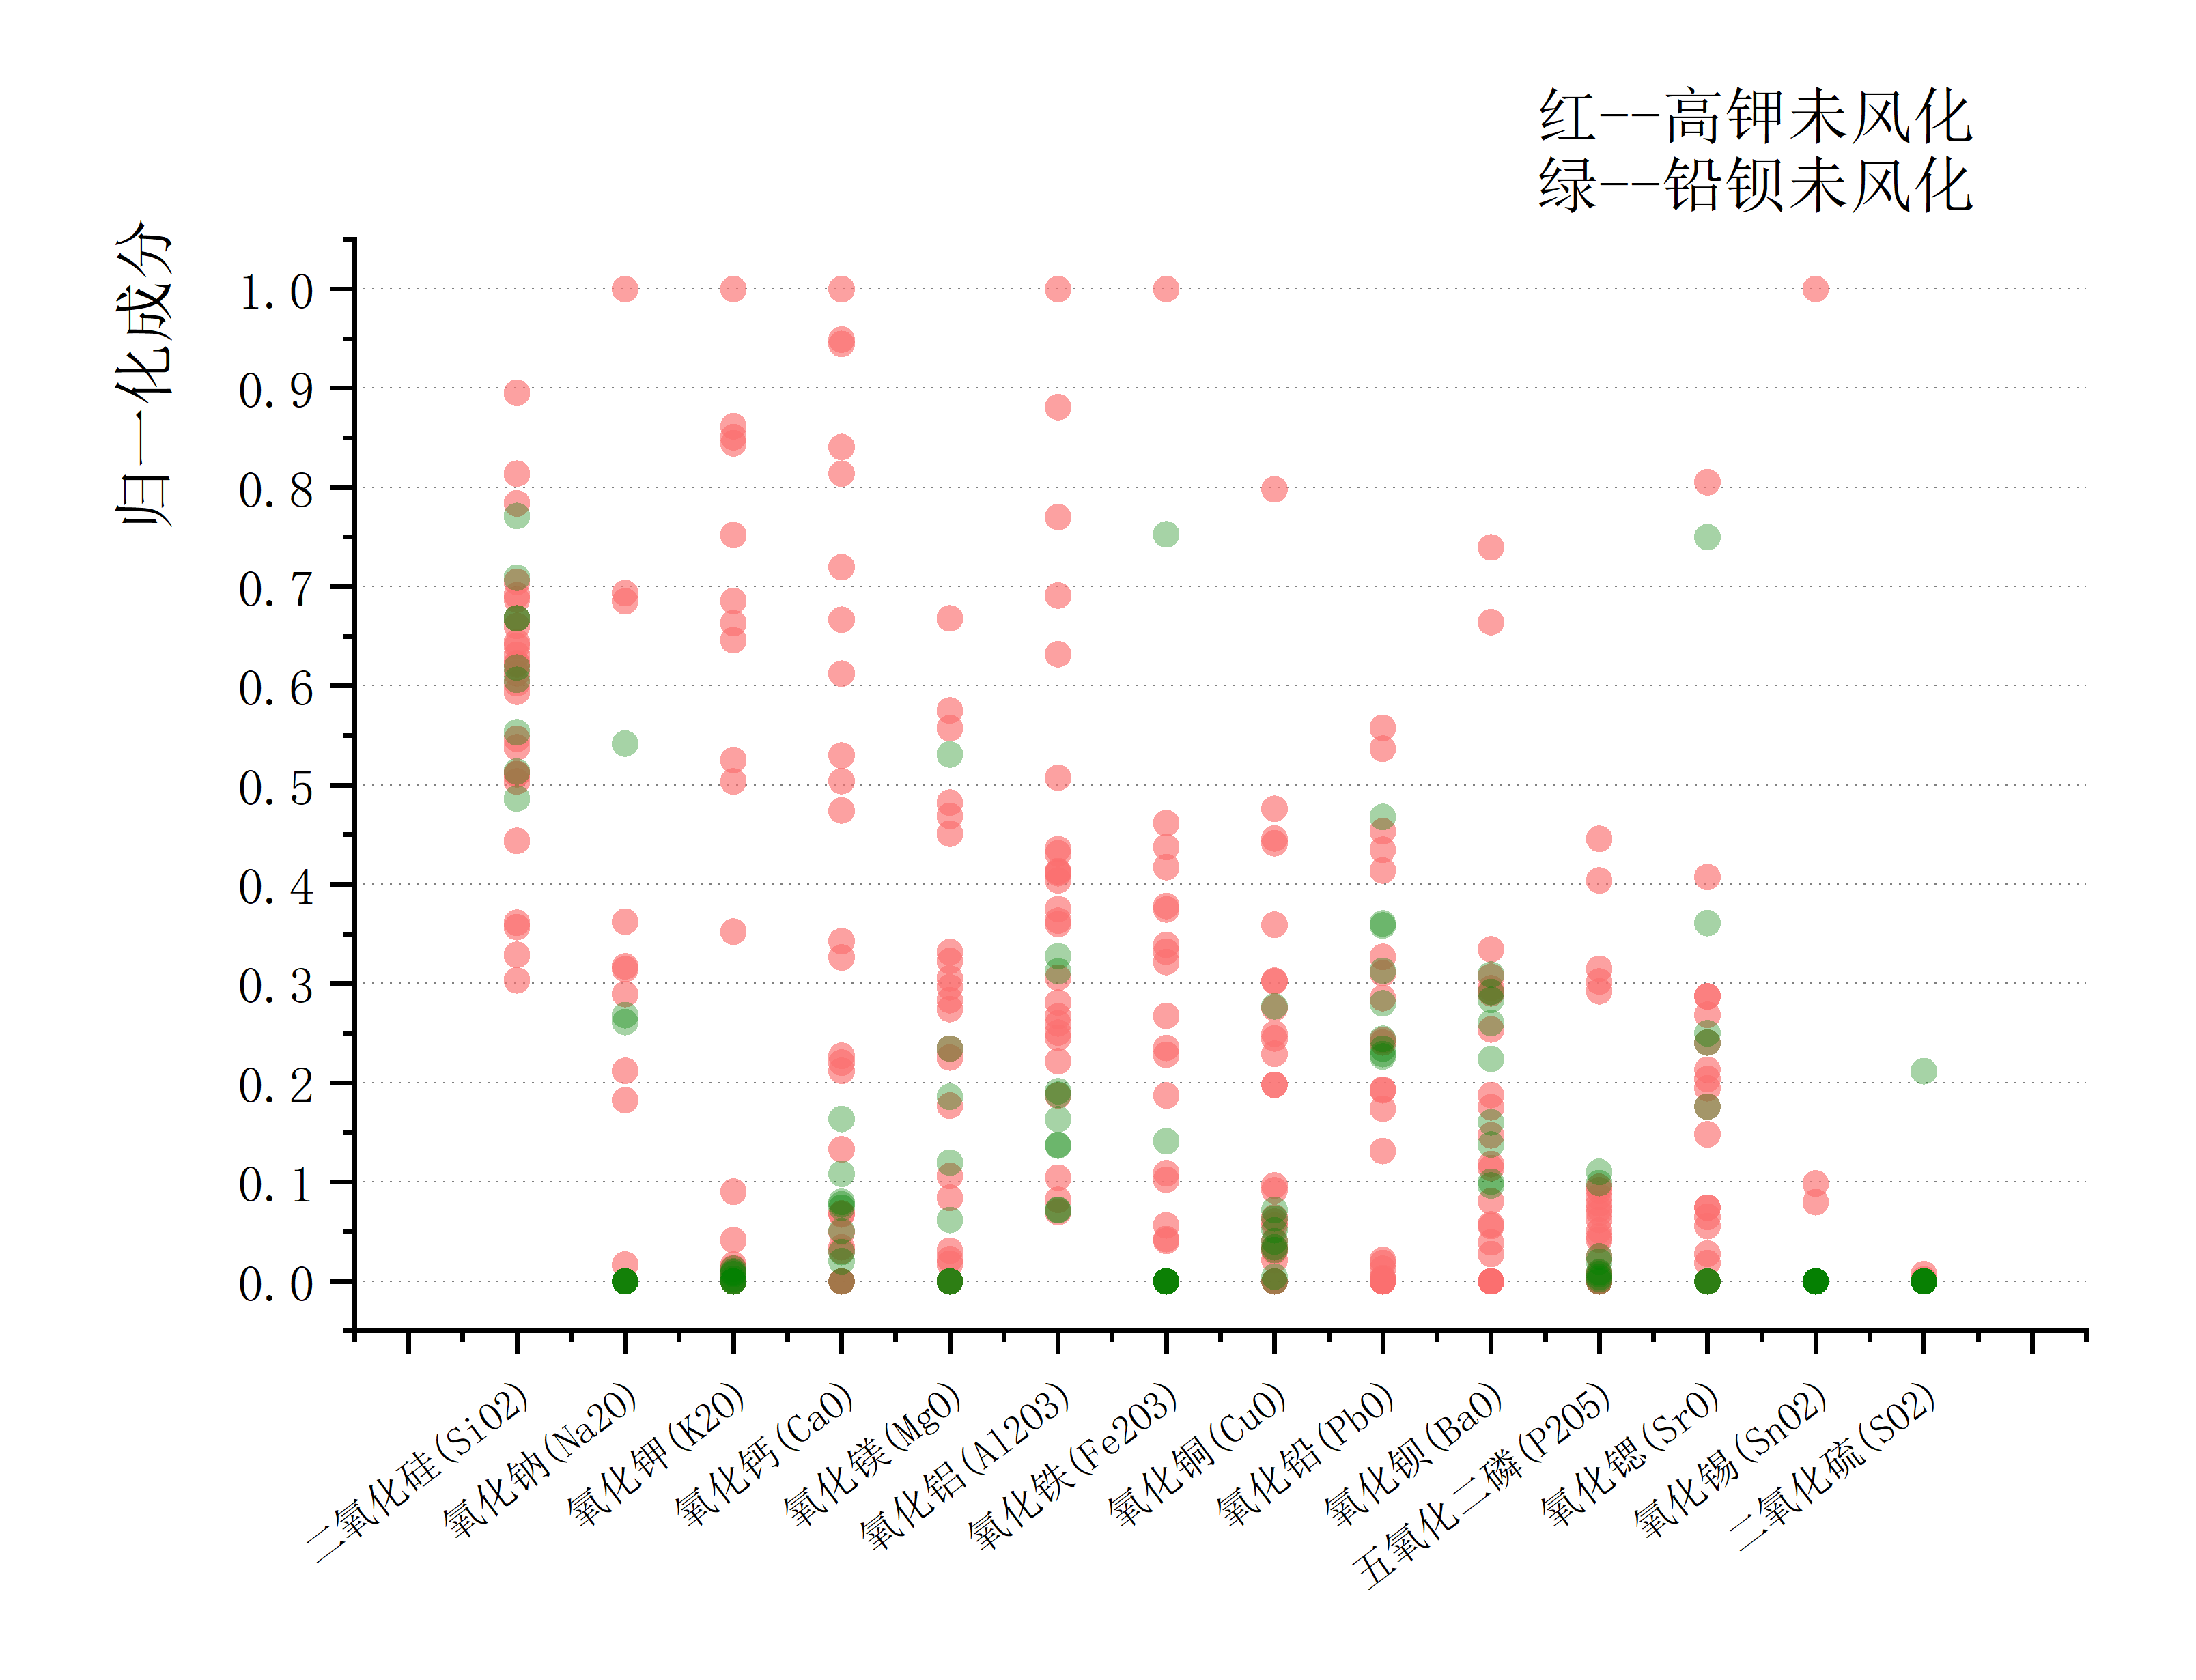
\includegraphics[width=.49\textwidth]{未风化类别分析}
	\caption{风化玻璃(左)与未风化(右)玻璃的类别与成分关系散点图}
	\label{fhgx}
\end{figure}


从风化玻璃的类别与成分关系散点图可以看出:风化后的高钾玻璃的二氧化硅含量明显高于风化后的铅钡玻璃, 且可以看出风化后的高钾玻璃化学成分含量集中在二氧化硅上; 风化后的高钾玻璃不含氧化铅与氧化钡,而风化后的铅钡玻璃的氧化铅和氧化钡的含量很高;


从未风化玻璃的类别与成分关系散点图可以看出:未风化的高钾玻璃在氧化纳、氧化钾和氧化钙含量上明显高于铅钡玻璃且有较明显的分界; 而未风化的高钾玻璃在氧化铅和氧化钡上含量明显低于铅钡玻璃。


\subsubsection{统计规律的定量分析}

在5.1.1节通过散点图进行了定性分析后,本文通过计算类别与各化学成分之间的$spearman$相关系数, 进一步分析玻璃分类的统计规律。


首先,所有玻璃文物的类别与化学成分之间的$spearman$相关系数如表\ref{leihua}所示:

\begin{table}[!h]
	\centering
	\tiny
	\caption{所有玻璃文物的类别与成分的spearman相关系数表}
	\label{leihua}
	\begin{tabular}{|l|l|l|l|l|l|l|l|l|l|l|l|l|l|l|}
		\hline
		\textbf{化学成分}                                                    & \textbf{二氧化硅} & \textbf{氧化纳} & \textbf{氧化钾} & \textbf{氧化钙} & \textbf{氧化镁} & \textbf{氧化铝} & \textbf{氧化铁} & \textbf{氧化铜} & \textbf{氧化铅} & \textbf{氧化钡} & \textbf{五氧化二磷} & \textbf{氧化锶} & \textbf{氧化锡} & \textbf{二氧化硫} \\ \hline
		\textbf{\begin{tabular}[c]{@{}l@{}}Spareman\\ 相关系数\end{tabular}} & -.670**       & 0.117289     & -.583**      & -0.19334     & -0.09478     & -.241*       & -.289*       & -0.22728     & .770**       & .714**       & 0.156965       & .588**       & 0.063272     & -0.06492      \\ \hline
	\end{tabular}
\end{table}

从表中可以看出:在P值为0.01的条件下,玻璃类别与氧化铅、氧化钡有较强的相关性:氧化铅和氧化钡的含量越高, 越有可能是铅钡玻璃;其他相关性并不明显。

接着分别分析风化与否的玻璃类别与化学成分之间的$spearman$相关系数,结果如表\ref{wfhxs}所示:

\begin{table}[!h]
	\centering
	\tiny
	\caption{未风化玻璃文物的类别与成分的spearman相关系数表}
	\label{wfhxs}
	\begin{tabular}{|l|l|l|l|l|l|l|l|l|l|l|l|l|l|l|}
		\hline
		\textbf{化学成分}                                                    & \textbf{二氧化硅} & \textbf{氧化纳} & \textbf{氧化钾} & \textbf{氧化钙} & \textbf{氧化镁} & \textbf{氧化铝} & \textbf{氧化铁} & \textbf{氧化铜} & \textbf{氧化铅} & \textbf{氧化钡} & \textbf{五氧化二磷} & \textbf{氧化锶} & \textbf{氧化锡} & \textbf{二氧化硫} \\ \hline
		\textbf{\begin{tabular}[c]{@{}l@{}}Spareman\\ 相关系数\end{tabular}} & -.442*        & 0.026336     & -.750**      & -.567**      & -.397*       & -.586**      & -0.37817     & -0.38615     & .867**       & .866**       & -0.28823       & .417*        & 0.074139     & -0.22109      \\ \hline
	\end{tabular}
\end{table}

从未风化玻璃文物的类别与成分的spearman相关系数表中可以看出:在P值为0.01的条件下, 玻璃类别与氧化铅、氧化钡和氧化钾有极强的相关性:氧化铅和氧化钡的含量越高, 越有可能是铅钡玻璃; 而氧化钾的含量越高越有可能是高钾玻璃;


从风化玻璃文物的类别与成分的spearman相关系数表中可以看出,在P值为0.01的条件下, 玻璃类别与二氧化硅、氧化钡、氧化铅和氧化锶的含量有着一般的相关性:风化玻璃的二氧化硅含量越高, 越有可能是高钾玻璃类型;氧化钡、氧化铅和氧化锶的含量越高,越有可能是铅钡玻璃类型。


\subsubsection{分类规律总述}

综合玻璃类别与化学成分散点图和$spearman$相关系数的分析可得:高钾玻璃的氧化钾含量明显高于铅钡玻璃; 高钾玻璃的氧化铅和氧化钡含量之和明显低于铅钡玻璃的氧化铅和氧化钡含量之和; 高钾玻璃的二氧化硅含量整体高于铅钡玻璃,但是二者的二氧化硅含量有明显的交集。 基于以上观测,我们推测通过$\frac{P b O+B a O}{K_{2} O}$这一比值可初步确定玻璃文物是高钾玻璃 还是铅钡玻璃。


\section{问题三模型的建立与求解}

观察附件表单三的信息,发现给出的化学成分信息依旧存在空白值,空白含量的大量存在会使得本应是连续 的化学成分信息变得离散,例如:氧化纳、氧化锡、二氧化硫等化学成分由于空白信息过多而变得离散。 决策树是处理这些“离散特征”的好工具, 但除了存在大量空白含量的“离散”化学成分外,表三还提供了如二氧化硅、氧化铝、五氧化二磷等没有空白值的化学 成分,SVM更善于处理这样的化学成分特征,因此本文联合决策树和支持向量机两种分类方法,利用二者特点,训练不同特点的 化学成分信息,得到两个分类模型,最后综合给出最后的类别预测。

\subsection{支持向量机模型的构建}

\subsubsection{支持向量机简介}

支持向量机是经典的线性分类模型,其基本思想是寻找一个合适的超平面将不同类型的样本点分隔开来,特别适用于二分类。 支持向量机采用hinge损失作为自己的损失函数: 

$$L(y \cdot(w \cdot x+b))=[1-y(w \cdot x+b)]{+}$$ 其中$[z]{+}=\left\{\begin{array}{l} z, z>0 \\ 0, z \leq 0 \end{array}\right.$
引入正则化项后,最后的损失函数如下: $$\sum_{i}^{N}\left[1-y_{i}\left(w \cdot x_{i}+b\right)\right]_{+}+\lambda\|w\|^{2}$$

虽然支持向量机是一个线性分类模型,但通过引入适当的核函数,就能实现在高维空间上线性可分从而实现当前空间下非线性分类, 本文便采用的便是使用核技巧的核支持向量机。

\subsubsection{化学成分特征选择}

因为支持向量机是通过寻找一个超平面实现分类的,因此选择良好的化学成分特征尤为重要。根据5.1节的分析可以得出: 氧化钾、氧化铅和氧化钡与化学成分的类别具有较强的相关性,但是考虑到附件表三的氧化钡和氧化铅存在较多未检测到的空白成分, 且整个表单二的数据量极少,为了防止训练时模型过拟合,本文不直接使用氧化铅和氧化钡作为支持向量机模型的输入特征, 而是通过$\frac{PbO+BaO}{k_{2} O}$这一比值的方式将氧化铅和氧化钡引入到模型训练中;同时,考虑到二氧化硅百分比分数 远大于除氧化铅、氧化钡以外的其他化学成分的百分比,因此在训练时避免直接将二氧化硅作为输入,而是通过 $\frac{K_{2}O}{SiO_{2}}$这一比值的方式引入模型训练;最后联合没有空白信息或仅有唯一空白信息的氧化钙、氧化铝 、氧化铁和氧化铜组成最终的输入特征,如表\ref{6-1}所示。

\begin{table}[!h]
	\centering
	\caption{支持向量机输入特征表}
	\label{6-1}
\end{table}

\subsubsection{模型超参数的选择及模型训练}

由于使用的是核支持向量机,使用何种核函数是我们首先要确定的。文章将3种常见的核函数:线性核函数(不使用核函数)、 多项式核函数和高斯核函数均尝试了一遍,最终选择结果最优的核函数。

\begin{figure}[!h]
	\centering
	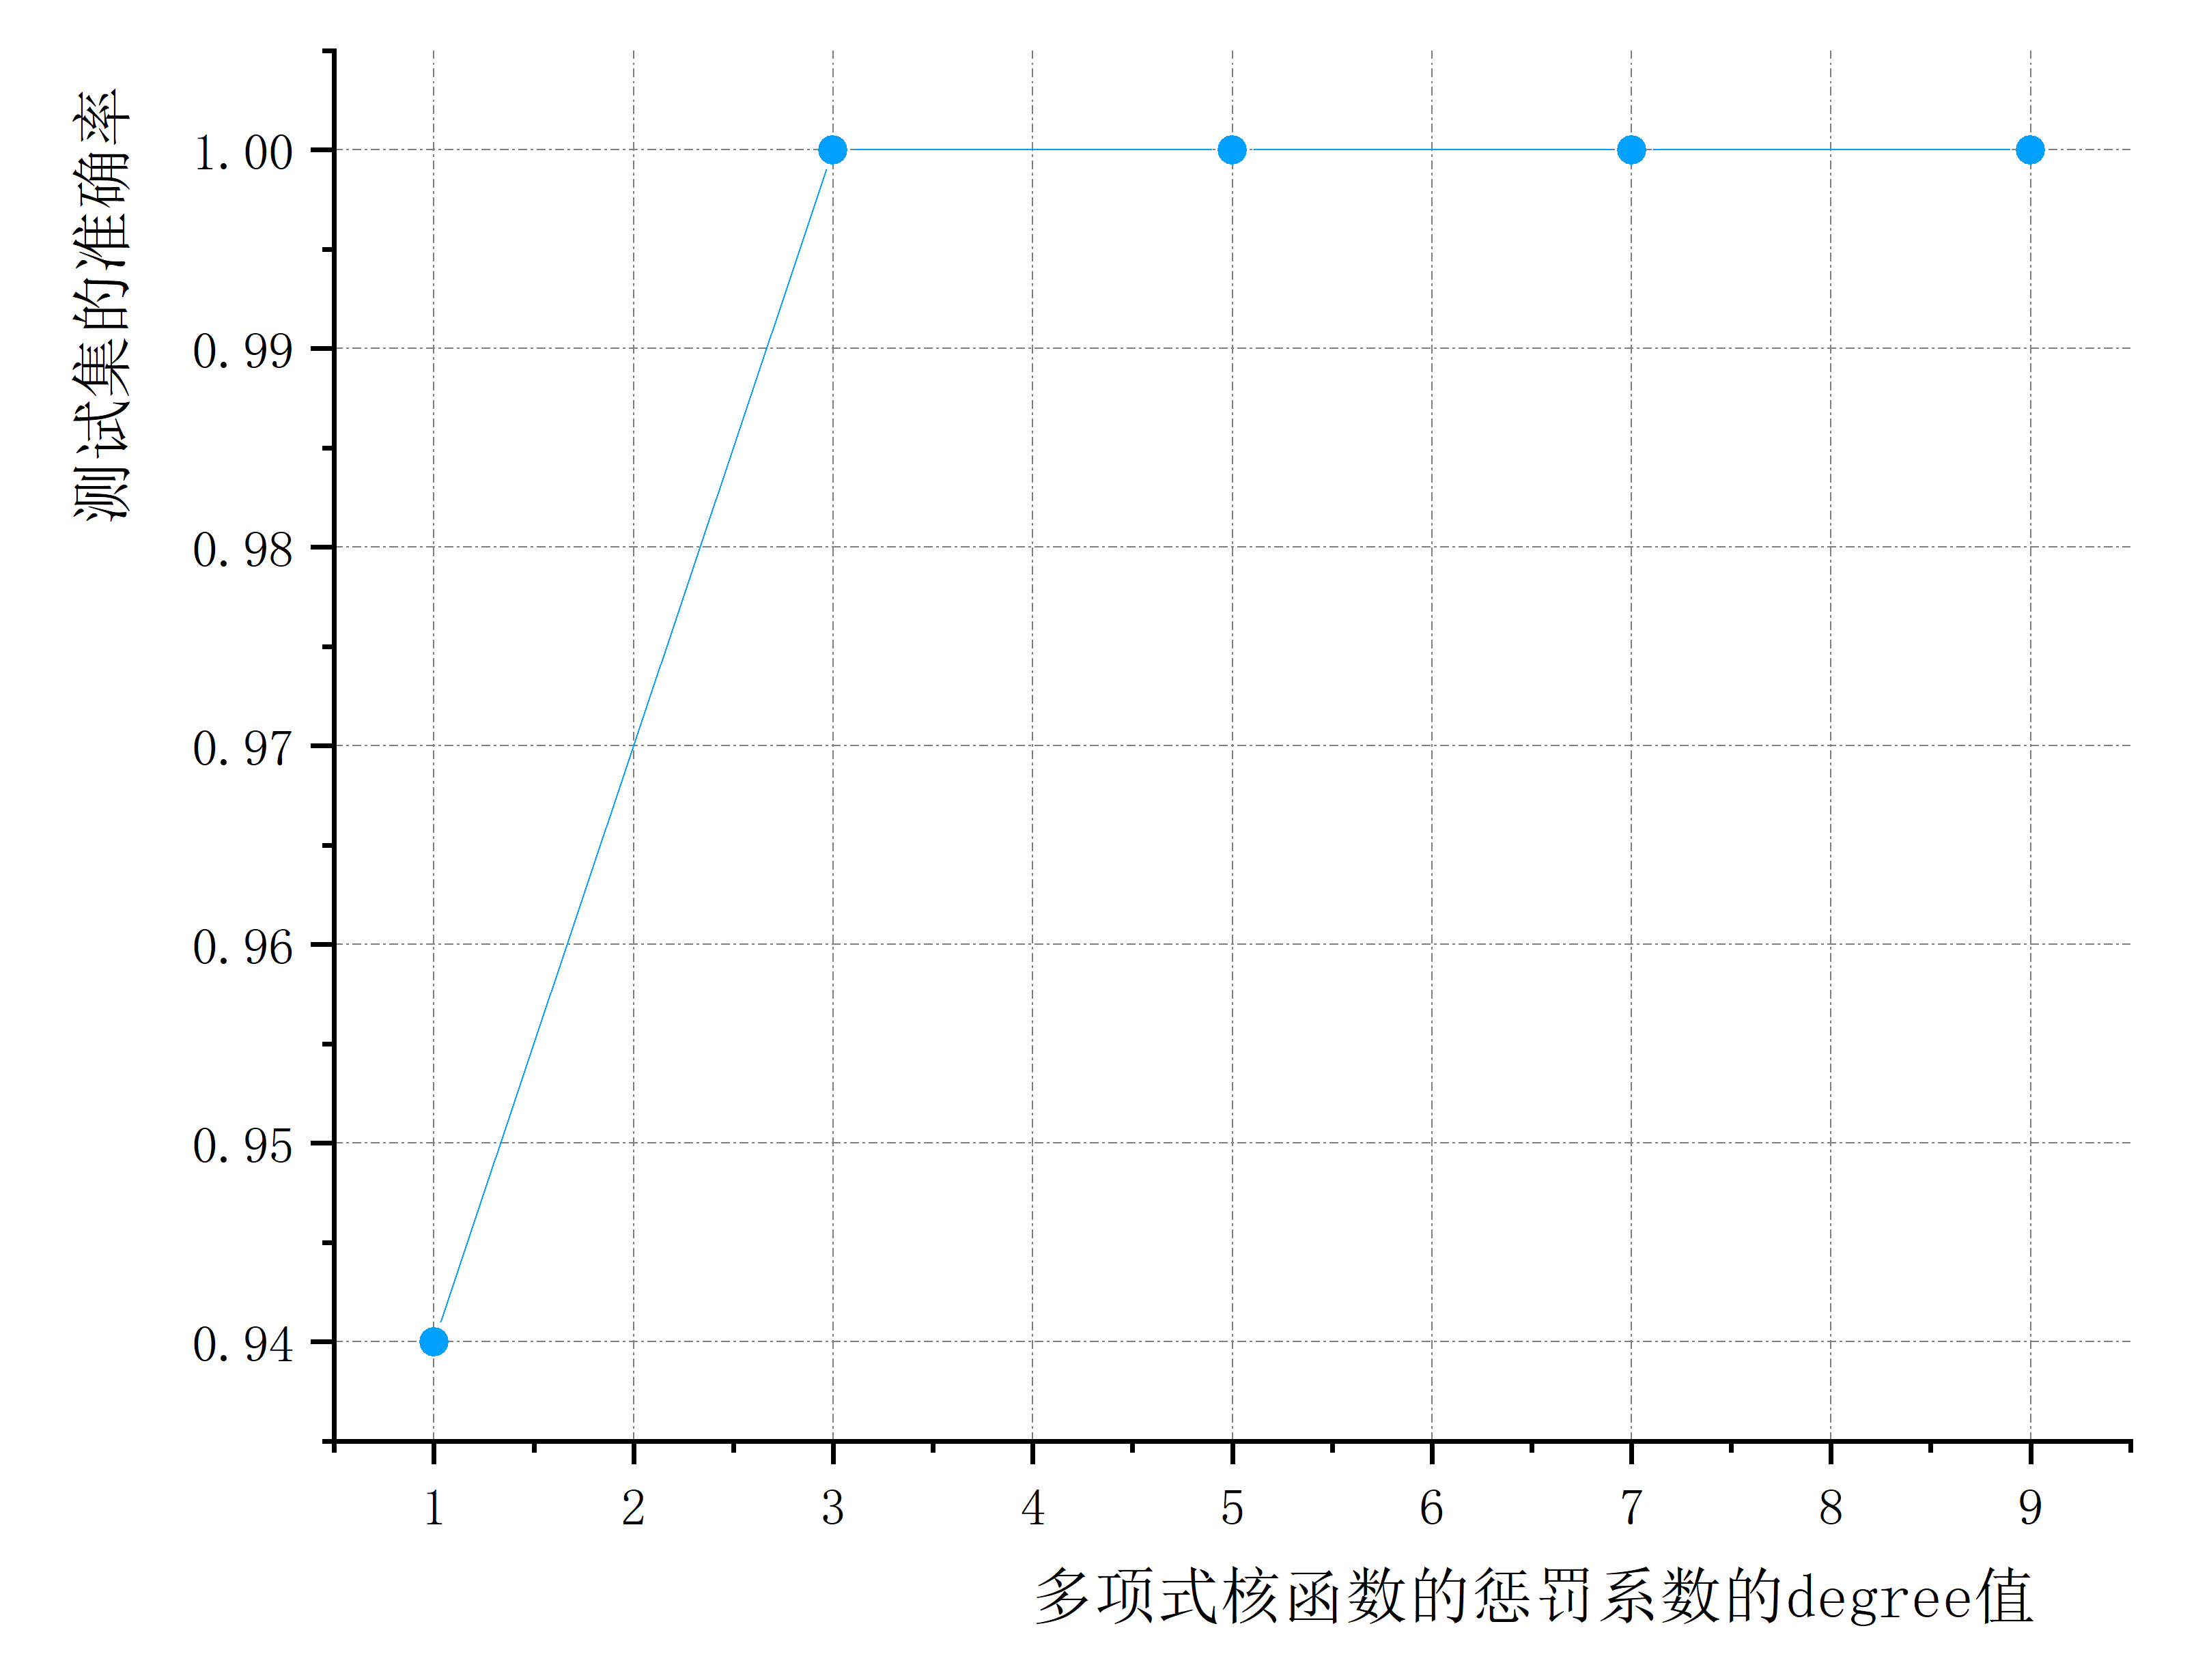
\includegraphics[width=.49\textwidth]{dzql}
	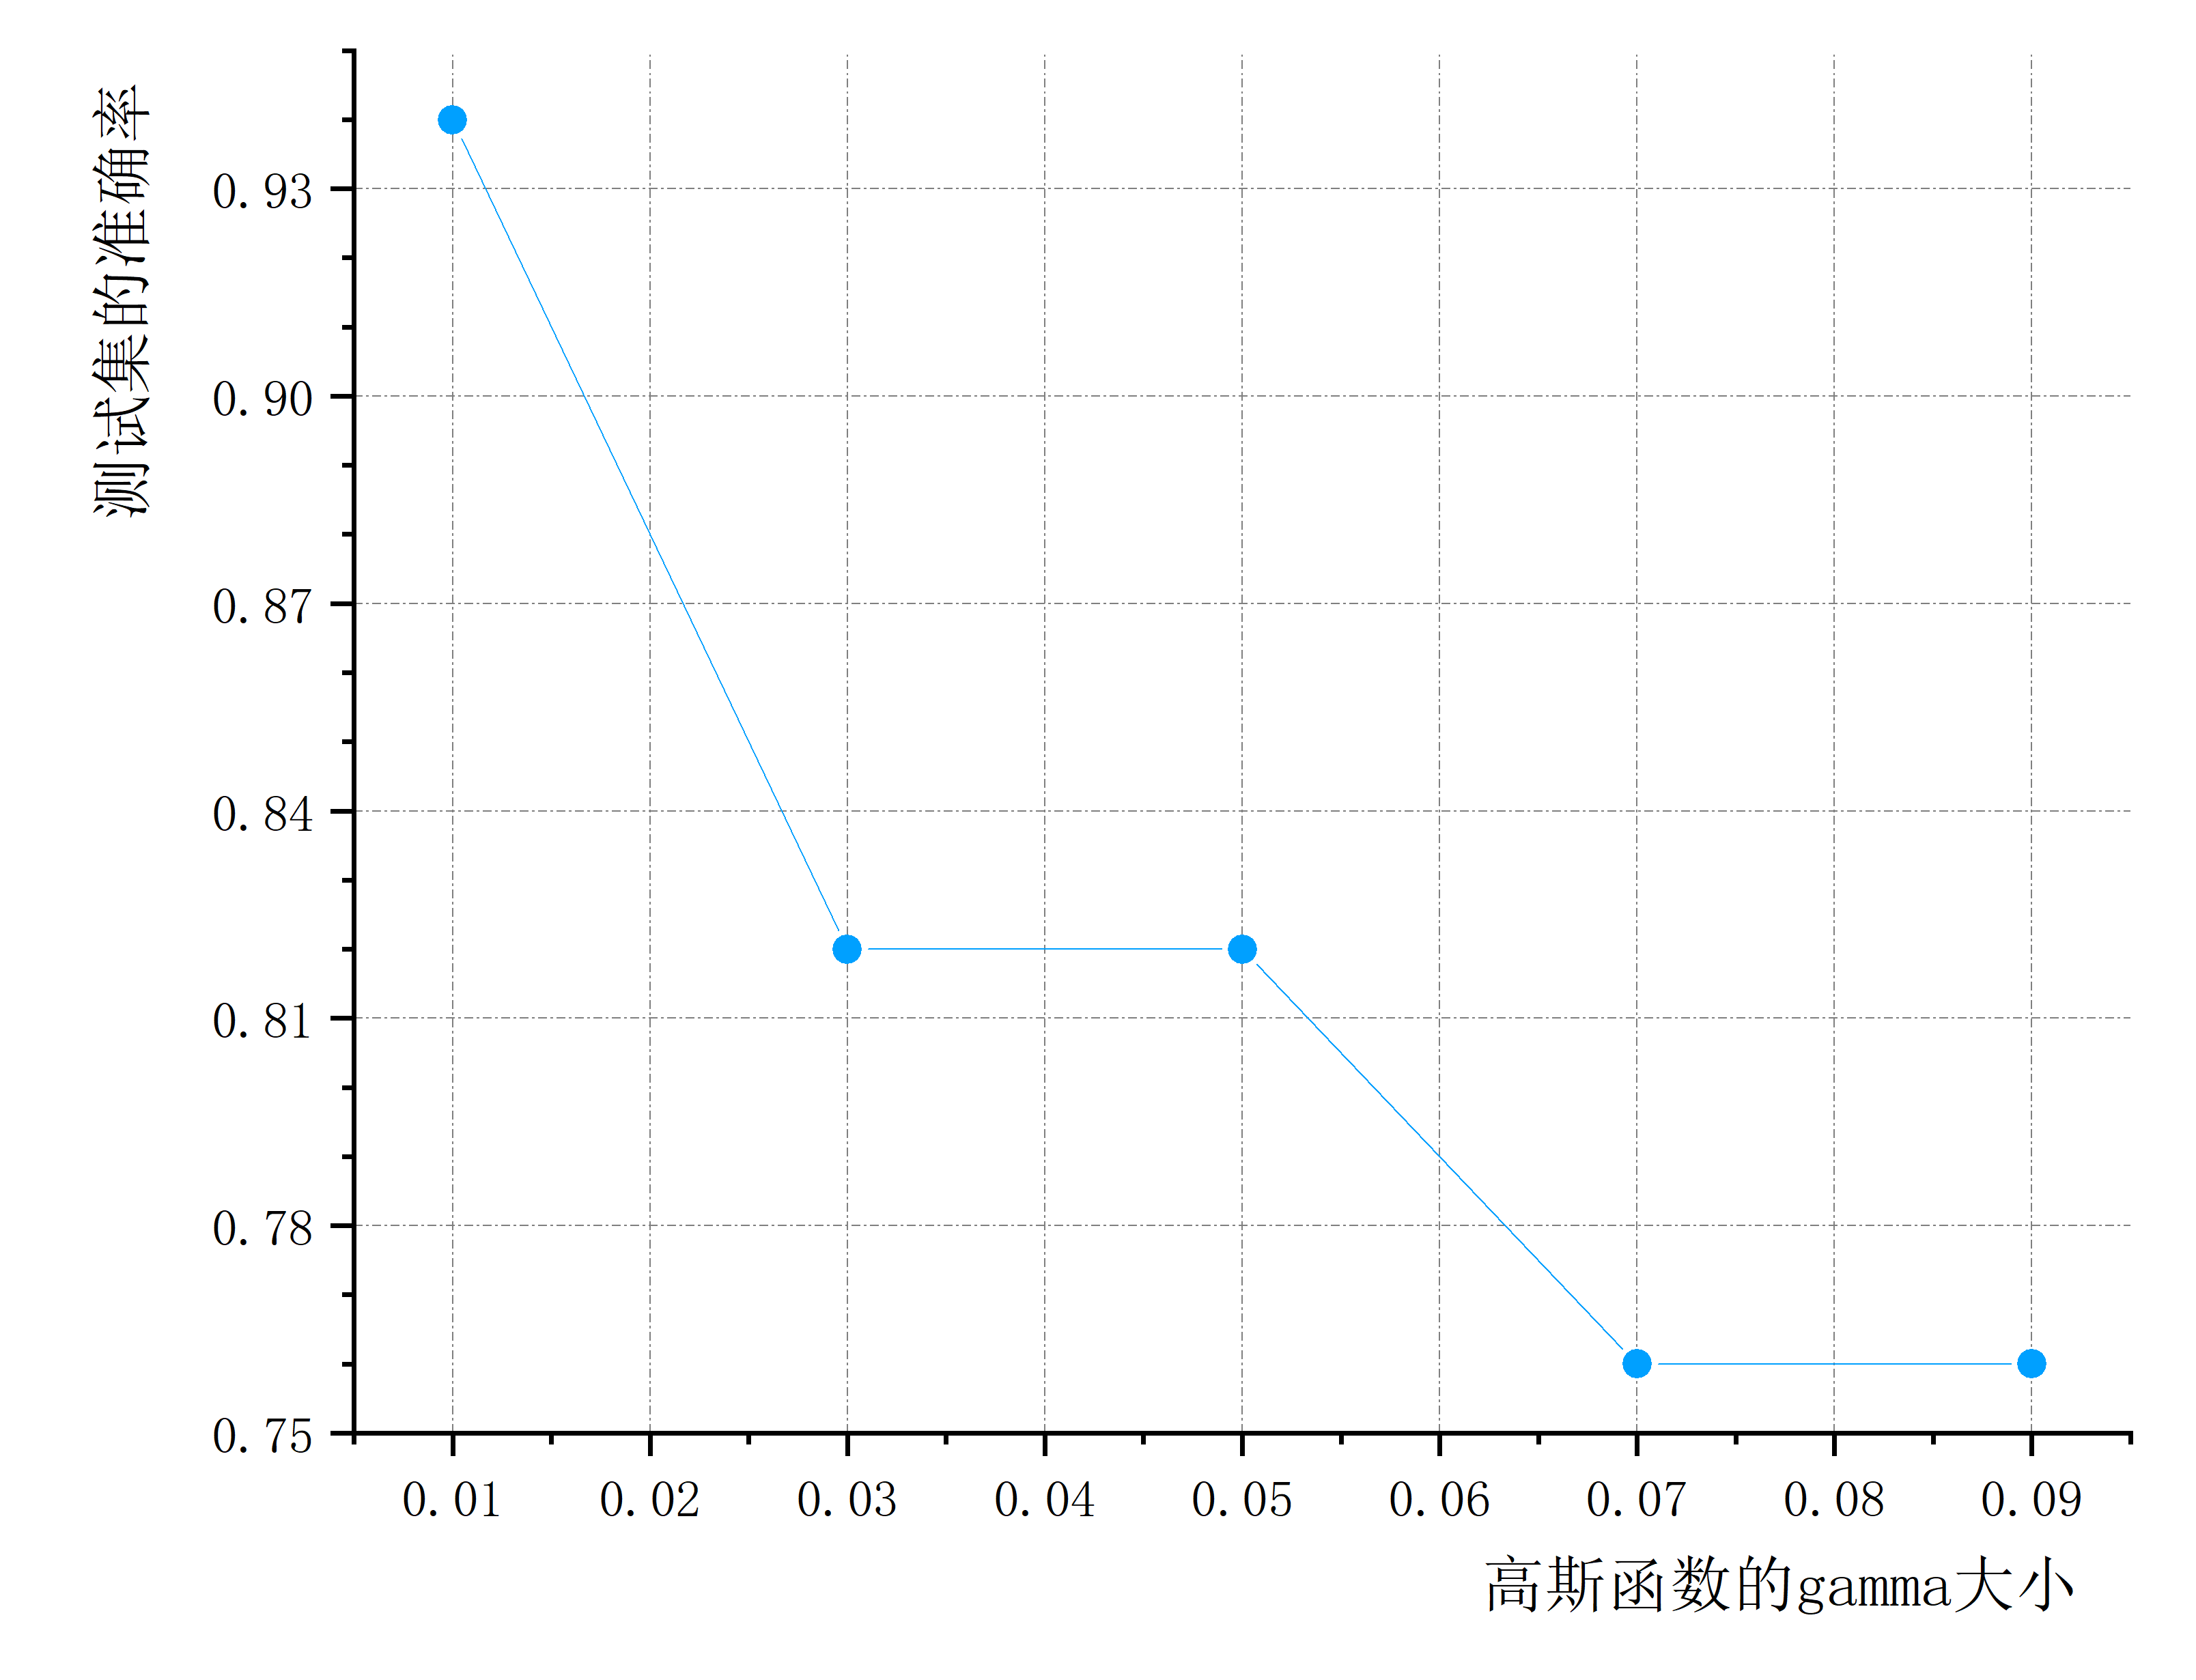
\includegraphics[width=.49\textwidth]{gszql}
	\caption{不同核函数下的测试集的准确度 // *线性核函数默认参数下准确率为94\%,作对照用}
	\label{zqd}
\end{figure}

通过图\ref{zqd}可知,最优的核函数是多项式核函数,且degree选择3。


\subsection{决策树模型的构建}

\subsubsection{CART决策树模型简介}

常见的决策树有许多种,例如:ID3、C4.5、CART分类回归树等等。结合附件中的数据特征:既有连续量又有如是否风化这样的标签量 以及因空白信息过多导致的呈现“标签性质”的连续量,本文最终选择CART分类回归树,一种可以同时处理连续量和标签量的分类算法。 同时,考虑到附件表单二的数据集较小,使用基尼系数相较于使用信息熵能够抑制模型的过拟合。 CART分类回归树采用基尼系数作为衡量一个分割点决策好坏的指标,其数学表达式如下:

 $$\operatorname{Gini}(P)=\sum_{k=1}^{K} P_{k}\left(1-P_{k}\right)=1-\sum_{k=1}^{K} P_{k}^{2}$$
 
其中$K$代表将分类的总类别数,$P_k$是第$k$个类别的概率。 本题是进行二分类,可将表达式进一步化简如下:

 $$\operatorname{Gini}(P)=2 P(1-P)$$
 
在模型训练之前,需要设置一个样本个数阈值和基尼系数阈值作为模型的训练结束条件。通过不断迭代,调整分支使得最后的决策树满足阈值条件 便得到最后的分类模型。

\subsubsection{化学成分特征选取}

数据的输入特征在决策树中充当节点的角色,因此选取合适的输入特征,更能构建一颗优良的决策树。由上文分析可知,高钾玻璃和铅钡玻璃的 二氧化硅、氧化钾、氧化钡和氧化铅含量差异明显,甚至具有肉眼可见的分界面,因此这些属性是良好的决策属性。除此之外:玻璃文物表面 风化与否也是很好的分类特征。观察附件表三所给的数据:二氧化硫、氧化锡和氧化纳这些化学成分由于空白过多,导致其在预测阶段丧失了连续属性, 可以看作标签信号加入进决策树的模型训练中,最终决策树的输入化学成分如表\ref{6-1}所示。

\subsubsection{模型超参数的选择及模型训练}

\subsection{结果预测}

将附件表单三的未知类别的风化信息以及化学成分信息输入多项式核的支持向量机以及决策树得到的对应结果如表\ref{6-2}所示。
\begin{table}[!h]
	\centering
	\caption{决策树输入特征表}
	\label{6-2}
\end{table}


\section{问题4的分析}
\subsection{化学成分关联关系的描述性分析}

对于高钾玻璃,化学成分有如下的关联关系
\begin{itemize}
	\item 在风化进程中$SiO_{2}$含量明显的增多,而$K_{2}O$、$CaO$、$MgO$、$Al_{2}O_{3}$、$Fe_{2}O_{3}$、$CuO$等的含量明显的减小。
	\item 上述几种化学成分的spearman相关系数较高
\end{itemize}


对于铅钡玻璃,化学成分有如下的关联关系
\begin{itemize}
	\item 在风化进程中$SiO_{2}$含量明显的减少,而$PbO$、$Cao$、$BaO$等化学成分含量明显增多,较多的化学成分含量风化前后无明显增多
	\item 铅钡玻璃的化学成分的spearman相关系数较低
\end{itemize}

\subsection{不同玻璃类型间化学成分关系的差异性分析}

本文从化学原理入手,分析不同玻璃类型将化学成分关系的差异性。



\newpage
%参考文献
\begin{thebibliography}{9}%宽度9
	\bibitem[1]{test} 参考文献
\end{thebibliography}




\newpage
%附录
\begin{appendices}
	

\section{高钾玻璃文物样品的$p_{1}$值}
\label{app:gjp1}

\begin{table}[!h]
	\centering
	\small
	\begin{tabular}{@{}cccccccccc@{}}
		\toprule
		\textbf{\begin{tabular}[c]{@{}c@{}}文物\\ 采样点\end{tabular}} & \textbf{类型} & \textbf{\begin{tabular}[c]{@{}c@{}}表面\\ 风化\end{tabular}} & \textbf{\begin{tabular}[c]{@{}c@{}}二氧化硅\\ (SiO2)\end{tabular}} & \textbf{\begin{tabular}[c]{@{}c@{}}氧化钾\\ (K2O)\end{tabular}} & \textbf{\begin{tabular}[c]{@{}c@{}}氧化钙\\ (CaO)\end{tabular}} & \textbf{\begin{tabular}[c]{@{}c@{}}氧化镁\\ (MgO)\end{tabular}} & \textbf{\begin{tabular}[c]{@{}c@{}}氧化铝\\ (Al2O3)\end{tabular}} & \textbf{\begin{tabular}[c]{@{}c@{}}氧化铁\\ (Fe2O3)\end{tabular}} & \textbf{\begin{tabular}[c]{@{}c@{}}高钾的比例\\ (区分风化)\end{tabular}} \\ \midrule
		10                                                        & 高钾          & 风化                                                       & 96.77                                                          & 0.92                                                         & 0.21                                                         & 0.00                                                         & 0.81                                                           & 0.26                                                           & 43.99                                                           \\
		09                                                        & 高钾          & 风化                                                       & 95.02                                                          & 0.59                                                         & 0.62                                                         & 0.00                                                         & 1.32                                                           & 0.32                                                           & 33.34                                                           \\
		07                                                        & 高钾          & 风化                                                       & 92.63                                                          & 0.00                                                         & 1.07                                                         & 0.00                                                         & 1.98                                                           & 0.17                                                           & 28.77                                                           \\
		12                                                        & 高钾          & 风化                                                       & 94.29                                                          & 1.01                                                         & 0.72                                                         & 0.00                                                         & 1.46                                                           & 0.29                                                           & 27.09                                                           \\
		27                                                        & 高钾          & 风化                                                       & 92.72                                                          & 0.00                                                         & 0.94                                                         & 0.54                                                         & 2.51                                                           & 0.20                                                           & 22.13                                                           \\
		22                                                        & 高钾          & 风化                                                       & 92.35                                                          & 0.74                                                         & 1.66                                                         & 0.64                                                         & 3.50                                                           & 0.35                                                           & 13.40                                                           \\
		17                                                        & 高钾          & 无风化                                                      & 60.71                                                          & 5.71                                                         & 0.00                                                         & 0.85                                                         & 0.00                                                           & 1.04                                                           & 7.99                                                            \\
		03部位1                                                     & 高钾          & 无风化                                                      & 87.05                                                          & 5.19                                                         & 2.01                                                         & 0.00                                                         & 4.06                                                           & 0.00                                                           & 7.73                                                            \\
		18                                                        & 高钾          & 无风化                                                      & 79.46                                                          & 9.42                                                         & 0.00                                                         & 1.53                                                         & 3.05                                                           & 0.00                                                           & 5.68                                                            \\
		21                                                        & 高钾          & 无风化                                                      & 76.68                                                          & 0.00                                                         & 4.71                                                         & 1.22                                                         & 6.19                                                           & 2.37                                                           & 5.29                                                            \\
		15                                                        & 高钾          & 无风化                                                      & 61.87                                                          & 7.44                                                         & 0.00                                                         & 1.02                                                         & 3.15                                                           & 1.04                                                           & 4.89                                                            \\
		01                                                        & 高钾          & 无风化                                                      & 69.33                                                          & 9.99                                                         & 6.32                                                         & 0.87                                                         & 3.93                                                           & 1.74                                                           & 3.03                                                            \\
		06部位1                                                     & 高钾          & 无风化                                                      & 67.65                                                          & 7.37                                                         & 0.00                                                         & 1.98                                                         & 11.15                                                          & 2.39                                                           & 2.96                                                            \\
		04                                                        & 高钾          & 无风化                                                      & 65.88                                                          & 9.67                                                         & 7.12                                                         & 1.56                                                         & 6.44                                                           & 2.06                                                           & 2.45                                                            \\
		03部位2                                                     & 高钾          & 无风化                                                      & 61.71                                                          & 12.37                                                        & 5.87                                                         & 1.11                                                         & 5.50                                                           & 2.16                                                           & 2.28                                                            \\
		16                                                        & 高钾          & 无风化                                                      & 65.18                                                          & 14.52                                                        & 8.27                                                         & 0.52                                                         & 6.18                                                           & 0.42                                                           & 2.18                                                            \\
		05                                                        & 高钾          & 无风化                                                      & 61.58                                                          & 10.95                                                        & 7.35                                                         & 1.77                                                         & 7.50                                                           & 2.62                                                           & 2.04                                                            \\
		14                                                        & 高钾          & 无风化                                                      & 62.47                                                          & 12.28                                                        & 8.23                                                         & 0.66                                                         & 9.23                                                           & 0.50                                                           & 2.02                                                            \\
		13                                                        & 高钾          & 无风化                                                      & 59.01                                                          & 12.53                                                        & 8.70                                                         & 0.00                                                         & 6.16                                                           & 2.88                                                           & 1.95                                                            \\
		06部位2                                                     & 高钾          & 无风化                                                      & 59.81                                                          & 7.68                                                         & 5.41                                                         & 1.73                                                         & 10.05                                                          & 6.04                                                           & 1.93                                                            \\ \bottomrule
	\end{tabular}
\end{table}

\newpage

\section{铅钡玻璃文物样品的$p_{2}$值}
\label{app:qbp2}

\begin{table}[!h]
	\centering
	\small
	\begin{tabular}{@{}cccccccc@{}}
		\toprule
		\textbf{\begin{tabular}[c]{@{}c@{}}文物\\ 采样点\end{tabular}} & \textbf{类型} & \textbf{\begin{tabular}[c]{@{}c@{}}表面\\ 风化\end{tabular}} & \textbf{\begin{tabular}[c]{@{}c@{}}二氧化硅\\ (SiO2)\end{tabular}} & \textbf{\begin{tabular}[c]{@{}c@{}}氧化铜\\ (CuO)\end{tabular}} & \textbf{\begin{tabular}[c]{@{}c@{}}氧化铅\\ (PbO)\end{tabular}} & \textbf{\begin{tabular}[c]{@{}c@{}}氧化钡\\ (BaO)\end{tabular}} & \textbf{\begin{tabular}[c]{@{}c@{}}铅钡的比例\\ (区分风化)\end{tabular}} \\ \midrule
		26严重风化点                                                   & 铅钡          & 风化                                                       & 3.72                                                           & 3.60                                                         & 29.92                                                        & 35.45                                                        & 0.05                                                            \\
		08严重风化点                                                   & 铅钡          & 风化                                                       & 4.61                                                           & 3.14                                                         & 32.45                                                        & 30.62                                                        & 0.07                                                            \\
		43部位1                                                     & 铅钡          & 风化                                                       & 12.41                                                          & 5.35                                                         & 59.85                                                        & 7.29                                                         & 0.17                                                            \\
		40                                                        & 铅钡          & 风化                                                       & 16.71                                                          & 0.00                                                         & 70.21                                                        & 6.69                                                         & 0.22                                                            \\
		54严重风化点                                                   & 铅钡          & 风化                                                       & 17.11                                                          & 1.34                                                         & 58.46                                                        & 0.00                                                         & 0.29                                                            \\
		54                                                        & 铅钡          & 风化                                                       & 22.28                                                          & 0.83                                                         & 55.46                                                        & 7.04                                                         & 0.35                                                            \\
		50                                                        & 铅钡          & 风化                                                       & 17.98                                                          & 1.13                                                         & 44.00                                                        & 14.20                                                        & 0.30                                                            \\
		51部位2                                                     & 铅钡          & 风化                                                       & 21.35                                                          & 0.75                                                         & 51.34                                                        & 0.00                                                         & 0.41                                                            \\
		41                                                        & 铅钡          & 风化                                                       & 18.46                                                          & 0.19                                                         & 44.12                                                        & 9.76                                                         & 0.34                                                            \\
		39                                                        & 铅钡          & 风化                                                       & 26.25                                                          & 0.88                                                         & 61.03                                                        & 7.22                                                         & 0.38                                                            \\
		43部位2                                                     & 铅钡          & 风化                                                       & 21.70                                                          & 1.51                                                         & 44.75                                                        & 3.26                                                         & 0.44                                                            \\
		52                                                        & 铅钡          & 风化                                                       & 25.74                                                          & 0.70                                                         & 47.42                                                        & 8.64                                                         & 0.45                                                            \\
		57                                                        & 铅钡          & 风化                                                       & 25.42                                                          & 1.16                                                         & 45.10                                                        & 17.30                                                        & 0.40                                                            \\
		51部位1                                                     & 铅钡          & 风化                                                       & 24.61                                                          & 1.37                                                         & 40.24                                                        & 8.94                                                         & 0.49                                                            \\
		38                                                        & 铅钡          & 风化                                                       & 32.93                                                          & 0.73                                                         & 49.31                                                        & 9.79                                                         & 0.55                                                            \\
		26                                                        & 铅钡          & 风化                                                       & 19.79                                                          & 10.57                                                        & 29.53                                                        & 32.25                                                        & 0.27                                                            \\
		19                                                        & 铅钡          & 风化                                                       & 29.64                                                          & 3.51                                                         & 42.82                                                        & 5.35                                                         & 0.57                                                            \\
		08                                                        & 铅钡          & 风化                                                       & 20.14                                                          & 10.41                                                        & 28.68                                                        & 31.23                                                        & 0.29                                                            \\
		56                                                        & 铅钡          & 风化                                                       & 29.15                                                          & 0.79                                                         & 41.25                                                        & 15.45                                                        & 0.51                                                            \\
		02                                                        & 铅钡          & 风化                                                       & 36.28                                                          & 0.26                                                         & 47.43                                                        & 0.00                                                         & 0.76                                                            \\
		34                                                        & 铅钡          & 风化                                                       & 35.78                                                          & 1.51                                                         & 46.55                                                        & 10.00                                                        & 0.62                                                            \\
		58                                                        & 铅钡          & 风化                                                       & 30.39                                                          & 3.13                                                         & 39.35                                                        & 7.66                                                         & 0.61                                                            \\
		49                                                        & 铅钡          & 风化                                                       & 28.79                                                          & 0.70                                                         & 34.18                                                        & 6.10                                                         & 0.70                                                            \\
		30部位1                                                     & 铅钡          & 无风化                                                      & 34.34                                                          & 0.00                                                         & 39.22                                                        & 10.29                                                        & 0.69                                                            \\
		36                                                        & 铅钡          & 风化                                                       & 39.57                                                          & 0.68                                                         & 41.61                                                        & 10.83                                                        & 0.74                                                            \\
		30部位2                                                     & 铅钡          & 无风化                                                      & 36.93                                                          & 0.00                                                         & 37.74                                                        & 10.35                                                        & 0.77                                                            \\
		24                                                        & 铅钡          & 无风化                                                      & 31.94                                                          & 8.46                                                         & 29.14                                                        & 26.23                                                        & 0.50                                                            \\
		11                                                        & 铅钡          & 风化                                                       & 33.59                                                          & 4.93                                                         & 25.39                                                        & 14.61                                                        & 0.75                                                            \\
		50未风化点                                                    & 铅钡          & \begin{tabular}[c]{@{}c@{}}风化\\ (实际无风化)\end{tabular}     & 45.02                                                          & 0.70                                                         & 30.61                                                        & 6.22                                                         & 1.20                                                            \\
		55                                                        & 铅钡          & 无风化                                                      & 49.01                                                          & 0.86                                                         & 32.92                                                        & 7.95                                                         & 1.17                                                            \\
		25未风化点                                                    & 铅钡          & \begin{tabular}[c]{@{}c@{}}风化\\ (实际无风化)\end{tabular}     & 50.61                                                          & 1.12                                                         & 31.90                                                        & 6.65                                                         & 1.28                                                            \\
		47                                                        & 铅钡          & 无风化                                                      & 51.54                                                          & 0.65                                                         & 25.40                                                        & 9.23                                                         & 1.46                                                            \\
		46                                                        & 铅钡          & 无风化                                                      & 55.21                                                          & 0.77                                                         & 25.25                                                        & 10.06                                                        & 1.53                                                            \\
		42未风化点1                                                   & 铅钡          & \begin{tabular}[c]{@{}c@{}}风化\\ (实际无风化)\end{tabular}     & 51.26                                                          & 2.67                                                         & 21.88                                                        & 10.47                                                        & 1.46                                                            \\
				\bottomrule
	\end{tabular}
\end{table}
\begin{table}[!h]
\centering
\small
\begin{tabular}{@{}cccccccc@{}}
\toprule
\textbf{\begin{tabular}[c]{@{}c@{}}文物\\ 采样点\end{tabular}} & \textbf{类型} & \textbf{\begin{tabular}[c]{@{}c@{}}表面\\ 风化\end{tabular}} & \textbf{\begin{tabular}[c]{@{}c@{}}二氧化硅\\ (SiO2)\end{tabular}} & \textbf{\begin{tabular}[c]{@{}c@{}}氧化铜\\ (CuO)\end{tabular}} & \textbf{\begin{tabular}[c]{@{}c@{}}氧化铅\\ (PbO)\end{tabular}} & \textbf{\begin{tabular}[c]{@{}c@{}}氧化钡\\ (BaO)\end{tabular}} & \textbf{\begin{tabular}[c]{@{}c@{}}铅钡的比例\\ (区分风化)\end{tabular}} \\ \midrule
		49未风化点                                                    & 铅钡          & \begin{tabular}[c]{@{}c@{}}风化\\ (实际无风化)\end{tabular}     & 54.61                                                          & 0.45                                                         & 23.02                                                        & 4.19                                                         & 1.97                                                            \\
		42未风化点2                                                   & 铅钡          & \begin{tabular}[c]{@{}c@{}}风化\\ (实际无风化)\end{tabular}     & 51.33                                                          & 2.72                                                         & 20.12                                                        & 10.88                                                        & 1.52                                                            \\
		35                                                        & 铅钡          & 无风化                                                      & 65.91                                                          & 0.16                                                         & 22.05                                                        & 5.68                                                         & 2.36                                                            \\
		23未风化点                                                    & 铅钡          & \begin{tabular}[c]{@{}c@{}}风化\\ (实际无风化)\end{tabular}     & 53.79                                                          & 2.99                                                         & 16.98                                                        & 11.86                                                        & 1.69                                                            \\
		48                                                        & 铅钡          & 风化                                                       & 53.33                                                          & 0.00                                                         & 15.71                                                        & 7.31                                                         & 2.32                                                            \\
		37                                                        & 铅钡          & 无风化                                                      & 60.12                                                          & 3.01                                                         & 17.24                                                        & 10.34                                                        & 1.97                                                            \\
		32                                                        & 铅钡          & 无风化                                                      & 69.71                                                          & 0.11                                                         & 19.76                                                        & 4.88                                                         & 2.82                                                            \\
		45                                                        & 铅钡          & 无风化                                                      & 61.28                                                          & 0.53                                                         & 15.99                                                        & 10.96                                                        & 2.23                                                            \\
		28未风化点                                                    & 铅钡          & \begin{tabular}[c]{@{}c@{}}风化\\ (实际无风化)\end{tabular}     & 68.08                                                          & 0.33                                                         & 17.14                                                        & 4.04                                                         & 3.17                                                            \\
		31                                                        & 铅钡          & 无风化                                                      & 65.91                                                          & 0.44                                                         & 16.55                                                        & 3.42                                                         & 3.23                                                            \\
		20                                                        & 铅钡          & 无风化                                                      & 37.36                                                          & 4.78                                                         & 9.30                                                         & 23.55                                                        & 0.99                                                            \\
		44未风化点                                                    & 铅钡          & \begin{tabular}[c]{@{}c@{}}风化\\ (实际无风化)\end{tabular}     & 60.74                                                          & 0.43                                                         & 13.61                                                        & 5.22                                                         & 3.15                                                            \\
		53未风化点                                                    & 铅钡          & \begin{tabular}[c]{@{}c@{}}风化\\ (实际无风化)\end{tabular}     & 63.66                                                          & 0.54                                                         & 13.66                                                        & 8.99                                                         & 2.75                                                            \\
		33                                                        & 铅钡          & 无风化                                                      & 75.51                                                          & 0.47                                                         & 16.16                                                        & 3.55                                                         & 3.74                                                            \\
		29未风化点                                                    & 铅钡          & 无风化                                                      & 63.30                                                          & 0.74                                                         & 12.31                                                        & 2.03                                                         & 4.20                                                            \\ \bottomrule
	\end{tabular}
\end{table}


\newpage
$ $
\newpage

\section{风化后高钾玻璃化学成分的预测}
\label{app:yucel}

\begin{table}[!h]
	\centering
	\tiny
		\begin{tabular}{@{}ccccccccccccccc@{}}
			\toprule
			\textbf{\begin{tabular}[c]{@{}c@{}}文物\\ 采样点\end{tabular}} & \textbf{\begin{tabular}[c]{@{}c@{}}二氧化硅\\ (SiO2)\end{tabular}} & \textbf{\begin{tabular}[c]{@{}c@{}}氧化钠\\ (Na2O)\end{tabular}} & \textbf{\begin{tabular}[c]{@{}c@{}}氧化钾\\ (K2O)\end{tabular}} & \textbf{\begin{tabular}[c]{@{}c@{}}氧化钙\\ (CaO)\end{tabular}} & \textbf{\begin{tabular}[c]{@{}c@{}}氧化镁\\ (MgO)\end{tabular}} & \textbf{\begin{tabular}[c]{@{}c@{}}氧化铝\\ (Al2O3)\end{tabular}} & \textbf{\begin{tabular}[c]{@{}c@{}}氧化铁\\ (Fe2O3)\end{tabular}} & \textbf{\begin{tabular}[c]{@{}c@{}}氧化铜\\ (CuO)\end{tabular}} & \textbf{\begin{tabular}[c]{@{}c@{}}氧化铅\\ (PbO)\end{tabular}} & \textbf{\begin{tabular}[c]{@{}c@{}}氧化钡\\ (BaO)\end{tabular}} & \textbf{\begin{tabular}[c]{@{}c@{}}五氧化二磷\\ (P2O5)\end{tabular}} & \textbf{\begin{tabular}[c]{@{}c@{}}氧化锶\\ (SrO)\end{tabular}} & \textbf{\begin{tabular}[c]{@{}c@{}}氧化锡\\ (SnO2)\end{tabular}} & \textbf{\begin{tabular}[c]{@{}c@{}}二氧化硫\\ (SO2)\end{tabular}} \\ \midrule
			\textbf{12}                                               & 67.549                                                         & 0.976                                                         & 9.951                                                        & 4.472                                                        & 0.862                                                        & 5.431                                                          & 1.830                                                          & 2.360                                                        & 0.380                                                        & 0.513                                                        & 0.150                                                           & 0.036                                                        & 0.169                                                         & 0.087                                                         \\
			\textbf{22}                                               & 71.648                                                         & 0.976                                                         & 9.312                                                        & 5.361                                                        & 1.523                                                        & 7.470                                                          & 1.889                                                          & 1.236                                                        & 0.380                                                        & 0.513                                                        & 0.210                                                           & 0.036                                                        & 0.169                                                         & 0.087                                                         \\
			\textbf{9}                                                & 72.596                                                         & 0.976                                                         & 8.994                                                        & 4.321                                                        & 0.868                                                        & 5.289                                                          & 1.862                                                          & 2.267                                                        & 0.380                                                        & 0.513                                                        & 0.350                                                           & 0.036                                                        & 0.169                                                         & 0.087                                                         \\
			\textbf{27}                                               & 70.284                                                         & 0.976                                                         & 8.373                                                        & 4.657                                                        & 0.540                                                        & 2.510                                                          & 1.740                                                          & 2.254                                                        & 0.380                                                        & 0.513                                                        & 0.360                                                           & 0.036                                                        & 0.169                                                         & 0.087                                                         \\
			\textbf{7}                                                & 70.183                                                         & 0.976                                                         & 8.394                                                        & 4.783                                                        & 0.864                                                        & 5.947                                                          & 1.709                                                          & 3.954                                                        & 0.380                                                        & 0.513                                                        & 0.610                                                           & 0.036                                                        & 0.169                                                         & 0.087                                                         \\
			\textbf{10}                                               & 75.371                                                         & 0.976                                                         & 9.343                                                        & 3.912                                                        & 0.862                                                        & 4.779                                                          & 1.800                                                          & 1.550                                                        & 0.380                                                        & 0.513                                                        & 0.000                                                           & 0.036                                                        & 0.169                                                         & 0.087                                                         \\ \bottomrule
		\end{tabular}
	\end{table}

\section{风化后铅钡玻璃化学成分的预测}
\label{app:qbycl}

\begin{table}[!h]
	\centering
	\tiny 
		\begin{tabular}{@{}ccccccccccccccc@{}}
			\toprule
			\textbf{文物采样点}   & \textbf{\begin{tabular}[c]{@{}c@{}}二氧化硅\\ (SiO2)\end{tabular}} & \textbf{\begin{tabular}[c]{@{}c@{}}氧化钠\\ (Na2O)\end{tabular}} & \textbf{\begin{tabular}[c]{@{}c@{}}氧化钾\\ (K2O)\end{tabular}} & \textbf{\begin{tabular}[c]{@{}c@{}}氧化钙\\ (CaO)\end{tabular}} & \textbf{\begin{tabular}[c]{@{}c@{}}氧化镁\\ (MgO)\end{tabular}} & \textbf{\begin{tabular}[c]{@{}c@{}}氧化铝\\ (Al2O3)\end{tabular}} & \textbf{\begin{tabular}[c]{@{}c@{}}氧化铁\\ (Fe2O3)\end{tabular}} & \textbf{\begin{tabular}[c]{@{}c@{}}氧化铜\\ (CuO)\end{tabular}} & \textbf{\begin{tabular}[c]{@{}c@{}}氧化铅\\ (PbO)\end{tabular}} & \textbf{\begin{tabular}[c]{@{}c@{}}氧化钡\\ (BaO)\end{tabular}} & \textbf{\begin{tabular}[c]{@{}c@{}}五氧化二磷\\ (P2O5)\end{tabular}} & \textbf{\begin{tabular}[c]{@{}c@{}}氧化锶\\ (SrO)\end{tabular}} & \textbf{\begin{tabular}[c]{@{}c@{}}氧化锡\\ (SnO2)\end{tabular}} & \textbf{\begin{tabular}[c]{@{}c@{}}二氧化硫\\ (SO2)\end{tabular}} \\ \midrule
			\textbf{48}      & 75.17                                                          & 2.31                                                          & 0.42                                                         & 1.47                                                         & 1.58                                                         & 15.38                                                          & 1.23                                                           & -0.86                                                        & -5.61                                                        & 4.54                                                         & -3.27                                                           & 0.10                                                         & 1.31                                                          & 0.00                                                          \\
			\textbf{02}      & 66.20                                                          & 1.50                                                          & 1.16                                                         & 0.97                                                         & 1.20                                                         & 7.45                                                           & 2.02                                                           & -0.59                                                        & 26.62                                                        & -2.86                                                        & -0.67                                                           & 0.04                                                         & -0.02                                                         & 0.00                                                          \\
			\textbf{11}      & 66.29                                                          & 1.47                                                          & 0.31                                                         & 2.17                                                         & 0.71                                                         & 4.33                                                           & 0.15                                                           & 4.22                                                         & 4.21                                                         & 11.90                                                        & 5.21                                                            & 0.22                                                         & -0.02                                                         & 0.00                                                          \\
			\textbf{36}      & 71.84                                                          & 3.72                                                          & 0.23                                                         & -1.01                                                        & -0.01                                                        & 3.18                                                           & 0.48                                                           & -0.17                                                        & 20.64                                                        & 8.33                                                         & -4.32                                                           & 0.07                                                         & -0.02                                                         & 0.00                                                          \\
			\textbf{49}      & 60.70                                                          & 1.52                                                          & 0.09                                                         & 3.29                                                         & 1.52                                                         & 7.12                                                           & 2.97                                                           & -0.15                                                        & 13.53                                                        & 3.44                                                         & 7.13                                                            & 0.32                                                         & -0.02                                                         & 0.00                                                          \\
			\textbf{34}      & 65.73                                                          & 1.49                                                          & 0.35                                                         & -0.62                                                        & -0.01                                                        & 3.14                                                           & 0.62                                                           & 0.69                                                         & 26.21                                                        & 7.32                                                         & -4.03                                                           & 0.07                                                         & -0.02                                                         & 0.00                                                          \\
			\textbf{58}      & 62.72                                                          & 1.53                                                          & 0.44                                                         & 2.18                                                         & 0.80                                                         & 5.19                                                           & 1.03                                                           & 2.29                                                         & 18.62                                                        & 5.02                                                         & 4.94                                                            & 0.09                                                         & -0.02                                                         & 0.00                                                          \\
			\textbf{19}      & 62.16                                                          & 1.48                                                          & 0.09                                                         & 1.56                                                         & 0.60                                                         & 5.30                                                           & 1.49                                                           & 2.71                                                         & 21.79                                                        & 2.58                                                         & 4.63                                                            & 0.04                                                         & -0.02                                                         & 0.00                                                          \\
			\textbf{38}      & 65.76                                                          & 2.99                                                          & 0.09                                                         & -0.70                                                        & -0.01                                                        & 4.23                                                           & 0.44                                                           & -0.12                                                        & 28.38                                                        & 7.17                                                         & -3.88                                                           & 0.26                                                         & -0.02                                                         & 0.00                                                          \\
			\textbf{56}      & 61.43                                                          & 1.51                                                          & 0.09                                                         & -0.17                                                        & -0.01                                                        & 3.35                                                           & 0.16                                                           & -0.06                                                        & 20.10                                                        & 13.17                                                        & -1.73                                                           & -0.16                                                        & -0.02                                                         & 0.00                                                          \\
			\textbf{51部位1}   & 56.49                                                          & 1.52                                                          & 0.09                                                         & 2.30                                                         & 1.21                                                         & 6.86                                                           & 1.36                                                           & 0.53                                                         & 19.88                                                        & 6.32                                                         & 3.91                                                            & 0.25                                                         & 0.45                                                          & 0.00                                                          \\
			\textbf{52}      & 56.91                                                          & 2.82                                                          & 0.09                                                         & 0.92                                                         & 0.55                                                         & 2.69                                                           & 0.39                                                           & -0.14                                                        & 27.12                                                        & 5.93                                                         & 1.49                                                            & 0.30                                                         & -0.02                                                         & 0.00                                                          \\
			\textbf{43部位2}   & 51.90                                                          & 1.49                                                          & 0.09                                                         & 5.05                                                         & 0.98                                                         & 5.06                                                           & 1.62                                                           & 0.67                                                         & 24.18                                                        & 0.46                                                         & 8.96                                                            & 0.32                                                         & -0.02                                                         & 0.00                                                          \\
			\textbf{51部位2}   & 52.12                                                          & 1.50                                                          & 0.09                                                         & 3.91                                                         & 1.50                                                         & 4.12                                                           & 0.58                                                           & -0.09                                                        & 30.58                                                        & -2.87                                                        & 4.56                                                            & -0.16                                                        & -0.02                                                         & 0.00                                                          \\
			\textbf{57}      & 55.54                                                          & 1.50                                                          & 0.09                                                         & -0.07                                                        & -0.01                                                        & 3.81                                                           & 0.16                                                           & 0.32                                                         & 24.07                                                        & 14.80                                                        & -4.26                                                           & -0.16                                                        & -0.02                                                         & 0.00                                                          \\
			\textbf{39}      & 56.08                                                          & 1.52                                                          & 0.09                                                         & -0.27                                                        & -0.01                                                        & 2.02                                                           & 0.16                                                           & 0.04                                                         & 41.04                                                        & 4.49                                                         & -3.17                                                           & 0.47                                                         & -0.02                                                         & 0.00                                                          \\
			\textbf{54}      & 54.47                                                          & 1.53                                                          & 0.41                                                         & 1.88                                                         & 1.28                                                         & 5.69                                                           & 0.16                                                           & -0.01                                                        & 35.92                                                        & 4.35                                                         & 0.01                                                            & 0.75                                                         & -0.02                                                         & 0.00                                                          \\
			\textbf{41}      & 48.93                                                          & 1.47                                                          & 0.53                                                         & 3.59                                                         & 2.73                                                         & 4.84                                                           & 2.01                                                           & -0.67                                                        & 23.09                                                        & 7.21                                                         & 3.32                                                            & 0.32                                                         & -0.02                                                         & 0.00                                                          \\
			\textbf{50}      & 48.43                                                          & 1.48                                                          & 0.09                                                         & 1.82                                                         & 0.48                                                         & 3.49                                                           & 0.48                                                           & 0.29                                                         & 23.06                                                        & 11.64                                                        & 2.19                                                            & 0.53                                                         & -0.02                                                         & 0.00                                                          \\
			\textbf{08}      & 50.72                                                          & 1.49                                                          & 0.09                                                         & 0.11                                                         & -0.01                                                        & 2.86                                                           & 0.16                                                           & 9.87                                                         & 7.60                                                         & 29.03                                                        & -0.64                                                           & 0.22                                                         & -0.02                                                         & 0.00                                                          \\
			\textbf{54严重风化点} & 47.95                                                          & 1.47                                                          & 0.09                                                         & -1.42                                                        & 1.14                                                         & 5.24                                                           & 0.15                                                           & 0.50                                                         & 37.37                                                        & -2.82                                                        & 10.37                                                           & 0.97                                                         & -0.02                                                         & 0.00                                                          \\
			\textbf{26}      & 51.14                                                          & 1.50                                                          & 0.09                                                         & 0.07                                                         & -0.01                                                        & 2.25                                                           & 0.15                                                           & 9.79                                                         & 8.58                                                         & 29.48                                                        & -1.13                                                           & 0.31                                                         & -0.02                                                         & 0.00                                                          \\
			\textbf{40}      & 46.52                                                          & 1.49                                                          & 0.09                                                         & 0.51                                                         & -0.01                                                        & 1.96                                                           & 0.36                                                           & -0.85                                                        & 49.97                                                        & 3.94                                                         & -2.54                                                           & 0.55                                                         & -0.02                                                         & 0.00                                                          \\
			\textbf{43部位1}   & 43.93                                                          & 1.48                                                          & 0.09                                                         & 4.00                                                         & 0.89                                                         & 3.86                                                           & 0.93                                                           & 4.54                                                         & 40.52                                                        & 4.56                                                         & -4.24                                                           & 0.51                                                         & -0.02                                                         & 0.00                                                          \\
			\textbf{08严重风化点} & 35.32                                                          & 1.48                                                          & 0.09                                                         & 1.89                                                         & -0.01                                                        & 2.66                                                           & 0.16                                                           & 2.32                                                         & 11.45                                                        & 28.72                                                        & 3.47                                                            & 0.39                                                         & -0.02                                                         & 0.00                                                          \\
			\textbf{26严重风化点} & 34.90                                                          & 1.53                                                          & 0.49                                                         & 1.66                                                         & -0.01                                                        & 2.69                                                           & 0.15                                                           & 2.78                                                         & 8.96                                                         & 34.21                                                        & 1.88                                                            & 0.48                                                         & -0.02                                                         & 0.00                                                          \\ \bottomrule
		\end{tabular}
	\end{table}


\end{appendices}





\end{document} 